\documentclass[11pt]{article}
\usepackage[T1]{fontenc}
\usepackage[utf8]{inputenc}
\usepackage{lmodern}
\usepackage[margin=1.05in]{geometry}
\usepackage{amsmath,amssymb,amsthm,mathtools}
\usepackage{microtype,graphicx,booktabs,array,longtable}
\usepackage{enumitem}
\usepackage{tikz}
\usetikzlibrary{arrows.meta,positioning,calc,fit}
\usepackage[numbers,sort&compress]{natbib}
\usepackage[colorlinks=true,linkcolor=blue!45!black,citecolor=blue!45!black,urlcolor=blue!45!black]{hyperref}
\usepackage[capitalise,nameinlink,noabbrev]{cleveref}
\hypersetup{pdftitle={A counterexample to Hadwiger's conjecture},pdfauthor={OpenAI}}
\setlength{\parskip}{0.18em}
\setlist{itemsep=0.18em,topsep=0.35em}
\numberwithin{equation}{section}
\newtheorem{theorem}{Theorem}[section]
\newtheorem{lemma}[theorem]{Lemma}
\newtheorem{proposition}[theorem]{Proposition}
\newtheorem{corollary}[theorem]{Corollary}
\newtheorem{conjecture}[theorem]{Conjecture}
\theoremstyle{definition}
\newtheorem{definition}[theorem]{Definition}
\newtheorem{construction}[theorem]{Construction}
\theoremstyle{remark}
\newtheorem{remark}[theorem]{Remark}
\newtheorem{example}[theorem]{Example}
\newcommand{\F}{\mathbb F_2}
\newcommand{\E}{\mathbb E}
\newcommand{\PP}{\mathbb P}
\newcommand{\R}{\mathbb R}
\newcommand{\N}{\mathbb N}
\newcommand{\cB}{\mathcal B}
\newcommand{\cX}{\mathcal X}
\newcommand{\cV}{\mathcal V}
\newcommand{\cE}{\mathcal E}
\newcommand{\cI}{\mathcal I}
\newcommand{\cK}{\mathcal K}
\newcommand{\cL}{\mathcal L}
\newcommand{\cR}{\mathcal R}
\newcommand{\cS}{\mathcal S}
\newcommand{\cD}{\mathcal D}
\newcommand{\cP}{\mathcal P}
\newcommand{\cQ}{\mathcal Q}
\newcommand{\cW}{\mathcal W}
\newcommand{\1}{\mathbf 1}
\DeclareMathOperator{\rank}{rank}
\DeclareMathOperator{\im}{im}
\DeclareMathOperator{\Span}{span}
\DeclareMathOperator{\GL}{GL}
\DeclareMathOperator{\Hom}{Hom}
\DeclareMathOperator{\End}{End}
\DeclareMathOperator{\Tr}{Tr}
\DeclareMathOperator{\supp}{supp}
\DeclareMathOperator{\diag}{diag}
\DeclareMathOperator{\cm}{cm}
\DeclareMathOperator{\had}{h}
\DeclareMathOperator{\Var}{Var}
\DeclareMathOperator{\TV}{TV}
\DeclareMathOperator{\codim}{codim}
\DeclareMathOperator{\id}{id}
\DeclareMathOperator{\Sym}{Sym}
\newcommand{\pair}[2]{\langle #1,#2\rangle}
\newcommand{\norm}[1]{\lVert #1\rVert}
\newcommand{\abs}[1]{\lvert #1\rvert}
\newcommand{\eps}{\varepsilon}
\newcommand{\trans}{^{\mathsf T}}
\ifdefined\pdfinfoomitdate\pdfinfoomitdate=1\fi
\ifdefined\pdftrailerid\pdftrailerid{}\fi


\title{A counterexample to Hadwiger's conjecture}
\author{OpenAI}
\date{September 23, 2026}
\begin{document}
\maketitle
\begin{abstract}
We disprove Hadwiger's conjecture by constructing arbitrarily large
graphs whose chromatic number exceeds their Hadwiger number. The examples
have independence number at most two, and even their ordinary fractional
chromatic number exceeds their Hadwiger number. Thus they also disprove
the fractional-coloring weakening discussed by Reed and Seymour.
\end{abstract}
\begingroup
\small
\setlength{\parskip}{0pt}
\tableofcontents
\endgroup
\clearpage
\section{Introduction}\label{sec:introduction}

For a finite graph \(G\), write \(\alpha(G)\), \(\chi(G)\), and \(h(G)\)
for its independence number, chromatic number, and Hadwiger number.
Thus \(h(G)\) is the largest \(t\) for which \(G\) contains a \(K_t\)
minor.

Hadwiger's conjecture, formulated in 1943~\citep{hadwiger1943},
asserts that \(h(G)\ge\chi(G)\) for every finite nonempty simple
graph \(G\). We disprove it using graphs of independence number
at most two.

Two disjoint edges are \emph{touching} if an edge joins their
endpoint sets. A \emph{connected matching} is a matching whose edges
are pairwise touching; write \(\cm(G)\) for its maximum size. The word
connected in this definition requires adjacency of every pair of
matching edges.

Our main result is the following.
\begin{theorem}\label{thm:main}
There are arbitrarily large integers \(m\) for which an \(m\)-vertex
finite simple graph \(G\) satisfies
\[
             \alpha(G)\le2
             \qquad\text{and}\qquad
             \cm(G)<\frac{m}{100}.
\]
\end{theorem}

A complete minor with many singleton or two-vertex branch sets gives
a large connected matching. The precise counting inequality, proved in
\Cref{prop:matching-minor}, is
\[
                    h(G)\le\frac{|V(G)|+4\cm(G)+2}{3}.
\]
Every color class has size at most \(\alpha(G)\), so
\(\chi(G)\ge |V(G)|/\alpha(G)\). The same lower bound holds
for fractional coloring, giving a second consequence of the construction.
For a finite nonempty simple graph \(G\), let \(\mathcal I(G)\) be
the family of its independent vertex sets. A fractional coloring
assigns a nonnegative real weight \(w_I\) to every \(I\in\mathcal I(G)\)
such that \(\sum_{I\ni v}w_I\ge1\) for every vertex \(v\).
The ordinary fractional chromatic number \(\chi_f(G)\) is the minimum
of \(\sum_Iw_I\) over these assignments.
An ordinary coloring gives a fractional coloring with unit weights
on its color classes, so \(\chi_f(G)\le\chi(G)\).

\begin{corollary}\label{cor:hadwiger}\label{cor:fractional-hadwiger}
There are finite nonempty simple graphs \(G\) of arbitrarily large
order \(m\) for which
\[
 h(G)<\frac{26m}{75}+\frac23
 <\frac m2\le\chi_f(G)\le\chi(G).
\]
Thus Hadwiger's conjecture and its fractional-coloring weakening
\(\chi_f(G)\le h(G)\) are false.
\end{corollary}
\begin{proof}
Summing the vertex constraints of any fractional coloring gives
\[
 |V(G)|\le\sum_{I\in\mathcal I(G)}|I|w_I
       \le\alpha(G)\sum_{I\in\mathcal I(G)}w_I.
\]
Hence \(\chi_f(G)\ge |V(G)|/\alpha(G)\). Apply
\Cref{thm:main} and the minor bound above, noting that
\(26m/75+2/3<m/2\) for \(m\ge5\).
\end{proof}

\citet[p.~148]{reedseymour1998} discussed the weakening that, for every
positive integer \(p\), a graph with no \(K_{p+1}\) minor should have
a fractional \(p\)-coloring,
and proved the corresponding \(2p\)-bound in their result (1.3).
Their convention uses nonnegative rational weights, coverage exactly
one at each vertex, and total weight at most \(p\), so every such
coloring is admissible above. Taking \(p=h(G)\) in the corollary
therefore disproves this prediction as well. The relaxation is on the
coloring side; \(h(G)\) remains the ordinary clique-minor number.

\subsection{Historical context}

Hadwiger's conjecture places planar coloring in a broader minor-theoretic
setting. The \(K_4\)-minor-free case was proved independently by
Hadwiger~\citep{hadwiger1943} and Dirac~\citep{Dirac1952}.
Wagner's structure theorem~\citep{Wagner1937} makes the
four-colorability of graphs without a \(K_5\) minor equivalent to the
Four-Color Theorem, proved by Appel and Haken, with Koch contributing
to the reducibility part~\citep{AppelHaken1977,AppelHakenKoch1977}.
Robertson, Seymour, and Thomas~\citep{RobertsonSeymourThomas1993}
proved that every graph without a \(K_6\) minor is five-colorable,
by reducing the obstruction to a graph that becomes planar after
one vertex is removed. These results explain the conjecture's link
between coloring and the structure of minor-closed classes.

For general \(t\), the density bounds of
Kostochka~\citep{Kostochka1984} and Thomason~\citep{Thomason1984}
give \(O(t\sqrt{\log t})\)-colorability for graphs with no \(K_t\)
minor. Norin, Postle, and Song~\citep[Theorem~1.4]{NorinPostleSong2023}
broke this degeneracy barrier, obtaining
\(O(t(\log t)^\beta)\) colors for every fixed \(\beta>1/4\).
Delcourt and Postle~\citep[Theorem~1.5]{DelcourtPostle2025} reduced the
bound to \(O(t\log\log t)\). A recent preprint of Liu and
Luo~\citep[Theorem~1.1]{LiuLuo2026} further gives
\(O(t\log\log\log t)\)-colorability.

The restriction of Hadwiger's conjecture to graphs of independence
number at most two has an equivalent formulation: every such
graph on \(m\) vertices should have a
\(K_{\lceil m/2\rceil}\) minor. Plummer, Stiebitz, and
Toft~\citep[Theorem~3.1]{pst2003} proved equivalence between the
restricted conjecture and this universally quantified minor assertion.
This identifies the case
\(\alpha(G)\le2\) as a setting in which chromatic number can be replaced by an
explicit fraction of the order.

Duchet and Meyniel~\citep{duchet1982} proved the general lower bound
\(h(G)\ge |V(G)|/(2\alpha(G)-1)\), giving \(h(G)\ge m/3\)
when \(\alpha(G)=2\). Blasiak~\citep{Blasiak2007} obtained complete-minor models of order
\(\Omega(m^{4/5})\) using only singleton and edge branch sets.
Fox~\citep[Theorem~2]{fox2010} strengthened the \(m/3\) bound to
\[
             h(G)\ge \frac m3+c\,m^{4/5}(\log m)^{1/5}
\]
for an absolute constant \(c>0\). His Theorem~3 also yields a
connected matching of size \(\Omega(m^{4/5}(\log m)^{1/5})\), since
its alternative clique of the same order can be paired. These bounds
describe the quantitative background
to the fixed linear upper bounds in \Cref{thm:main,cor:hadwiger}.

F\"uredi, Gy\'arf\'as, and Simonyi~\citep{fgs2005}
proposed the sharp connected-matching conjecture: a graph with
independence number two and order \(4t-1\) has a connected matching
of size \(t\). They verified the assertion through \(t=17\),
and Chen and Deng~\citep{ChenDeng2025} extended this
range to \(t=22\). Cambie~\citep[Theorem~1.5]{cambie2021} proved that
Hadwiger's conjecture implies this statement. The graphs in
\Cref{thm:main} also disprove the sharp connected-matching conjecture:
delete at most three vertices to obtain order \(4t-1\); the
connected-matching number does not increase and remains below \(t\)
for sufficiently large orders. The remaining graph has independence
number exactly two, since a complete graph of order \(4t-1\) has a
connected matching of size \(2t-1\).

Substantial positive results also come from additional clique structure.
Chudnovsky and Seymour~\citep[Theorem~1.3]{ChudnovskySeymour2012}
proved that an \(m\)-vertex graph with independence number at most two
has a \(K_{\lceil m/2\rceil}\) minor whenever its clique number is
at least \(m/4\) for even \(m\), or at least \((m+3)/4\) for odd
\(m\). Their method packs induced three-vertex paths. Norin and
Seymour~\citep[Theorem~1.2]{NorinSeymour2026} subsequently combined this
structure with random pairing to obtain minors of order \(\chi(G)\)
and edge density at least \(\gamma-o(1)\), where
\(\gamma=0.986882\ldots\) is a fixed constant.
These results highlight the requirement in a complete-minor model:
every pair of branch sets must be joined, whereas high density permits
missing adjacencies.

A weaker conjecture asks only for some absolute \(c_0>0\) such that
\(\cm(G)\ge c_0|V(G)|\) for all sufficiently large graphs with
\(\alpha(G)\le2\)~\citep{fgs2005}.
Yip~\citep[Theorem~7]{yip2025} proved a dense variant: a matching of
linear size can have the proportion of its non-touching edge pairs
made arbitrarily small, with the linear coefficient depending on the
prescribed proportion. That statement allows such pairs to remain.
The fixed coefficient in \Cref{thm:main} leaves the weaker conjecture
for smaller positive coefficients unresolved; it does not assert
\(\cm(G)=o(|V(G)|)\).

A related parity-constrained problem has a different recent resolution.
An odd \(K_t\) minor consists of \(t\) disjoint trees, each properly
two-colored, with a same-color edge joining every pair of trees.
K\"uhn, Sauermann, Steiner, and Wigderson~\citep{KuhnSauermannSteinerWigderson2025}
disproved the odd Hadwiger conjecture using graphs of independence
number at most two. The construction in this paper bounds the order
of ordinary complete minors.

The separate companion manuscript~\citep[Theorem~1.1]{OpenAIColinDeVerdiereCounterexample2026}
constructs graphs with \(\chi(G)>\mu(G)+1\), where \(\mu\) is the
ordinary Colin de Verdi\`ere invariant. Since \(h(G)\le\mu(G)+1\),
its result also gives counterexamples to Hadwiger's inequality.
The argument here proves the connected-matching bound directly and
does not use that invariant.


\subsection{The construction and its proof}

We build \(G\) by sampling from a finite probability space and
declaring some pairs to be \emph{holes}, or missing edges. The hole
relation has no loops or triangles. Its complement on the sampled
positions therefore has independence number at most two, even when
sampled elements repeat. An ordered pair with no internal hole is
called a \emph{unit}; it represents a possible matching edge.
Two units conflict when all four cross pairs are holes, as in
\Cref{fig:four-holes}. Such edges cannot belong to one connected
matching.

The main distribution theorem forces conflicts between independent
units drawn from any law with specified marginal and joint density
bounds. It permits arbitrary dependence between the endpoints of a
unit, as is necessary when the units come from a matching. An
entropy-minimizing container argument transfers this statement to the
finite sample: while a family of units supports such a law,
supersaturation supplies a conflict neighborhood to delete; when no
such law remains, a capacitated cut covers the residual family by a
small set of endpoint types and a small set of pairs.

\begin{figure}[htbp]
\centering
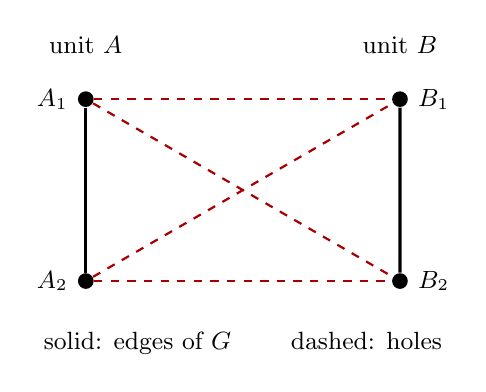
\begin{tikzpicture}[scale=1.05,every node/.style={font=\small}]
\node[circle,fill=black,inner sep=2pt,label=left:$A_1$] (a1) at (0,1.1) {};
\node[circle,fill=black,inner sep=2pt,label=left:$A_2$] (a2) at (0,-1.1) {};
\node[circle,fill=black,inner sep=2pt,label=right:$B_1$] (b1) at (3.8,1.1) {};
\node[circle,fill=black,inner sep=2pt,label=right:$B_2$] (b2) at (3.8,-1.1) {};
\draw[very thick] (a1)--(a2);
\draw[very thick] (b1)--(b2);
\draw[dashed,thick,red!65!black] (a1)--(b1);
\draw[dashed,thick,red!65!black] (a1)--(b2);
\draw[dashed,thick,red!65!black] (a2)--(b1);
\draw[dashed,thick,red!65!black] (a2)--(b2);
\node at (0,1.75) {unit \(A\)};
\node at (3.8,1.75) {unit \(B\)};
\node[align=center] at (1.9,-1.85)
{solid: edges of \(G\) \qquad dashed: holes};
\end{tikzpicture}
\caption{All four cross holes make the two solid matching edges
non-touching. The distribution theorem forces this conflict in every
unit law satisfying its marginal and joint density bounds.}
\label{fig:four-holes}
\end{figure}

To define holes, each sampled configuration carries injective linear
maps into common binary vector spaces. The coefficient spaces record
monomial evaluations \(v\) at Boolean points; their point moments
are the rank-one matrices \(vv\trans\). The frame maps induce an
embedding \(U_o\) of a space built from these moments, together with
a linear functional \(u_o\) on the ambient tensor space. Auxiliary
frame columns will be used to impose the cross-contraction equations.
A hole is certified by a shared tensor and two prescribed identities for the cross
contractions. The identities come from a symmetric bilinear form;
summing them around a hypothetical triangle cancels every bilinear
term and leaves \(0=1\). \Cref{sec:geometry} proves this parity
mechanism before constructing the particular moments and frames.

Forcing four holes is the harder task. The construction has one
unbounded parameter \(n\), and the ambient vector dimension is
\(N=M_0n\), with \(M_0\) fixed before the limit. The three main
steps are as follows.

\begin{enumerate}
\item
\emph{Finite certificates for four holes
(\Cref{sec:moments,sec:realization,sec:collision}).}
The candidate witnesses are short sums of point moments. A point's
\emph{key} is the tuple of its images under the relevant frame maps;
equal keys on the two sides give a shared tensor. We retain specified
images of a bounded number of coefficient directions, called
\emph{pins}. A fixed Boolean selector labels the points;
interpolation and a bounded set of excluded labels make the key
directions independent modulo these pins. A separate low-rank
moment decomposition identifies the obstructions to solving the
cross-contraction equations. Once the corresponding scalar conditions
hold, the remaining equations cost only \(O(n)\) bits. The collision
criterion in \Cref{prop:collision} reduces four holes to overlap of
the accepted key distributions. The witness sums use paired lists of
points, and a \emph{scalar recipe} prescribes their scalar conditions.
Sampling the point parameters with the configuration fixed will be
called a \emph{query}; its full key is the list of the point keys.

\item
\emph{Preparation of the unit law
(\Cref{sec:phases,sec:preparation}).}
Conditioning on exact pin images decomposes the law into parts called
\emph{leaves}, with control of every further independent image
prescription. A \emph{small table} records the cross pairings of the
projected pin directions and the auxiliary frame directions. The
scalar conditions must be compatible with this table. Phase estimates
produce compatible tables on a positive mass of independent unit
pairs, or on a smaller mass at least a fixed multiple of \(N^{-4}\)
determined by their leaves.

\item
\emph{Forcing overlap
(\Cref{sec:histograms,sec:product-tests,sec:common-limit,sec:status-span,sec:rare-overlap}).}
Each leaf's accepted key distributions have finite \(L^1\)
approximating families. Estimates for the mixed law also control
tests of single keys and the scalar values recorded with them.
A product comparison connects these single-position estimates to
tests of the full key tuple. If overlap vanished in the positive-mass
case, a common limit would rule out every scalar recipe whose matched
positions have positive overlap; finite-dimensional duality produces
precisely such a recipe. The inverse-polynomial compatibility mass
may disappear in this limit, so it is handled separately: a uniform large-set
estimate is applied to a finite family chosen on one leaf before
the independent opposite leaf is sampled.
\end{enumerate}

The Boolean moment argument uses commuting multiplication operators,
as in the flat-extension approach to moment problems
\citep{laurentmourrain2009}. The distribution-to-graph argument
combines information projection~\citep{csiszar1975}, independent-set
fingerprints~\citep{kleitmanwinston1982,samotij2015}, and a capacitated
cut~\citep{fordfulkerson1956}. The overlap estimates use entropy
\citep{cover2006} and the energy-increment method of weak regularity
\citep{frieze1999}; the additional constraints from the frame pairings
are retained explicitly in their proofs.

\subsection{Organization and conventions}

\Cref{sec:geometry,sec:distributions} define the frames and holes and
reduce the graph problem to uniform supersaturation.
\Cref{sec:frame-laws} establishes the frame-image estimates and the
decomposition into pinned leaves.
\Cref{sec:moments,sec:realization,sec:collision} prove the algebraic
realization and collision criteria.
\Cref{sec:phases,sec:preparation} prepare the unit law and its small
tables. The analytic comparison tools are established in
\Cref{sec:histograms,sec:product-tests}.
\Cref{sec:common-limit,sec:status-span} prove overlap on the branches
with positive limiting compatibility mass, and
\Cref{sec:rare-overlap} handles the remaining branch and completes the
proof. \Cref{sec:parameters} collects the order of choices and the
quantitative margins.

All vector spaces, matrices, ranks, and algebraic forms are over
\(\F\). Probabilities, densities, norms, and entropies are real.
Logarithms in bit counts have base two; changing the base for entropy
only changes fixed constants.
Constants described as bounded may be very large but are independent
of \(n\). An \(O(n)\) scalar record has its coefficient fixed before
\(M_0\) is chosen. Later fixed test accuracies and partition sizes may
change how large \(n\) must be; they do not change the construction.

The two endpoints in one unit may be dependent. Separate units, and
their leaves before additional pairing conditions, are sampled
independently. Query subdensities retain the mass lost to all
acceptance tests.

\section{The hole relation and its tensor realization}\label{sec:geometry}

The construction has two tasks. Its missing-edge relation must be
triangle-free, so that the resulting graph has independence number at
most two. It must also provide enough missing edges to prevent a large
connected matching. We first give the algebraic reason for
triangle-freeness. The tensor and frame construction that follows
provides the additional structure needed for the second task.

\subsection{A triangle-free relation}

Let \(\cX\) and \(\cV\) be finite-dimensional vector spaces over
\(\F\). Fix a linear functional \(a\in\cX^*\) and a symmetric
bilinear form \(T\) on \(\cX\), and write
\[
 r(x)=a+T(x,\cdot)\in\cX^*.
\]
Let \(\Omega\) be a finite set. For each \(i\in\Omega\), suppose
we have an injective linear map \(U_i:\cX\to\cV\) and a linear
functional \(u_i\in\cV^*\).

\begin{definition}\label{def:hole}
Two elements \(i,j\in\Omega\) have a \emph{hole} between them if
there exist \(\lambda_i,\lambda_j\in\cX\) such that
\begin{equation}\label{eq:hole-equations}
 \begin{gathered}
 U_i\lambda_i=U_j\lambda_j,\qquad
 u_jU_i=r(\lambda_i),\qquad u_iU_j=r(\lambda_j),\\
 a(\lambda_i)+a(\lambda_j)=1.
 \end{gathered}
\end{equation}
The middle two identities are identities of linear functionals on
the whole space \(\cX\).
\end{definition}

Thus a hole has a shared vector in \(\cV\), one witness for it in
each copy of \(\cX\), and opposite values of \(a\) on the witnesses.
The functional identities make these requirements incompatible around
a triangle.

\begin{lemma}\label{lem:hole-triangle-free}
The hole relation is symmetric, has no loops, and is triangle-free.
\end{lemma}
\begin{proof}
Symmetry follows by interchanging the endpoints.
A loop would have \(U_i\lambda_i=U_i\lambda_j\), hence
\(\lambda_i=\lambda_j\) by injectivity, contradicting the last
equation of \Cref{eq:hole-equations}.

Suppose that three distinct elements have holes on all three pairs.
For a directed incidence \(ij\), let \(x_{ij}\) be its witness at
\(i\). For distinct \(i,j,k\), evaluate the functional identity for
\(ij\) on \(x_{ik}\):
\[
 u_j(U_ix_{ik})=a(x_{ik})+T(x_{ij},x_{ik}).
\]
Sum over the six ordered choices of \((i,j,k)\).
For fixed \(j\), the two arguments on the left are equal by the
sharing equation for the remaining edge \(ik\), so they cancel.
For fixed \(i\), the two bilinear terms cancel by symmetry of \(T\).
The remaining sum is
\[
 \sum_{\{i,j\}}\bigl(a(x_{ij})+a(x_{ji})\bigr)=1+1+1=1,
\]
a contradiction.
\end{proof}

Given any list \(o_1,\ldots,o_m\in\Omega\), form a graph \(G\)
on its \emph{positions}: two distinct positions are adjacent when
their elements have no hole. This gives a finite simple graph even
when elements repeat. Equal elements are adjacent because holes have
no loops. An independent triple of positions would therefore give
three distinct elements forming a hole triangle. Hence
\begin{equation}\label{eq:sample-independence}
 \alpha(G)\le2,\qquad \chi(G)\ge\lceil m/2\rceil.
\end{equation}

It remains to choose the finite set and its linear data so that a
random list also has no large connected matching. Two disjoint edges
fail to touch precisely when all four cross pairs are holes. The
distribution theorem in \Cref{sec:distributions} will force these
four-hole conflicts for the model constructed below.

\subsection{Construction parameters}

We now construct \(\cX,a,T,\cV\) and the maps \(U_o,u_o\), together
with a uniform law \(\mu_n\) on a finite set \(\Omega_n\) of
frames. All vector spaces, maps, tensor products, and ranks remain over
\(\F\). We use the entrywise pairing of matrices:
\[
 \pair{A}{B}=\sum_{r,c}A_{rc}B_{rc}=\Tr(A\trans B).
\]
Probabilities and entropy take real values.

The sole asymptotic parameter is \(n\). All numerical construction
parameters are fixed independently of the law of units, in the order
specified in \Cref{sec:parameters}, before \(n\) tends to infinity.
Set
\begin{equation}\label{eq:early-constants}
 C_0=1000,\qquad g=10^9+1,\qquad
 D=4C_0g,\qquad M=2^{1000}.
\end{equation}
In particular, \(g\) is odd. The budgets for conditioning a unit law
are introduced in \Cref{sec:frame-laws}; they precede the selector
parameters \(j_*,b\) and the mixing parameters through \(J\) in
\Cref{sec:moments}. Choose \(r_0\) sufficiently large after those
choices, put \(h=1000r_0\), and choose the dimension multiplier
\(M_0\) last. The ambient dimension and sample size are
\begin{equation}\label{eq:parameter-order}
 N=M_0n,\qquad m=2^{C_0gN}.
\end{equation}
We take \(j_*\ge1\) and \(n\ge2r_0\). For each sufficiently
large \(n\), the matrices used below are chosen to satisfy
\Cref{lem:generic-mixers}, before any unit law is considered.

An \(O(n)\) bit count below has a coefficient fixed before \(M_0\)
and can therefore be made a prescribed small fraction of \(N\).
This is different from an \(o(N)\) bound: after \(M_0\) is fixed,
\(n/N=1/M_0\) is constant. Later fixed tests and tolerances may
increase the required lower bound on \(n\); they do not change the
construction.

\subsection{Moment matrices and cut profiles}

Let
\[
 \cI=\mathbb Z/g\mathbb Z,\qquad
 \cE=\binom{\cI}{2},\qquad
 I_d=\{d+1,\ldots,d+(g-1)/2\}\subset\cI .
\]
Elements of \(\cI\) are \emph{tags}; elements of \(\cE\) are \emph{components}.
The ordinary, or base, variables comprise \(g^2+3\) blocks of \(n\) bits:
\[
 O_{d,t}\quad(d,t\in\cI),\qquad S,\quad \#,\quad Z.
\]
A separate selector has \(b\) bits.  Its values \(s\in\F^b\) are called \emph{labels}, to distinguish them from tags.

The \(O\)-blocks carry testers whose availability depends on the tag,
while \(S\) carries a tester available at every tag.
The additional \(\#\)-block lets the self-Gram form \(E\), defined
below, distinguish different selector labels.
The \(Z\)-block is absent from \(E\); its free coordinates and
change-of-basis symmetry are used in the later parameter tests.

Let
\[
 p_*=\sum_{j=0}^{j_*}\binom bj,\qquad
 \cB=\F^{p_*}\otimes\F^{\,1+(g^2+3)n}.
\]
The first factor is indexed by squarefree selector monomials of degree at most \(j_*\); the second by the constant and the individual base variables.
If \(p_s\) is the vector of selector-monomial evaluations and \(z\) is a base value, write
\begin{equation}\label{eq:point-evaluation}
 v(s,z)=p_s\otimes(1,z)\in\cB.
\end{equation}
Thus the row and column coordinates both represent monomials of base degree at most one and selector degree at most \(j_*\).

Let \(W\subset\cB\otimes\cB\) be the span of the point moments \(v(s,z)v(s,z)\trans\).
For \(l\in\cI\), let \(W_l\) be the span of those point moments for which
\[
 O_{d,t}=0\quad\text{whenever }l\notin I_d.
\]
Let \(W_*\) be defined by requiring every \(O\)-block to be zero.
The cut-profile space is
\begin{equation}\label{eq:cut-profile-space}
 \cX=
 \left\{x=(x_{\{l,l'\}})_{\{l,l'\}\in\cE}:
 x_{\{l,l'\}}=w_l+w_{l'},\quad w_l\in W_l\right\}.
\end{equation}
A tuple \(w=(w_l)_{l\in\cI}\) as in this display is a \emph{representation} of \(x\).

\begin{lemma}\label{lem:cut-kernel}
The intersection of \(W_l\) over any strict majority of tags is \(W_*\).
Two representations of the same cut profile differ by a constant tuple with value in \(W_*\).
\end{lemma}
\begin{proof}
Fix a base coordinate in \(O_{d,t}\).  It is allowed at exactly \((g-1)/2\) tags.
A strict majority therefore contains a tag where that coordinate is disallowed.
Every row and column involving it is zero in \(W_l\) for that tag.
A matrix in the intersection consequently has zero rows and columns at all \(O\)-coordinates.

The coordinate projection that sets all \(O\)-variables to zero sends each point moment to a point moment defining \(W_*\).
Applied on both matrix factors, it fixes the matrix just described.
That matrix is therefore in \(W_*\), proving the nontrivial inclusion.

If \(w,w'\) give the same differences, then
\(w_l+w'_l=w_{l'}+w'_{l'}\) for every pair of tags.
Their difference is a constant tuple.  Its value belongs to every \(W_l\), hence to \(W_*\).
Conversely every such constant tuple lies in the kernel of the cut map.
\end{proof}

In each \(O_{d,t}\)-block and in \(S\), choose the first \(2r_0\) coordinates in disjoint ordered pairs.
The corresponding linear functionals on moments are
\[
 \eta_{d,t}\bigl(v(s,z)v(s,z)\trans\bigr)
   =\sum_{\rho=1}^{r_0}z_{O_{d,t},2\rho-1}z_{O_{d,t},2\rho},
 \qquad
 \eta_S\bigl(v(s,z)v(s,z)\trans\bigr)
   =\sum_{\rho=1}^{r_0}z_{S,2\rho-1}z_{S,2\rho}.
\]
They are well defined by selecting the indicated ordered matrix entries.
Put
\[
 \eta_O=\sum_{d,t}\eta_{d,t},\qquad \eta=\eta_O+\eta_S.
\]
For a cut profile represented by \(w\), define
\begin{equation}\label{eq:cut-functionals}
 \begin{aligned}
 a_t(x)&=\sum_{l,d}\eta_{d,t}(w_l),&
 a(x)&=\sum_t a_t(x)=\sum_l\eta_O(w_l),\\
 b_t(x)&=\sum_{l\ne t}\eta_S(w_l),&
 \chi_*(w)&=\sum_l\eta(w_l).
 \end{aligned}
\end{equation}
The functions \(a_t,a,b_t\) are well defined on \(\cX\).
Indeed, a constant kernel value in \(W_*\) contributes zero to every \(O\)-tester, while it contributes
\((g-1)\eta_S(w_*)=0\) to \(b_t\).
The quantity \(\chi_*(w)\) is used only when a representation has been specified.

Define a symmetric bilinear form \(T^0\) on \(\cX\) by
\begin{equation}\label{eq:T-zero}
 T^0=a\otimes a+\sum_{t\in\cI}(a_t\otimes b_t+b_t\otimes a_t).
\end{equation}
For \(1\le j\le J\) and ordered components \(e,f\), choose endomorphisms \(L_j^{ef},R_j^{ef}\) of \(\cB\).
Their required properties will be proved in \Cref{lem:generic-mixers}.
Set
\begin{equation}\label{eq:T-one}
 \begin{split}
 B^1(x,y)&=\sum_{j=1}^J\sum_{e,f\in\cE}
   \pair{x_e}{L_j^{ef}y_f(R_j^{ef})\trans},\\
 T^1(x,y)&=B^1(x,y)+B^1(y,x),\qquad T=T^0+T^1.
 \end{split}
\end{equation}
This specifies the symmetric form \(T\) in the hole equations and
hence the affine-gradient map \(r(x)=a+T(x,\cdot)\).
The integer \(r\) introduced in \Cref{eq:law-budgets} is a separate
rank budget.
Since the mixed terms in \(T^0(x,x)\) cancel, \(T^1\) is alternating, and \(a(x)^2=a(x)\), we have
\begin{equation}\label{eq:T-diagonal}
 T(x,x)=a(x)\qquad(x\in\cX).
\end{equation}

The prescribed self-frame Gram matrix is denoted by \(E\).
It is the sum of the ordered tester matrices for \(\eta\) and a matrix \(E^\#\) characterized on evaluation vectors by
\begin{equation}\label{eq:E-sharp}
 v(s,z)\trans E^\#v(s',z')
   =\sum_{\rho=1}^b(s_\rho+s'_\rho)\,z_\#\trans M_\rho z'_\# ,
\end{equation}
where \(M_\rho\) are \(n\)-by-\(n\) matrices chosen in \Cref{lem:generic-mixers}.
The expression is a bilinear form on \(\cB\) because \(j_*\ge1\).
It vanishes when the two point inputs coincide.
Consequently
\begin{equation}\label{eq:E-moments}
 \pair{E}{w}=\eta(w)\qquad(w\in W).
\end{equation}
The \(Z\)-block does not occur in \(E\).
In particular, any invertible linear change of the \(Z\)-variables preserves \(E\); this symmetry will be used in unary probability estimates.

\subsection{Raw vertices}

For each \(e\in\cE\), take copies \(V_e^+,V_e^-\) of \(\F^N\), paired by the usual dot product.
We regard \(V_e^-\) as the dual of \(V_e^+\) through that pairing.
A raw vertex, also called an \emph{orientation}, consists at each component of four maps
\[
 P_e,Q_e:\cB\longrightarrow V_e^+,V_e^-,
 \qquad X_e,Y_e:\F^h\longrightarrow V_e^+,V_e^-,
\]
where the target is the first or second one as appropriate.
They satisfy
\begin{equation}\label{eq:raw-frame-law}
 [P_e,X_e]\text{ and }[Q_e,Y_e]\text{ are injective},\qquad
 P_e\trans Q_e=E,\quad X_e\trans Q_e=0,\quad P_e\trans Y_e=0.
\end{equation}
No value is prescribed for \(X_e\trans Y_e\).

Write \(d=\dim\cB\).
For all large \(n\), \(N\ge2(d+h)\), by the final choice of \(M_0\).
The frame set is then nonempty.
For example, take the plus columns to be the first \(d+h\) coordinate vectors.
Prescribe the full \((d+h)\)-square Gram matrix to be
\(\begin{psmallmatrix}E&0\\0&0\end{psmallmatrix}\).
Lift its columns to minus vectors using the first \(d+h\) coordinates, and append distinct coordinate vectors in a complementary space of dimension \(d+h\).
These minus columns are independent and have the desired Gram values.

Take the uniform distribution on this finite frame set, independently over components.
Let \(\Omega_n\) be the raw vertex space and \(\mu=\mu_n\) this distribution.
There are at most \(2^{2|\cE|N(d+h)}\) raw vertices, so
\begin{equation}\label{eq:raw-space-size}
 \log_2|\Omega_n|=O(N^2).
\end{equation}

Use the common ambient tensor space
\[
 \cV=\bigoplus_{e\in\cE}V_e^+\otimes V_e^-.
\]
For a raw vertex \(o\), define
\begin{equation}\label{eq:raw-embedding}
 U_o x=(P_{o,e}x_eQ_{o,e}\trans)_{e\in\cE},
 \qquad
 u_o(\xi)=\sum_{e\in\cE}\pair{Y_{o,e}X_{o,e}\trans}{\xi_e}.
\end{equation}
On a simple tensor \(pq\trans\) in component \(e\), the latter pairing is
\[
 u_o(pq\trans)=(Y_{o,e}\trans p)\cdot(X_{o,e}\trans q).
\]
Thus the minus channel is paired with the first tensor factor and the plus channel with the second.
All copies of coefficient spaces attached to different vertices are distinct, although the ambient \(V_e^\pm\) are common.

Each \(U_o\) is injective: a left inverse of \(P_{o,e}\) and the transpose of a left inverse of \(Q_{o,e}\) recover \(x_e\) from \(P_{o,e}x_eQ_{o,e}\trans\).
The two annihilator conditions in \Cref{eq:raw-frame-law} also give
\begin{equation}\label{eq:self-contraction-zero}
 u_oU_o=0.
\end{equation}

We have now supplied all the linear data of \Cref{def:hole}.
By \Cref{lem:hole-triangle-free}, their hole relation on
\(\Omega_n\) is symmetric, loopless, and triangle-free.
Sample \(m\) raw vertices independently with law \(\mu_n\), and
form the graph on their positions as above. Equation
\eqref{eq:sample-independence} gives \(\alpha(G)\le2\)
deterministically. The next section reduces the bound on its
connected matchings to a distribution statement for this frame law.

\section{From supersaturation to a finite graph}\label{sec:distributions}

A \emph{unit} is an ordered pair of raw vertices with no hole between its endpoints.
The endpoints of a unit may be dependent.
When two units are sampled independently, their four endpoints need not be independent within either unit.
The event of interest is that all four cross pairs have holes, as in \Cref{fig:four-holes}.

\begin{theorem}[Raw supersaturation]\label{thm:raw-supersaturation}
For the construction parameters specified in \Cref{sec:geometry,sec:parameters}, for all sufficiently large \(n\), every probability law \(\sigma\) on units satisfying
\begin{equation}\label{eq:raw-law-caps}
 \sigma_1\le M\mu,\qquad \sigma_2\le M\mu,\qquad
 \sigma\le 2^{DN}\mu^2
\end{equation}
has the following property: two independent units drawn from \(\sigma\) have all four cross holes with probability at least \(2^{-100gN}\).
The inequalities in \Cref{eq:raw-law-caps} are pointwise inequalities of measures on the finite raw spaces.
\end{theorem}

The proof of \Cref{thm:raw-supersaturation} occupies the subsequent sections and is completed in \Cref{sec:rare-overlap}.
We prove its implication for graphs here. The frame estimates and the preparation of an admissible unit law begin in \Cref{sec:frame-laws}.

\subsection{Entropy minimizers and terminal cuts}

We use a finite form of the information-projection argument of
Csisz\'ar~\citep{csiszar1975}. Its support assertion is important here:
the minimizing law must see every point that can occur in a feasible law.
Relative entropy is taken with natural logarithms:
\[
 \mathsf D(\rho\Vert q)=\sum_x\rho(x)\log\frac{\rho(x)}{q(x)}.
\]
Here \(q\) is a strictly positive probability measure and \(0\log0=0\).

\begin{lemma}\label{lem:entropy-support}
Let \(\mathcal P\) be a nonempty compact convex set of probability measures on a finite set, and let \(\rho\) minimize \(\mathsf D(\cdot\Vert q)\) on \(\mathcal P\).
Then \(\rho\) is positive on the union of the supports of measures in \(\mathcal P\).
For every \(\rho'\in\mathcal P\),
\[
 \mathsf D(\rho'\Vert q)-\mathsf D(\rho\Vert q)
 \ge \mathsf D(\rho'\Vert\rho).
\]
If \(\rho'\) is supported on a set \(S\), the right side is at least \(-\log\rho(S)\).
\end{lemma}
\begin{proof}
If \(\rho(x)=0<\rho'(x)\) at a feasible support point, the entropy along
\((1-t)\rho+t\rho'\) has right derivative \(-\infty\) at zero from the newly occupied points.
At all points where \(\rho>0\), its derivative is finite.
This contradicts minimality, proving the support assertion.

We can therefore differentiate toward any feasible \(\rho'\) using only points where \(\rho>0\).
The right derivative at the minimizer is nonnegative, giving
\[
 \sum_x(\rho'(x)-\rho(x))\log\frac{\rho(x)}{q(x)}\ge0,
\]
where the constant derivative term cancels because both measures have total mass one.
The exact identity
\[
 \mathsf D(\rho'\Vert q)-\mathsf D(\rho\Vert q)
 =\mathsf D(\rho'\Vert\rho)
  +\sum_x(\rho'(x)-\rho(x))\log\frac{\rho(x)}{q(x)}
\]
proves the second assertion.
Finally, if \(\rho'\) is supported on \(S\), comparison with the normalized restriction \(\rho(\cdot\mid S)\) gives
\[
 \mathsf D(\rho'\Vert\rho)
 =\mathsf D(\rho'\Vert\rho(\cdot\mid S))-\log\rho(S)
 \ge-\log\rho(S).
\]
For completeness, nonnegativity of relative entropy follows from
\(\log t\le t-1\), applied with \(t=q(x)/\rho'(x)\) and summed over the positive support of \(\rho'\).
\end{proof}

The next lemma is the max-flow/min-cut principle of
Ford and Fulkerson~\citep{fordfulkerson1956} with capacities chosen
to encode the three density bounds. We include the finite residual-cut
argument, which applies to the real capacities used here.

\begin{lemma}\label{lem:terminal-cut}
Let \(R\subseteq\Omega_n^2\).
If no probability law supported on \(R\) satisfies \Cref{eq:raw-law-caps}, there are sets \(S\subseteq\Omega_n\) and \(E_0\subseteq\Omega_n^2\) such that
\[
 \mu(S)<1/M,\qquad \mu^2(E_0)<2^{-DN},
\]
and every pair in \(R\) either has an endpoint in \(S\) or belongs to \(E_0\).
\end{lemma}
\begin{proof}
Construct a directed network with source \(s\), a left copy and a right copy of \(\Omega_n\), and sink \(t\).
Give the edge from \(s\) to left \(x\) capacity \(M\mu(x)\), the edge from right \(y\) to \(t\) capacity \(M\mu(y)\), and the edge from left \(x\) to right \(y\) capacity
\(2^{DN}\mu(x)\mu(y)\) whenever \((x,y)\in R\).
A flow of value one is precisely a law satisfying the three caps.
A flow of larger value could be scaled down to value one, so the maximum value is less than one.

The feasible flows form a compact polytope, hence the flow value has a maximizer \(f\).
In its residual network, include a forward edge whenever its capacity exceeds its flow and a reverse edge whenever its flow is positive.
There is no residual path from \(s\) to \(t\): augmenting by the smallest positive residual capacity on such a path would increase the value.
Let \(Z\) be the vertices reachable from \(s\).
Every forward edge across \(Z\) to its complement is saturated, and every forward edge in the opposite direction has zero flow, since otherwise its reverse residual edge would leave \(Z\).
Summing flow conservation over \(Z\) shows that the capacity of this cut equals the value of \(f\), hence is less than one.

Let \(L_0\) be the raw types whose left copies are outside \(Z\), and let \(R_0\) be those whose right copies are in \(Z\).
The cut-capacity inequality is
\[
 M\mu(L_0)+M\mu(R_0)
 +2^{DN}\mu^2\bigl(R\cap((\Omega_n\setminus L_0)
                         \times(\Omega_n\setminus R_0))\bigr)<1.
\]
Take \(S=L_0\cup R_0\) and take \(E_0\) to be the pair set in the last summand.
Its measure and that of \(S\) have the asserted bounds.
A pair in \(R\) with neither endpoint in \(S\) necessarily belongs to \(E_0\).
\end{proof}

\subsection{Containers and the random sample}

We now adapt the independent-set fingerprint method of
Kleitman and Winston~\citep{kleitmanwinston1982}; see also
\citet[Section~2]{samotij2015}. Here the progress measure is the minimum
relative entropy of a feasible law. The preceding cut lemma handles
the terminal set when no such law remains.

\begin{proposition}\label{prop:raw-to-graph}
Assume the conclusion of \Cref{thm:raw-supersaturation} at a given sufficiently large \(n\).
For \(m=2^{C_0gN}\), the sampled graph defined in \Cref{sec:geometry} satisfies
\[
 \alpha(G)\le2,\qquad \cm(G)<m/100
\]
with probability \(1-\exp(-\Omega(m))\).
The implied positive constant is independent of \(n\).
\end{proposition}
\begin{proof}
\textbf{Entropy-controlled fingerprints.}
Make a finite \emph{conflict graph} whose vertices are raw units; two units are adjacent when they give all four cross holes.
There are no loops, since a repeated unit would require a hole from a raw vertex to itself.
Put \(\varepsilon_N=2^{-100gN}\).

For an independent set \(I\) of raw units, start with all units as a residual set \(R\).
If there is a feasible law satisfying \Cref{eq:raw-law-caps} on \(R\), choose its relative-entropy minimizer with respect to \(\mu^2\).
Such a minimizer exists because the feasible laws form a compact convex polytope and relative entropy is continuous on the finite probability simplex.
Fix deterministic choices throughout.
The average, under this law \(\rho\), of \(\rho(N_R(v))\) is the conflict probability of two independent \(\rho\)-units, so is at least \(\varepsilon_N\).
Choose a unit \(v\in R\) maximizing this neighborhood mass.
If \(v\in I\), record \(v\) and delete its entire neighborhood \(N_R(v)\).
If \(v\notin I\), delete \(v\) alone.
Both operations preserve \(I\subseteq R\).
Each removes at least one unit, so the procedure terminates at a residual set with no feasible law.

When a recording leaves a feasible residual, \Cref{lem:entropy-support} shows that the new minimum entropy exceeds the old one by at least
\(-\log(1-\varepsilon_N)\).
Other deletions cannot decrease the minimum.
Every feasible law has entropy in \([0,DN\log2]\), since its density is at most \(2^{DN}\).
Allowing one final recording that leaves no feasible residual, the fingerprint has length at most
\begin{equation}\label{eq:fingerprint-length}
 L_N=1+\left\lceil
       \frac{DN\log2}{-\log(1-\varepsilon_N)}
      \right\rceil
 =O(1+DN\,2^{100gN}).
\end{equation}

The fingerprint determines the terminal set.
Indeed, after a unit is recorded its residual neighborhood is empty, and remains empty as residual sets shrink.
A feasible law always has a unit with strictly positive neighborhood mass, so a recorded unit is never selected again.
Given the set of recorded units, replay the deterministic procedure, recording a selected unit exactly when it is in that set.
All other selected units are deleted.
This reproduces every step and the terminal set.

By \Cref{eq:raw-space-size}, the logarithm of the number of raw units is \(O(N^2)\).
The number of possible fingerprints, and hence terminal sets, is at most
\((|\Omega_n|^2+1)^{L_N}\).
Its logarithm is
\begin{equation}\label{eq:container-count}
 O(N^3\,2^{100gN})=o(m),
\end{equation}
since \(m=2^{1000gN}\).

\medskip\noindent\textbf{Terminal exceptions in the sample.}
For each terminal set fix sets \(S,E_0\) supplied by \Cref{lem:terminal-cut}.
Let \(k=\lceil m/200\rceil\).
The probability that at least \(k\) sampled positions have raw type in \(S\) is at most
\[
 \binom mk\mu(S)^k
 \le \left(\frac{em}{kM}\right)^k
 \le (200e/M)^k
 =\exp(-\Omega(m)).
\]
A fixed collection of \(k\) disjoint ordered pairs of distinct sampled positions consists of independent \(\mu^2\)-draws.
It lies entirely in \(E_0\) with probability at most \(2^{-kDN}\).
There are at most \(m^{2k}\) such collections, so the probability that one exists is at most
\begin{equation}\label{eq:pair-exception-bound}
 m^{2k}2^{-kDN}
 =2^{(2C_0g-D)Nk}
 =2^{-2C_0gNk}.
\end{equation}
Union over the \(\exp(o(m))\) terminal sets using \Cref{eq:container-count}.
Outside a set of probability \(\exp(-\Omega(m))\), every terminal set has fewer than \(m/200\) exceptional positions and fewer than \(m/200\) disjoint position pairs in its pair exception.
The strict bounds follow from \(k-1<m/200\).

Suppose on this event that \(G\) has a touching matching of size at least \(m/100\).
Orient its edges arbitrarily, and let \(I\) be the set of raw unit types thereby realized.
This is independent in the conflict graph: four cross holes would mean that the two endpoint sets have no edge between them in \(G\).
Different sampled matching edges may have the same raw type; no injectivity of this assignment is needed.
Run the container procedure for this set \(I\).
Every occurrence of a matching-edge type lies in its terminal set, and hence is covered by \(S\) or \(E_0\).
Because the matching uses disjoint sampled positions, fewer than \(m/200\) of its edges can meet the positions in \(S\).
The rest give disjoint ordered position pairs in \(E_0\), of which there are also fewer than \(m/200\).
Their sum is less than \(m/100\), a contradiction.

Finally, \(\alpha(G)\le2\) holds deterministically by \Cref{lem:hole-triangle-free}.
\end{proof}

\subsection{The clique-minor bound}

\Cref{prop:raw-to-graph} supplies the required bound on connected
matchings once raw supersaturation is proved. The next counting
argument converts that bound into the clique-minor estimate used in
the introduction.

The following elementary estimate counts small branch sets, in the
same connected-matching approach used by Cambie~\citep{cambie2021}.
Its deliberately coarse bound holds for every finite graph.

\begin{proposition}\label{prop:matching-minor}
For every finite nonempty graph \(G\) of order \(m\),
\[
 \had(G)\le\frac{m+4\cm(G)+2}{3}.
\]
In particular, if \(\alpha(G)\le2\) and \(\cm(G)<m/100\), then
\[
 \had(G)<\frac{26m}{75}+\frac23<\frac m2\le\chi(G)
 \qquad(m\ge5).
\]
\end{proposition}
\begin{proof}
Consider a complete-minor model with \(b\) branch sets.
Let \(s\) of them be singletons and \(e\) have two vertices.
Each two-vertex branch is an edge.
The singleton vertices form a clique, so pairing them gives \(\lfloor s/2\rfloor\) more edges.
All these edges together form one touching matching: their vertex sets are disjoint, and adjacency of the original branches guarantees every required contact.
Writing \(c=\cm(G)\), we obtain
\[
 c\ge e+\lfloor s/2\rfloor,\qquad s\le2(c-e)+1.
\]
Every remaining branch has at least three vertices, whence
\[
 m\ge s+2e+3(b-s-e)=3b-2s-e.
\]
Combining the inequalities gives
\[
 3b\le m+2s+e\le m+4c-3e+2\le m+4c+2.
\]
Maximize over all complete-minor models.
For the final assertion, every color class has at most two vertices when \(\alpha(G)\le2\), so \(\chi(G)\ge m/2\).
Combine this with \(c<m/100\) and \(26m/75+2/3<m/2\) when \(m\ge5\).
\end{proof}

\section{Frame laws and preparation of unit laws}\label{sec:frame-laws}

We now prepare the probability laws used to prove raw supersaturation.
Under the reference law \(\mu^2\), prescribed vector images have
exponentially small probabilities, even when their nominal directions
combine both endpoints of a unit. This will imply two useful properties
of any law satisfying \Cref{eq:raw-law-caps}. After discarding
exponentially small mass, tensors shared by its endpoints have sparse
profiles, and the law can be partitioned into
parts on which every unpinned exact-image constraint remains unlikely.
The normalized laws of these parts will be called leaf laws.

\subsection{Uniform frame laws}

We record the linear algebra behind all reference image laws.
For a subspace of a nominal coefficient space, its \emph{image} is its image under the relevant frame map.
Nominal independence is independence before applying these maps.

\begin{lemma}\label{lem:paired-frame-orbit}
Let \(A,A':U\to V\) and \(B,B':W\to V^*\) be injective maps between finite-dimensional spaces over \(\F\).
If
\[
 B\trans A=(B')\trans A',
\]
there is \(L\in\GL(V)\) with \(LA=A'\) and \(L^{-\mathsf T}B=B'\).
Thus based individually injective plus and minus frames with a prescribed Gram matrix form one orbit under the simultaneous primal and dual action.
\end{lemma}
\begin{proof}
Write \(\Phi=B\trans:V\to W^*\) and \(\Phi'=(B')\trans:V\to W^*\).
Both are surjective.
The based map \(f:A(U)\to A'(U)\) given by \(f(Au)=A'u\) satisfies \(\Phi'f=\Phi\).
It therefore maps \(A(U)\cap\ker\Phi\) isomorphically onto \(A'(U)\cap\ker\Phi'\).
Extend this restriction to an isomorphism \(L_0:\ker\Phi\to\ker\Phi'\).

Choose a complement \(U_0\) of \(A(U)\cap\ker\Phi\) in \(A(U)\).
Its images under \(\Phi\) are independent.
Extend a basis of \(\Phi(U_0)\) to a basis of \(W^*\), and choose lifts of the added basis vectors under \(\Phi\) and \(\Phi'\), respectively.
For the basis vectors in \(\Phi(U_0)\), choose the lifts in \(U_0\) and their images under \(f\).
Define \(L\) to equal \(L_0\) on \(\ker\Phi\) and to carry each chosen lift to its primed lift.
These are direct-sum decompositions of \(V\), so \(L\) is an isomorphism.
It extends \(f\) and satisfies \(\Phi'L=\Phi\), which is equivalent to the two required frame identities.
\end{proof}

\begin{lemma}[Gram normalization]\label{lem:gram-frame-normalization}
Let \(p,q\) be nonnegative integers with \(p+q\le N\).
For \(p\) independent uniform plus vectors and \(q\) independent uniform minus vectors in paired copies of \(\F^N\), and a prescribed \(p\)-by-\(q\) Gram matrix \(G\), the probability of that Gram matrix together with individual injectivity of both frames is at most \(2^{-pq}\) and at least
\begin{equation}\label{eq:bounded-gram-normalization}
 2^{-pq}(1-2^{p-N})(1-2^{p+q-N}).
\end{equation}
In particular, any consistent Gram specification on a bounded number of vectors, together with injectivity on each side, has probability bounded below by a positive constant for large \(N\).
\end{lemma}
\begin{proof}
The plus columns are linearly independent with probability at least \(1-2^{p-N}\): each nonzero coefficient dependence has probability \(2^{-N}\).
Given their linear independence, each minus column takes its required evaluations with probability \(2^{-p}\), independently, so the Gram costs \(2^{-pq}\).
Under this Gram conditioning, every nonzero combination of minus columns is uniform on an affine space of dimension at least \(N-p\).
Its probability of vanishing is at most \(2^{-(N-p)}\).
Union over fewer than \(2^q\) combinations gives failure probability at most \(2^{p+q-N}\).
This proves the lower bound.
For the upper bound with plus injectivity required, condition on the plus columns and use the exact \(2^{-pq}\) Gram probability whenever they are independent.
A partially specified consistent Gram contains some full specification; for bounded \(p,q\), the same positive lower bound for that full specification proves the last assertion.
\end{proof}

\begin{lemma}\label{lem:frame-images}
The following statements hold for all sufficiently large \(n\).
\begin{enumerate}[label=\textup{(\alph*)}]
\item
The plus frame \([P,X]\) is uniform among injective maps.
Conditional on it, the minus columns are independent uniforms on the affine spaces prescribed in \Cref{eq:raw-frame-law}, followed only by the conditioning that \([Q,Y]\) is injective.
The failure probability of this last condition, before conditioning, is at most \(2^{2(d+h)-N}\) per component.

Given \(P,Q\), the channels \(X,Y\) are independent uniform-column draws on \(\ker Q\trans\) and \(\ker P\trans\), respectively, conditioned on \([P,X]\) and \([Q,Y]\) being injective.
The two rank-failure probabilities are exponentially small in \(N\).
Each channel frame alone is uniform among injective maps \(\F^h\to\F^N\).
For any fixed \(q\) independent vectors in its paired ambient space, the probability that transpose evaluation on their span is not injective is at most
\begin{equation}\label{eq:channel-transpose-failure}
 2^{q-h+1}.
\end{equation}
The unconditional joint channel law is bounded above by a constant, depending on \(g,h\) but not on \(n\), times the completely independent uniform-column law.

\item
At independently sampled raw vertices and components, images of prescribed primal coefficient tuples that are independent separately at each vertex and sign are uniform subject to their individual injectivities and their prescribed same-vertex Gram matrices.
For tuples using channels as well, the same assertion holds conditionally on the full self-channel Gram matrices \(X_e\trans Y_e\); the relevant full Gram matrix is
\(\begin{psmallmatrix}E&0\\0&X_e\trans Y_e\end{psmallmatrix}\).

\item
Let a fixed tuple of nominal directions use arbitrary combinations of the two endpoints' primal and channel coefficients.
Compute its rank separately in each component and sign in the \emph{direct sum over both endpoints}, and let the total be \(t\).
For every preassigned \(\epsilon>0\), choosing \(M_0\) sufficiently large gives, under \(\mu^2\),
\begin{equation}\label{eq:reference-image-cap}
 \PP\{\text{all those images equal prescribed vectors}\}
 \le 2^{-(1-\epsilon)tN}\qquad(t\ge1).
\end{equation}
This is valid for all possible ranks \(t\), including \(t=O(n)\), not only for bounded tuples.
\end{enumerate}
\end{lemma}
\begin{proof}
The raw law is invariant under \(L\) on each \(V_e^+\) and \(L^{-\mathsf T}\) on \(V_e^-\), independently at vertices and components.
For (a), the action is transitive on injective plus frames, so their marginal is uniform.
Given a plus frame, each column of \(Q\) has specified evaluations against \(P,X\), while each column of \(Y\) has zero evaluations against \(P\).
There is no other constraint until full minus injectivity is imposed.
The remaining allowed set is therefore the product of those affine column spaces restricted to full rank.

Each column space contains the common translation space
\(\operatorname{ann}(\im[P,X])\), of dimension \(N-d-h\).
For a nonzero coefficient vector \(c\in\F^{d+h}\), the corresponding linear combination of minus columns is consequently uniform on an affine space containing that translation space.
Its chance of being zero is at most \(2^{-(N-d-h)}\).
Union over the fewer than \(2^{d+h}\) nonzero coefficient vectors gives the asserted bound \(2^{2(d+h)-N}\).

Alternatively, condition first on \(P,Q\).
The allowed \(X\)-columns lie in \(\ker Q\trans\), the allowed \(Y\)-columns in \(\ker P\trans\), and their two full-rank restrictions are separate.
This proves the stated conditional independence.
For example, before imposing injectivity of \([P,X]\), any dependence with a nonzero \(X\)-coefficient has probability at most \(2^{-(N-d)}\); union over its at most \(2^{d+h}\) coefficient choices gives a bound \(2^{2d+h-N}\).
The estimate for \(Y\) is identical.

The marginal of \(X\) alone is invariant under \(\GL(\F^N)\) and supported on injective maps; transitivity gives its uniformity, and likewise for \(Y\).
Before conditioning independent channel columns to be injective, their evaluations on a fixed independent \(q\)-tuple form a uniform \(h\)-by-\(q\) matrix.
For each nonzero coefficient vector in \(\F^q\), the chance that its evaluation is zero is \(2^{-h}\).
Union over those coefficient vectors gives at most \(2^{q-h}\), and channel injectivity has probability at least \(1/2\) for large \(N\).
This proves \Cref{eq:channel-transpose-failure}.
To compare their joint marginal with completely independent columns, condition on \(G=X\trans Y\).
The conditional marginal is uniform on the orbit of two individually injective \(h\)-frames having Gram matrix \(G\).
Under independent uniform columns that orbit has probability at least \(2^{-h^2-2}\) for large \(N\), by \Cref{lem:gram-frame-normalization}.
Since the raw probability of any \(G\) is at most one, the density ratio on every such orbit is at most \(2^{h^2+2}\).
Multiply over the fixed number of components to obtain the joint channel bound.
Its possible dependence on \(h\) is harmless: \(h\) is fixed before \(n\) grows.

For (b), the restricted Gram of primal tuples is fixed by \(E\).
By \Cref{lem:paired-frame-orbit}, all based realizations with that Gram and individual injectivity lie in one orbit.
Projection of an invariant uniform raw law is uniform on this orbit: an element carrying one partial realization to another bijects their full-frame completions.
There is at least one completion because these tuples are restrictions of a raw frame.
After fixing \(X_e\trans Y_e\), the same argument applies to arbitrary full-frame coefficient tuples.
Independence over raw draws and components proves (b).

For (c), we prove the image cap, keeping explicit the dependence on the rank.
Replace each tested tuple by a basis of its nominal span; inconsistent dependent prescriptions have probability zero.
For the plus directions at the two endpoints, start with completely independent uniform plus columns and then impose individual full-frame injectivity.
The image of a rank-\(t_+\) tuple in the joint nominal direct sum is exactly uniform on \(t_+\) independent ambient vectors before this conditioning.
Indeed, at each ambient coordinate the coefficient map is a surjective linear map onto \(\F^{t_+}\), and different ambient coordinates use independent input bits.
Full injectivity has probability \(1-2^{-\Omega(N)}\), uniformly over the given construction, so the plus prescription costs at most
\((1-2^{-\Omega(N)})^{-1}2^{-t_+N}\).

Now condition on all plus frames.
At a component let \(S\) be the span of both endpoints' plus columns; then \(\dim S\le2(d+h)\).
Before minus injectivity, every minus column has an affine distribution whose translation space contains \(S^\perp\).
Split off an independent uniform \(S^\perp\)-part of each column and condition on the remaining parts.
For a rank-\(t_-\) tuple of minus coefficient combinations, the \(S^\perp\)-parts of its images are independent uniform vectors in \(S^\perp\), because the coefficient map has rank \(t_-\).
Thus prescribed minus images have probability at most
\[
 2^{-(N-2(d+h))t_-}.
\]
The additional conditioning on the two minus frames being injective changes this by a factor \(1+2^{-\Omega(N)}\), by (a).
Perform this argument componentwise.
There is a fixed total conditioning factor bounded, for example, by \(4^{|\cE|}\), and the resulting bound is
\[
 4^{|\cE|}\,2^{-t_+N-(N-2(d+h))t_-}.
\]
Choose \(M_0\) so that \(2(d+h)/N<\epsilon/2\) for large \(n\), and then increase \(n\) so that the fixed prefactor is at most \(2^{\epsilon N/2}\).
Since \(t=t_++t_-\ge1\), this proves \Cref{eq:reference-image-cap} uniformly for every allowable \(t\).
In particular, mixing the two endpoints in a direction causes no loss of an entire \(N\)-bit image constraint.
\end{proof}

\subsection{Sparse profiles arising from true intersections}

For a matrix profile, its \emph{total component rank} means \(\sum_{e\in\cE}\rank x_e\).

\begin{lemma}\label{lem:raw-intersections}
Let \(\sigma\) satisfy the joint cap in \Cref{eq:raw-law-caps}.
Outside a set of \(\sigma\)-probability \(2^{-\Omega(N)}\),
\[
 \sum_{e\in\cE}
  \dim\bigl(\im P_{1,e}\cap\im P_{2,e}\bigr)\le2D.
\]
For any unit outside that exceptional set and any
\(U_1\lambda_1=U_2\lambda_2\), both \(\lambda_i\) have total component rank at most \(2D\).
Each has a unique representation \((w_{i,l})_l\) vanishing at a strict majority of tags, and
\[
 |\{l:w_{i,l}\ne0\}|\le4D/g,\qquad
 \chi_*(w_1)=\chi_*(w_2).
\]
\end{lemma}
\begin{proof}
If the summed intersection dimension exceeds \(2D\), choose \(2D\) independent common-image vectors, componentwise.
Write each as \(P_{1,e}a=P_{2,e}b\).
Their nominal relation directions \((a,b)\) are independent in the direct sum of the two primal coefficient spaces at that component.
Indeed a dependence between the pairs would, after applying \(P_{1,e}\), be the corresponding dependence between the selected common-image vectors.
Across components their ranks add.

There are at most \(2^{O(n)}\) ways to choose this bounded number of coefficient pairs and their component indices.
For each choice, \Cref{eq:reference-image-cap} bounds the probability of their zero images by \(2^{-(1-\epsilon)2DN}\) under \(\mu^2\).
After paying \(2^{DN}\) for \(\sigma\), and making the coefficient count a sufficiently small fraction of \(N\) by the choice of \(M_0\), the union bound is \(2^{-\Omega(N)}\).

Suppose \(U_1\lambda_1=U_2\lambda_2=\xi\).
The column space of \(\xi_e\) lies in both primal plus spans.
Since multiplication by the two injective frame maps preserves matrix rank,
\[
 \rank(\lambda_{i,e})=\rank(\xi_e)
 \le\dim(\im P_{1,e}\cap\im P_{2,e}).
\]
This proves the total-rank assertion.

Take any representation \((w_l)_l\) of one of the profiles.
A component \(w_l+w_{l'}\) is nonzero whenever \(w_l\ne w_{l'}\), so there are at most \(2D\) unequal unordered pairs.
If no value occurred at a strict majority of tags, write \(c_v\) for its multiplicities.
Then
\[
 \#\{\text{unequal pairs}\}
 =\frac12\left(g^2-\sum_vc_v^2\right)
 \ge\frac12\left(g^2-\frac g2\sum_vc_v\right)
 =\frac{g^2}{4}>2D,
\]
a contradiction.
Let the majority have size \(g-z\).
There are at least \(z(g-z)\ge zg/2\) unequal pairs, hence \(z\le4D/g\).
Its common value belongs to \(W_*\) by \Cref{lem:cut-kernel}, so subtract it from every coordinate.
The resulting representation vanishes at a strict majority.
It is unique: two such representations differ by a constant, and their two majority zero sets intersect.

Finally, equality of the component tensors gives equality of their ambient traces.
By cyclicity of trace and \Cref{eq:E-moments},
\[
 \Tr(P_{i,e}\lambda_{i,e}Q_{i,e}\trans)
 =\pair{P_{i,e}\trans Q_{i,e}}{\lambda_{i,e}}
 =\eta(\lambda_{i,e}).
\]
For \(e=\{l,l'\}\), it follows that
\[
 \eta(w_{1,l})+\eta(w_{2,l})
 =\eta(w_{1,l'})+\eta(w_{2,l'}).
\]
This value is independent of the tag.
The two sparse representations together have at most \(8D/g=32000<g\) nonzero coordinates, so some tag has both entries zero.
The common value is therefore zero.
Summing over tags proves equality of the two specified \(\chi_*\)-values.
\end{proof}

\subsection{Peeling into leaves with exact pins}

We partition almost all of a capped unit law into leaves by storing
unusually likely exact-image constraints in bounded-dimensional pin spaces.
The remaining directions then satisfy a uniform image-probability bound.
For a unit \(O=(1,2)\), introduce nominal coefficient spaces at each component
\[
 \cL_{O,e}
   =\bigoplus_{i\in O}(\cB_i\oplus H_i^+),
 \qquad
 \cR_{O,e}
   =\bigoplus_{i\in O}(\cB_i\oplus H_i^-),
 \qquad H_i^\pm=\F^h.
\]
Their frame-image maps add the endpoint images in the common ambient \(V_e^\pm\).
A \emph{pin space} is a specified subspace \(D_{O,e}^\pm\) of this nominal direct sum together with specified exact images of every vector in a chosen basis.
It may mix both endpoints, and it may mix primal and channel coordinates.
Once the basis images are known, every image on the pin space is fixed.

For a tested tuple of directions, its \emph{rank modulo the pins} is the sum, over components and signs, of the dimensions of the spans of its classes in the nominal quotients by \(D_{O,e}^\pm\).
The rank is nominal; it is not computed after applying the raw frames.

The budgets for this procedure are fixed before the selector, mixer,
and channel parameters in the construction. Their values are
\begin{equation}\label{eq:pin-budgets}
 \begin{gathered}
 k_{\max}=56(g-1),\qquad
 \zeta=\frac{1}{1000k_{\max}},\qquad
 K_1=\left\lceil\frac{4(D+1)}{\zeta}\right\rceil.
 \end{gathered}
\end{equation}
The phase and second-pinning budgets are
\begin{equation}\label{eq:law-budgets}
 \begin{gathered}
 r=2K_1+2,\qquad L_0=\lceil100(D+10)\rceil,\qquad
 d_0=4rL_0,\\
 u_0=10(K_1+d_0+1),\qquad
 K=\left\lceil\frac{10(D+K_1+u_0+10)}{\zeta}\right\rceil .
 \end{gathered}
\end{equation}
Here the integer \(r\) is a rank budget, distinct from the affine-gradient
map \(r(x)\). The complete order of choices is verified in
\Cref{sec:parameters}.

\begin{lemma}[Two peelings]\label{lem:peeling}
Take the constants in \Cref{eq:pin-budgets,eq:law-budgets}, and choose the reference accuracy in \Cref{eq:reference-image-cap} with \(\epsilon<\zeta/4\).
For every law \(\sigma\) satisfying \Cref{eq:raw-law-caps}, the following decompositions are available.
\begin{enumerate}[label=\textup{(\alph*)}]
\item
After discarding the exception in \Cref{lem:raw-intersections} and at most \(2^{-\zeta N}\) further mass, the law is partitioned into \emph{leaves}.
Each leaf has fixed pin spaces with total dimension at most \(K_1\), and its normalized law \(\sigma_\lambda\) satisfies
\begin{equation}\label{eq:leaf-minentropy}
 \sigma_\lambda\{\text{a specified exact-image constraint of rank }t
                 \text{ modulo the pins}\}
 \le 2^{-(1-\zeta)tN}
 \qquad(t\ge1).
\end{equation}
The normalized leaf laws satisfy a common bound \(2^{O(N)}\mu^2\), with the implied constant determined by the early parameters.

\item
Suppose a restriction of the mixed law has relative mass \(2^{-o(N)}\).
One may discard an exponentially small fraction of that restricted law so that every remaining normalized leaf restriction satisfies
\begin{equation}\label{eq:final-leaf-minentropy}
 \sigma_\lambda\{\text{a specified exact-image constraint of rank }t
                 \text{ modulo the pins}\}
 \le 2^{-(1-2\zeta)tN}
 \qquad(t\ge1),
\end{equation}
and still has density \(2^{O(N)}\) relative to \(\mu^2\).
For several successive restrictions, the same statement applies to their combined relative cost.

\item
In addition, suppose at most \(u_0\) further coefficient directions per unit must be pinned, their coefficient choices and all required scalar metadata having at most \(2^{O(n)}\) possibilities per old leaf.
After splitting by these choices and their exact images, discarding exponentially small mass, and peeling again, the total pin dimension is at most \(K\).
The fresh leaves satisfy \Cref{eq:leaf-minentropy}; after further restrictions as in \textup{(b)}, they satisfy \Cref{eq:final-leaf-minentropy}.
They retain a uniform \(2^{O(N)}\mu^2\) density bound.
\end{enumerate}
In all parts the mixed law uses each leaf's actual mass, normalized only after the indicated discards.
No equal reweighting of leaves is used.
After a restriction, \(\sigma_\lambda\) denotes the normalized surviving
law on that leaf.
\end{lemma}

The per-leaf density bounds in \Cref{lem:peeling} are joint bounds
relative to \(\mu^2\); they do not supply the original one-vertex
marginal caps. Restricting the \emph{mixed} law by mass \(2^{-o(N)}\),
on the other hand, gives marginal bounds \(M2^{o(N)}\mu\) and joint
bound \(2^{(D+o(1))N}\mu^2\). These are the two forms of control used
later: leaf estimates govern averaged key distributions, and mixed-law
estimates govern common tests. Their probability scales are summarized
in \Cref{sec:probability-scales}.

\begin{proof}
We give the finite procedure and its quantitative bounds.
Work first with the original, unnormalized restriction of \(\sigma\) obtained by removing the intersection exception.
In particular its density is still at most \(2^{DN}\) relative to \(\mu^2\).
Let \(R\) be its residual support.
As long as its residual mass exceeds \(2^{-\zeta N}\), begin with its normalized restriction and no pins.
If \Cref{eq:leaf-minentropy} fails, condition on a violating image constraint and add its nominal directions to the pins.
Given the existing pins, a consistent tuple constraint can be reduced to a basis of its span modulo the pins.
The other prescriptions are either automatic or inconsistent; an inconsistent event cannot violate a positive probability bound.
Thus every step adds positive rank.

If the cumulative added rank is \(u\), the unnormalized mass of the current part is greater than
\[
 2^{-\zeta N-(1-\zeta)uN}.
\]
The cumulative directions are independent after taking a basis, so the absolute density cap and \Cref{eq:reference-image-cap} give the upper bound
\[
 2^{DN-(1-\epsilon)uN}.
\]
Comparing the bounds yields
\begin{equation}\label{eq:peeling-rank-comparison}
 (\zeta-\epsilon)u<D+\zeta.
\end{equation}
This is strictly below the rank budget \(K_1\).
The same comparison applies to a whole violating tuple at once, so a large tuple cannot jump beyond that budget.
The rank therefore cannot increase indefinitely.
The process reaches a part with no violating constraint; remove that entire part as a leaf and restart on the residual.
The underlying raw unit space is finite, and every leaf is nonempty, so the procedure terminates with residual mass at most \(2^{-\zeta N}\).

A leaf of rank \(u\le K_1\) has mass greater than
\(2^{-\zeta N-(1-\zeta)uN}\).
Dividing the original density cap by this lower bound shows, for example,
\[
 \sigma_\lambda\le
 2^{(D+K_1+1)N}\mu^2.
\]
This proves (a), including uniformity of its density constant.

For (b), write the current normalized mixture as
\(\sum_\lambda w_\lambda\sigma_\lambda\).
Let \(q_\lambda\) be the relative mass retained by the combined restriction in leaf \(\lambda\), and let
\(q=\sum_\lambda w_\lambda q_\lambda=2^{-o(N)}\).
Discard leaves for which \(q_\lambda<2^{-\zeta N}\).
Their mass in the restricted law is at most
\[
 q^{-1}\sum_{\lambda:q_\lambda<2^{-\zeta N}}
       w_\lambda q_\lambda
 \le 2^{-\zeta N+o(N)}.
\]
On every other leaf, division by \(q_\lambda\) multiplies probabilities by at most \(2^{\zeta N}\).
For \(t\ge1\),
\[
 2^{\zeta N}2^{-(1-\zeta)tN}
 \le2^{-(1-2\zeta)tN}.
\]
This proves the claimed min-entropy and density bounds.
It also explains why the small mass bound is needed for the mixed law, rather than separately asserted for every old leaf.

For (c), first apply this trimming to any preceding small-cost restrictions.
Split each retained old leaf by the further coefficient choices, scalar metadata, and exact images.
There are at most \(2^{O(n)}2^{u_0N}\) parts.
Discard every part having relative mass less than
\(2^{-(u_0+1)N}\) in its old leaf.
The total discarded fraction is at most
\[
 2^{O(n)-N}=2^{-\Omega(N)}
\]
once \(M_0\) is large enough for the fixed metadata coefficient.
The normalized law \(Q\) on each retained part consequently has the absolute density bound
\begin{equation}\label{eq:second-peeling-start}
 Q\le2^{D'N}\mu^2,\qquad D'=D+K_1+u_0+5.
\end{equation}
The harmless slack covers the preceding trimming and normalizations.
There are initially at most \(K_1+u_0\) pinned dimensions on this part.

Repeat the first procedure, keeping those old and deliberately added pins fixed.
Only new directions are counted in its rank comparison.
To justify this point, let \(c_1,\ldots,c_u\) be cumulative new lifts independent modulo the stored pin space.
They are linearly independent in the full nominal space.
The refined event is contained in their prescribed image event, whether or not the old pin event is also imposed.
Using the \emph{unconditioned} reference measure in \Cref{eq:second-peeling-start},
\[
 Q(\text{refined event})
 \le 2^{D'N}
     \mu^2\{\operatorname{image}(c_j)\text{ has its prescribed value for all }j\}
 \le2^{D'N-(1-\epsilon)uN}.
\]
No reference measure conditioned on the rare old-pin event is used.
For each selected current part the tuple is fixed, so adaptive selection of the next violating tuple does not require an additional union bound.

The lower mass bound is again \(2^{-\zeta N-(1-\zeta)uN}\).
Thus \(u<4(D'+1)/\zeta\), a conservative consequence of the analogue of \Cref{eq:peeling-rank-comparison}.
Together with the initial \(K_1+u_0\) pins this is less than the chosen \(K\) in \Cref{eq:law-budgets}.
The same leaf-mass calculation gives a \(2^{O(N)}\mu^2\) bound with a common early-parameter constant.
The second procedure discards at most \(2^{-\zeta N}\) relative mass per part; summing with the actual part weights gives the same total bound.
It restores \Cref{eq:leaf-minentropy} relative to all old and new pins.
Part (b) can then be applied once more to yield \Cref{eq:final-leaf-minentropy} after subsequent restrictions.

Throughout these operations, disintegration over the finite parts is exact.
Multiplying each normalized part by its actual mass recovers the retained law.
This proves the last assertion as well.
\end{proof}

\subsection{Bilinear sign estimates}

\begin{lemma}[Walsh estimates]\label{lem:walsh}
Let all weights below have absolute value at most one.
\begin{enumerate}[label=\textup{(\alph*)}]
\item
If \(x,y\) are independent uniform vectors and \(B(x,y)\) is a bilinear form of rank \(d\), then
\[
 \left|\E f(x)g(y)(-1)^{B(x,y)}\right|\le2^{-d/2}.
\]
Replacing either uniform law by a law of density at most \(C_i\) multiplies this bound by at most \(C_1C_2\).

\item
If \(\alpha,\beta\) are subprobability measures on \(\F^d\), with point masses at most \(p_1,p_2\), respectively, then
\[
 \left|\sum_{x,y}\alpha(x)\beta(y)f(x)g(y)(-1)^{x\cdot y}\right|
 \le2^{d/2}(p_1p_2)^{1/2}.
\]

\item
For independent uniform global \(N\)-bit vector slots in two groups, a cross-pairing character with coefficient matrix \(C\) has bit rank \(N\rank C\).
In particular, if its cross coefficient pattern is nonzero, its correlation against two bounded weights, one on each group, is at most \(2^{-N/2}\).
Arbitrary phases depending separately on the groups may be included in these weights.
\end{enumerate}
\end{lemma}
\begin{proof}
Let \(H\) be the \(2^d\)-square matrix with entries \(H_{xy}=(-1)^{x\cdot y}\).
For \(x,x'\in\F^d\),
\[
 (HH\trans)_{xx'}=\sum_y(-1)^{(x+x')\cdot y}
 =\begin{cases}2^d,&x=x',\\0,&x\ne x'.\end{cases}
\]
The second value is zero by pairing \(y\) with \(y+e_j\) at any coordinate where \(x+x'\) is nonzero.
Thus the Euclidean operator norm of \(H\) is \(2^{d/2}\).

For (b), set \(a_x=\alpha(x)f(x)\) and \(b_y=\beta(y)g(y)\).
Then
\[
 |a\trans Hb|\le2^{d/2}\|a\|_2\|b\|_2,\qquad
 \|a\|_2^2\le p_1\sum_x\alpha(x)\le p_1,
\]
and similarly for \(b\), proving the result.

For (a), invertible changes of coordinates reduce the form to the dot product on its \(d\) active coordinates.
Average each bounded weight over its inactive coordinates.
Apply (b) to the uniform probabilities \(p_1=p_2=2^{-d}\).
A bounded-density change can be absorbed into the weights after dividing their bounds by \(C_1,C_2\).

Finally, the matrix of the full bit form in (c) is \(C\otimes I_N\).
Choose bases reducing \(C\) to \(\operatorname{diag}(I_{\rank C},0)\); the tensor matrix then has rank \(N\rank C\).
Apply (a), absorbing any within-group phases into the corresponding bounded weight.
\end{proof}

\section{Low-rank moments and mixing forms}\label{sec:moments}

We prepare point moments for use as witnesses in the hole equations.
The gradient identities must hold on the whole cut space.  The
low-rank decomposition below will be used to reduce the obstructions
to those identities to prescribed scalar tests.  A separate bound
on sparse label supports of projected pin directions identifies a
bounded set of labels to avoid, so that the witness directions remain
independent of the pins.  We then choose the mixing matrices to control evaluations
at one point and at pairs of points with distinct labels.

The pin budget $K$ is fixed before the parameters chosen in this
section.  Set
\begin{equation}\label{eq:moment-parameters}
 R_*=2(K+20),\qquad
 j_*\ge 10(K+1)(R_*+20).
\end{equation}
All inequalities concerning ranks in this section are over $\F$.
The selector size $b$ will be chosen below.  Put
$p_*=\sum_{j=0}^{j_*}\binom bj$ and write $d_{\mathrm b}=(g^2+3)n$ for the
number of ordinary base coordinates.  Thus
$\cB=\F^{p_*}\otimes\F^{1+d_{\mathrm b}}$ and
$v(s,z)=p_s\otimes(1,z)$, as in \Cref{sec:geometry}.
The constant base coordinate has index $0$.

\subsection{Boolean moment matrices}

The low-rank decomposition below uses the quotient and multiplication
operators familiar from flat extensions of moment matrices; see
Laurent and Mourrain~\citep[Section~2, especially Lemma~2.1]{laurentmourrain2009}.
Here we work over $\F$ with separate selector and base degree bounds.
The quotient pairing is nondegenerate, and no positivity is used.

\begin{lemma}\label{lem:base-moments}
The span of $(1,z)(1,z)\trans$, $z\in\F^{d_{\mathrm b}}$, consists precisely of
symmetric $(1+d_{\mathrm b})$-by-$(1+d_{\mathrm b})$ matrices $Z$ satisfying
$Z_{ii}=Z_{0i}$ for every $i$.
For any $u$ distinct selectors, their evaluation vectors $p_s$ are
linearly independent if $j_*\ge u-1$.
\end{lemma}
\begin{proof}
Every point matrix has the stated identities.  Conversely the space
specified by these identities has a basis consisting of the matrix
supported at $(0,0)$, the matrices supported at
$(0,i),(i,0),(i,i)$, and the matrices supported at $(i,j),(j,i)$ for
$0<i<j$.  The first is the point matrix at zero.  The second is the
sum of the point matrices at zero and at the $i$th unit vector.  The
third is the sum of the point matrices at zero, at the $i$th and $j$th
unit vectors, and at their sum.  This proves the first assertion.

To isolate a selector $s$ among $u$ distinct selectors, for each other
selector choose a coordinate on which it differs from $s$, and take
the product of the corresponding affine bit functions that equal one
at $s$ and zero at the chosen other selector.  This polynomial has
degree at most $u-1$ and evaluates to the indicator of $s$ on the
specified set.  Applying these interpolating linear functionals to a
relation among the evaluation vectors proves independence.
\end{proof}

\begin{lemma}[Label support]\label{lem:label-support}
Every $w\in W$ of rank at most $R_*$ has a representation
\begin{equation}\label{eq:label-decomposition}
 w=\sum_{s\in L}(p_s\otimes I)Z_s(p_s\otimes I)\trans,
 \qquad |L|\le R_*,
\end{equation}
where each $Z_s$ is symmetric, $(Z_s)_{ii}=(Z_s)_{0i}$, and
$\sum_{s\in L}\rank Z_s\le R_*$.
\end{lemma}
\begin{proof}
We first construct the label summands at a selector degree where
the pairing rank has stabilized.  We then show that any discrepancy
at a higher degree would contradict the rank bounds.

Choose a linear combination of point matrices representing $w$.
It defines a linear functional $\Lambda$ on the Boolean functions
of selector degree at most $2j_*$ and base degree at most two.
The matrix $w$ is the matrix of the pairing
$B(f,g)=\Lambda(fg)$ on functions that are base-linear and have
selector degree at most $j_*$.  Products and degrees here are in
the Boolean algebra, so each variable satisfies $x^2=x$.

Let $V_j$ denote the subspace with selector degree at most $j$,
and let $r_j$ be the rank of $B|_{V_j\times V_j}$.  The sequence
$r_j$ is nondecreasing and bounded by $R_*$.  Because
$j_*\ge 6R_*+4$, there is $j\ge4R_*+2$ such that
\begin{equation}\label{eq:flat-levels}
 r_j=r_{j+1}=r_{j+2}.
\end{equation}
Indeed, if no such three successive values occurred between
levels $4R_*+2$ and $j_*$, every two successive increments in
that interval would contain a strict increase, giving more than
$R_*$ increases.

Let $Q$ be the quotient of $V_{j+2}$ by the radical of its
restricted pairing.  The induced pairing on $Q$ is nondegenerate.
Equality of the first and last ranks in \eqref{eq:flat-levels}
means that the image of $V_j$ is all of $Q$, and that a vector of
$V_j$ pairing to zero with $V_j$ pairs to zero with $V_{j+2}$.
For a selector coordinate $s_a$, define $M_a[f]=[s_a f]$ using
$f\in V_j$.  This is well defined: if $[f]=0$, then for every
$g\in V_j$,
\[
 B(s_a f,g)=B(f,s_a g)=0,
\]
and $V_j$ spans $Q$.  The same identity proves that $M_a$ is
self-adjoint.  Replacing $s_bf$ by a representative in $V_j$ and
transferring $s_a$ to the other argument gives
\[
 B(M_aM_b[f],[g])=\Lambda(s_as_bfg).
\]
All representatives needed in this comparison lie in $V_{j+2}$.
Thus $M_aM_b=M_bM_a$ and, since $s_a^2=s_a$, $M_a^2=M_a$.

Commuting idempotents over $\F$ have a simultaneous eigenspace
splitting
\[
 Q=\bigoplus_{s\in L}Q_s,
 \qquad M_a|_{Q_s}=s_a I.
\]
For completeness, a single idempotent splits its space into kernel
and image; all the other commuting maps preserve both summands,
so iteration proves the assertion.  Distinct joint eigenspaces
are orthogonal, by self-adjointness of a coordinate on which their
labels differ.  Each nonzero summand has positive dimension, so
$|L|\le\dim Q\le R_*$.  Define $Z_s$ by pairing the projections
onto $Q_s$ of the affine base coordinates.  Then $Z_s$ is symmetric
and $\rank Z_s\le\dim Q_s$.

Repeated application of the $M_a$ gives the class of a base
coordinate times any selector monomial of degree at most $j$.
It follows that \eqref{eq:label-decomposition} reproduces all
moments of selector degree at most $2j$.  To verify the diagonal
identity separately on a label, use an interpolating selector
polynomial $e_s$ of degree at most $|L|-1$.  Its operator on $Q$
is the projection onto $Q_s$.  The Boolean identities give
\[
 B(z_i e_s,z_i e_s)
 =\Lambda(z_i e_s^2)
 =B(e_s,z_i e_s),
\]
which is $(Z_s)_{ii}=(Z_s)_{0i}$.  The interpolation degrees are
within $j$.  We have therefore obtained the required label blocks
and all moments through selector degree $2j$.

It remains to recover the higher-degree moments.
Extend the right side of \eqref{eq:label-decomposition} to the
full row and column indexing.  Its rank is at most
$\sum_s\dim Q_s\le R_*$.  By \Cref{lem:base-moments} it belongs
to $W$.  If its difference from $w$ were nonzero, choose a
nonzero difference moment of minimal selector degree $d'>2j$.
Write its selector monomial as the product on a set $U$ of size
$d'$, and keep the two affine base coordinates in that moment
fixed.  Index rows by the subsets $A\subset U$ of size
$\lfloor d'/2\rfloor$ and columns by the complementary monomials
$U\setminus A'$ with the same indexing.  The union
$A\cup(U\setminus A')$ is $U$ exactly when $A=A'$; otherwise
its degree is smaller than $d'$.  The difference on this square
submatrix is therefore the identity.  Both its row and column
degrees are at most $j_*$, whereas its rank is
$\binom{d'}{\lfloor d'/2\rfloor}>2R_*$.  This contradicts the
rank bound $2R_*$ for the difference and completes the proof.
\end{proof}

\subsection{Labels protected from the pins}

The decomposition separates the label blocks of a low-rank profile.
Projected pin directions are arbitrary vectors of $\cB$, so we need
a separate bound on the labels in their sparse expansions.
For an endpoint $i$ of a leaf, let $S_{i,e}^{\pm}\subset\cB$
be the projection of $D_{O,e}^{\pm}$ onto its individual primal
coordinate block.  These are projections, not intersections;
a stored pin may mix endpoints and channel coordinates.
The label support of a sparse expansion
$\sum_s p_s\otimes z_s$ is the set of labels with $z_s\ne0$.

\begin{lemma}\label{lem:sparse-pin-labels}
Put $L_0^{\rm lab}=R_*+14$.  At an endpoint, the union of the
nonzero label supports of all vectors in all $S_{i,e}^{\pm}$
that can be written as
$\sum_{s\in L}p_s\otimes z_s$ with $|L|\le L_0^{\rm lab}$
has size at most
\begin{equation}\label{eq:label-budget}
 B_0=2|\cE|K(R_*+14).
\end{equation}
\end{lemma}
\begin{proof}
For one projected space, choose a basis from its members admitting
such sparse representations, for the span of all these members.
There are at most $K$ chosen members.  Comparing any further sparse
member with its expression in this basis uses at most
$(K+1)(R_*+14)$ labels.  Their evaluation vectors are independent
by \Cref{lem:base-moments} and \eqref{eq:moment-parameters}.
Consequently every label of the further member occurs in one of
the chosen basis representations.  There are at most
$K(R_*+14)$ such labels per projected space.  Summing over signs
and components proves the stated, deliberately generous, bound.
\end{proof}

We will choose the witness points at this endpoint outside these
labels.  An expansion on at most $R_*+14$ labels of a vector in a
projected pin space can then have no nonzero summand at a chosen label.
For later finite exclusions set
\[
 B_*=10(B_0+10000g+1)
\]
and choose $b$ so large that
\begin{equation}\label{eq:selector-size}
 2^{b-2j_*}>100g(B_*+1).
\end{equation}
The part of the cut space supported entirely in the projected pins
will require separate scalar tests.  Define the effective test space
at endpoint $i$ by
\begin{equation}\label{eq:effective-space}
 C_i=\{x\in\cX:x_e\in S_{i,e}^+\otimes S_{i,e}^-
                  \text{ for every }e\in\cE\}.
\end{equation}
Fix a basis of this space on each leaf.  Since the total stored
pin dimension is at most $K$, the sum over components of the
individual projection dimensions in either sign is at most $K$.
Therefore
\begin{equation}\label{eq:effective-bounds}
 \dim C_i\le K^2,\qquad
 \sum_e\rank x_e\le K\quad(x\in C_i).
\end{equation}
A basis therefore reduces equality of linear functionals on $C_i$
to boundedly many scalar conditions.
If pins are enlarged, retain the old effective spaces and their
chosen basis data as well; they are subspaces of the new ones.

We now specify the point profiles used to build witnesses.
\begin{definition}[Atoms and flavors]\label{def:atom}
For a tag $l$, selector $s$, and base point $z$ allowed at $l$,
let $\mathfrak a_l(s,z)\in\cX$ be the cut profile represented
by $w_l=v(s,z)v(s,z)\trans$ and $w_t=0$ for $t\ne l$.
Thus its component is $v(s,z)v(s,z)\trans$ at every component
incident with $l$, and zero elsewhere.
Its diagonal bit is $q=\eta(w_l)$ and its role bit is
$a(\mathfrak a_l(s,z))$.
A generic flavor retains all base coordinates allowed at $l$.
A shared-only flavor sets all $O$ blocks to zero.  A pure flavor
sets $S$ to zero and retains a specified subset of the allowed
$O$ blocks, setting the others to zero.  Every flavor retains
both $\#$ and $Z$ in their entirety.
At a fixed label, a parameter test samples all retained bits
independently and uniformly.  Its tester summary is the list of
all individual quadratic tester values.  In addition to this
summary we may record the basis values of
$T(\mathfrak a_l(s,z),\cdot)|_{C_i}$.
\end{definition}

\subsection{Choice of the mixers}

For one atom, the scalar tests include the values of
$T(\mathfrak a_l(s,z),\cdot)$ on a basis of $C_i$.
Every nonzero combination of these tests is evaluation against
a nonzero profile of total
component rank at most $K$.  For two atoms with distinct labels,
we will also prescribe ordered $L,R$ evaluations.  The two parts
of the next lemma give the rank bounds used to control these
one-point and two-point tests.

Fix, for example,
\begin{equation}\label{eq:mixer-parameters}
 A=10(K+1)p_*(g^2+5),\qquad s_0=4\lceil A\rceil,
 \qquad J>100(s_0+K^2+1).
\end{equation}
These constants precede $r_0,h$ and $M_0$.

\begin{lemma}[Uniform mixing forms]\label{lem:generic-mixers}
For all sufficiently large $n$ one can choose the matrices
$L_j^{ef},R_j^{ef}$ and $M_a$ in \Cref{sec:geometry} so that:
\begin{enumerate}[label=\textup{(\roman*)}]
\item\label{item:mixer-unary}
For every nonzero $x\in\cX$ of total component rank at most $K$,
every tag, label and flavor, and every fixing of the non-$Z$
base coordinates, the quadratic function
$T(x,\mathfrak a_l(s,z))$ of the $n$ remaining $Z$ bits has polar
rank at least $2(J-s_0)$.  It uses a space of linear forms on $Z$
of bounded dimension, independent of $n$.  This space can be
chosen before the non-$Z$ coordinates are fixed.
\item\label{item:mixer-binary}
For two distinct labels and any two flavors, every nonzero parity
of the indexed $L_j^{ef},R_j^{ef}$ evaluations between the two
point inputs, allowing each matrix in either order or both,
and optionally either or both orders of $E$, has bilinear-part
rank at least $n/5$.  Here a nonzero parity involving an $L$ or
$R$ evaluation means that at least one such indexed ordered
evaluation occurs.  The same rank bound holds for the three
parities consisting of $E$ alone, its reverse alone, or their sum.
\end{enumerate}
The choices are made before any unit law is selected.
\end{lemma}
\begin{proof}
A symmetric rank-$r$ matrix on a $d_B$-dimensional coordinate
space can be written $ZHZ\trans$, where $Z$ has $r$ independent
columns and $H$ is a nonsingular symmetric $r$-by-$r$ matrix.
To verify the factorization, take a left inverse $L$ of the
chosen column basis $Z$ and put $H=LxL\trans$.  The projection
$ZL$ fixes $x$ on the left and, by symmetry, on the right;
hence $ZHZ\trans=x$.  Its rank forces $H$ to be nonsingular.
Neither $H$ nor the original matrix is required to have nonzero
diagonal.  For a fixed component rank tuple of total at most
$K$, counting $Z,H$ gives at most $2^{d_BK+K^2+K}$ choices.
There are at most $(K+1)^{|\cE|}$ such rank tuples.  Therefore
the number of profiles under consideration satisfies
\begin{equation}\label{eq:low-rank-profile-count}
 \#\{x\in\cX:\textstyle\sum_e\rank x_e\le K\}\le2^{An}
\end{equation}
for all sufficiently large $n$, since
$d_B=p_*(1+(g^2+3)n)$.

Choose all $L,R$ matrices independently and uniformly.  Fix a
nonzero profile and write $x_e=Z_eH_eZ_e\trans$, with
$r_e=\rank x_e$.  For a tag-$l$ atom the contribution from a
single indexed matrix uses the forward forms $Z_e\trans L v$
when $l\in f$, and the reverse forms $v\trans L Z_f$ when
$l\in e$, and the corresponding forms for $R$.
Regard these initially as separate formal variables.  Across
all indices their number is at most
\[
 m_0=4J(g-1)K.
\]
Each forward or reverse pair contributes a bilinear product
with nonsingular middle matrix $H_e$ or $H_f$.  These products
use disjoint formal variables.  Since $x\ne0$, for each $j$
there is at least one such nonzero product, so the formal
quadratic has polar rank at least $2J$.

We justify the distribution of their linear parts on $Z$ even
when forward and reverse restrictions overlap.  For a fixed
matrix $L$, specifying $Z_e\trans L$ and $LZ_f$ imposes at
most $r_er_f$ compatibility bits, namely their common
$Z_e\trans LZ_f$ block.  After restriction to the free $Z$
directions, the resulting list remains uniform on a linear
subspace of codimension at most $r_er_f$ in the space of all
lists.  Equivalently its law is dominated by $2^{r_er_f}$ times
the completely uniform law.  Over all matrices the domination
factor is at most $2^{2JK^2}$; only matrices with both relevant
incidences contribute a compatibility term.

For a uniform $m$-by-$n$ matrix, the probability of corank at
least $s_0+1$ is at most
$2^{m(s_0+1)-(s_0+1)n}$: choose $s_0+1$ independent row
relations and require all their $n$ evaluations to vanish.
If $m<s_0+1$ the probability is zero.  The preceding domination
therefore bounds the bad probability for a fixed profile, tag
and label by
\[
 2^{2JK^2+(s_0+1)m_0}\,2^{-(s_0+1)n}.
\]
There is no union over non-$Z$ values or flavors in this estimate:
they affect affine shifts, not these linear parts on the always
retained $Z$ block.  A union over at most $2^{An}g2^b$ choices
tends to zero.  On the complementary event the image of the
$Z$ inputs in the formal variable space has codimension at most
$s_0$.  Restricting a bilinear form to a subspace of codimension
$s_0$ reduces rank by at most $2s_0$: in a basis extending
that subspace one deletes $s_0$ rows and $s_0$ columns, each
deletion decreasing rank by at most one.  This proves
\ref{item:mixer-unary}.  The formal list itself supplies the
claimed bounded space of linear forms.  The term $T^0$ has no
$Z$ variables and does not affect this argument.

For \ref{item:mixer-binary}, distinct labels have independent
selector evaluation vectors.  Their two $Z$ direction spaces
are therefore disjoint.  Restricting a random matrix to these
two spaces in the two orders reads independent off-diagonal
blocks.  Any nonempty parity involving ordered $L,R$ evaluations
is consequently a uniform $n$-by-$n$ matrix on these directions,
even after all other matrices and $E$ have been fixed.

For the parities using only $E$, choose its matrices $M_a$
independently and uniformly.  On the two $\#$ direction spaces,
$E$ restricts to
\[
 A_{s,s'}=\sum_{a=1}^b(s_a+s'_a)M_a,
\]
which is uniform because $s\ne s'$.  The reverse gives
$A_{s,s'}\trans$, and their sum is alternating.  An
$\lfloor n/2\rfloor$ square block with disjoint row and column
indices is uniform also in this last case.  A uniform
$d_1$-by-$d_2$ matrix has probability at most
$2^{(d_1+d_2)r-d_1d_2}$ of rank at most $r$, by representing
such a matrix as a product of a $d_1$-by-$r$ and an
$r$-by-$d_2$ matrix.  Taking $r< n/5$ gives probability
$2^{-\Omega(n^2)}$ in all the preceding cases, including the
square block of side $\lfloor n/2\rfloor$.

There are at most $2^{2b}$ ordered label pairs and
$2^{4J|\cE|^2+2}$ parities to check.  These counts are fixed
in $n$.  The $Z$ and $\#$ restrictions also show that the
tester part of $E$ and the choice of flavor cannot reduce the
ranks just proved.  A union bound establishes both properties
simultaneously.  Fix one successful choice for each sufficiently
large $n$.
\end{proof}

\begin{remark}\label{rem:Z-reparametrization}
The raw frame law has an exact symmetry under a common
$\GL_n(2)$ change of the $Z$ input coordinates at one vertex,
using that change at every component and in both primal modes.
Indeed $E$ has no $Z$ entries, so the prescribed self-Grams and
all frame injectivities are preserved; the transformation is a
bijection of the finite uniform frame space.  Tester summaries
are unchanged.  This is a symmetry of the raw law, not a claim
that $T^1$ is invariant.  Under a change of variables in a
parameter test it moves the bounded row-bit space in
\Cref{lem:generic-mixers}, part~\ref{item:mixer-unary} while preserving
the unfiltered empirical mass of any test depending only on the
resulting key and on unchanged tester data.
\end{remark}

Choose $r_0$ only after the preceding parameters and the bounded
rank requirements in \Cref{sec:realization,sec:phases}; retain
$h=1000r_0$.  Finally choose $M_0$ large enough for every stated
nominal-coefficient and scalar-record cost to be the required
small fraction of $N=M_0n$.  None of the finite-test accuracies
used later changes these choices.

\section{Recipes and realization of the gradients}\label{sec:realization}

We now construct finite certificates for the four cross holes between
two units.  The witnesses will be sums of point atoms.  Matching their
vector keys will give the shared tensors in \Cref{eq:hole-equations};
the main task is to arrange the gradient identities on the whole
cut-profile space.  We reduce that task to prescribing $O(n)$ scalar
cross Gram entries.  \Cref{sec:collision} will estimate the probability
that the actual frames satisfy those prescriptions.

We use the nominal coefficient spaces of \Cref{sec:frame-laws}.
For a unit $O$ and component $e$, these are
\[
 \cL_{O,e}=\bigoplus_{i\in O}(\cB_i\oplus H_i^+),\qquad
 \cR_{O,e}=\bigoplus_{i\in O}(\cB_i\oplus H_i^-),
 \qquad H_i^\pm=\F^h.
\]
Their images are obtained by summing the corresponding frame
columns in the common ambient space.  If $i'$ is the other
endpoint of $O$, put $p_i=u_{i'}U_i\in\cX^*$.

\subsection{Paired witnesses and scalar recipes}

For every cross pair $i,z$, choose between one and seven atoms
at $i$ and the same number at $z$, with a bijection preserving
the tag and the diagonal bit $q$ of each position.  At any
one endpoint all labels in its two lists must be distinct and
must avoid the exclusions of \Cref{lem:sparse-pin-labels}.
Write $v_{iz}$ for the sum of its list toward $z$.
For an atom $\mathfrak a_l(s,y)$ at $i$, its nominal key direction
at each incident component and sign is the copy of $v(s,y)$ in
endpoint $i$'s primal coefficient block.  Its vector key is
\[
 \bigl(P_{ie}v(s,y),\ Q_{ie}v(s,y)\bigr)_{e\ni l},
\]
with a fixed order of its $2(g-1)$ entries.  Matching keys means
equality in this order at every matched atom position.  It gives
$U_iv_{iz}=U_zv_{zi}$.  If the two witnesses also have different
$a$-values, the sharing and parity equations for a hole hold.

The gradient equations must in particular hold on the bounded
effective spaces $C_i$.  We record the cross pairings needed for
these restrictions in a small table.  Admissibility will let us
test the table by separate filters on the two units; injection
will eliminate obstructions supported on individual pinned
primal directions.

\begin{definition}\label{def:small-table}
For a leaf and component, put
\[
 \mathcal J_{O,e}^{\pm}
 =\bigoplus_{i\in O}(S_{i,e}^{\pm}\oplus H_i^{\pm}).
\]
For two leaves belonging to units $A,B$, a small table specifies
the two cross bilinear forms on
$\mathcal J_{A,e}^+\times\mathcal J_{B,e}^-$ and
$\mathcal J_{B,e}^+\times\mathcal J_{A,e}^-$, for every $e$.
It is admissible for two orientations if it agrees with their
actual cross Grams whenever at least one of the two table
arguments is a stored pin direction.

Let $H_{i,0}^{\pm}$ be the projection of the appropriate pin
space onto $H_i^{\pm}$, and fix a complement
$H_i^{\pm}=H_{i,0}^{\pm}\oplus H_{i,1}^{\pm}$.
The complement is called private.  We identify the two channel
coordinate copies with $\F^h$ in their common column order.
The table is injecting if, for each component, each orientation
of the roles $O,O'$, and $i\in O,z\in O'$, the following maps
are injective:
\begin{align}\label{eq:table-injection}
 D_{O,e}^+\cap\cB_i&\longrightarrow\F^h/H_{z,0}^+,
 &d&\longmapsto\text{table evaluation of $d$ against $Y_z$},\\
 D_{O,e}^-\cap\cB_i&\longrightarrow\F^h/H_{z,0}^-,
 &d&\longmapsto\text{table evaluation of $d$ against $X_z$}.
 \notag
\end{align}
These quotient conditions use the standard coordinate dot
pairing on the channels.  For instance, the first image is
zero in the quotient precisely when it pairs to zero with
all vectors annihilating $H_{z,0}^+$.
\end{definition}

Contractions on $C_i$ computed from the table carry a star.
Thus $(u_zU_i)^*(x)$, for $x\in C_i$, is computed by writing
$x_e$ in $S_{i,e}^+\otimes S_{i,e}^-$ and taking the dot product
of its two table evaluations against $Y_z,X_z$.
This is linear in $x$.  All coordinates involved have bounded
dimension, although that bound may depend on $h$.

A scalar recipe consists of the paired lists and requires,
in both orientations of the two unit roles,
\begin{equation}\label{eq:recipe-scalars}
 \begin{gathered}
 \sum_{\text{list toward }z}q=1,
 \qquad a(v_{iz})+a(v_{zi})=1,\\
 T(v_{iz},\cdot)|_{C_i}
       =\bigl(a+(u_zU_i)^*\bigr)|_{C_i},\\
 (p_i+a)(v_{iz})=(p_{i'}+a)(v_{i'z}).
 \end{gathered}
\end{equation}
The odd sum of diagonal bits will give a low-rank representation
of each target gradient.  The role equation supplies the hole
parity, and the next line specifies the gradient on $C_i$.
The last equation couples the two endpoints of a unit; the next
lemma shows that it gives the consistency needed to prescribe
the gradients on all selected atoms.

\begin{lemma}[Table flags and binary prescriptions]\label{lem:small-tables}
The following statements hold.
\begin{enumerate}[label=\textup{(\roman*)}]
\item For a fixed pair of leaves and a numerical small table,
admissibility is the intersection of two unary orientation
filters, one on each unit.  Its numerical coordinate data,
including injection and the bases of the effective spaces,
have bounded description length apart from the nominal
coefficient bases, which require $O(n)$ bits.
\item The key directions of the lists at either unit are jointly
independent modulo its table-coordinate spaces, component by
component and sign by sign.
\item Given \eqref{eq:recipe-scalars}, there is a prescription of
the binary $L,R$ evaluations between distinct atoms at each
endpoint, depending only on their tags, tester summaries and
$p$ bits, which makes
\begin{equation}\label{eq:recipe-gradients}
 r(v_{iz})(x)=
 \begin{cases}
  0,&x\text{ is an atom of the list toward }z,\\
  p_{z'}(\widetilde x),&x\text{ is an atom toward }z',
 \end{cases}
\end{equation}
where $z'$ is the other endpoint of the opposite unit and
$\widetilde x$ is the matched atom there.
\end{enumerate}
\end{lemma}
\begin{proof}
A pin image is fixed on its leaf.  A cross entry with a pinned
first argument therefore depends only on the other unit's
orientation, and conversely for a pinned second argument.
Entries with both arguments pinned are numerical tests on the
leaf pair.  This proves the first assertion about filters.
Use bases of the projected pin spaces to encode tensors of
$C_i$: their coordinates lie in spaces of dimension at most
$K^2$, and there are at most $K^2$ basis tensors.  The pin,
projection and channel relationships and the table are
bounded-dimensional matrices.  The nominal bases themselves
have $O(K\dim\cB)=O(n)$ coefficients.

For the second assertion, project a purported dependence onto
an individual primal coordinate block.  It expresses a sum of
at most fourteen selected rays as an element of $S_{i,e}^{\pm}$.
Any nonzero such vector would have a sparse representation on
selected labels and is forbidden by \Cref{lem:sparse-pin-labels}.
Independence of those label factors and the nonzero constant
coordinate of each point then makes all coefficients zero.
The channels introduce no relation because the table space
is the direct sum of its individual primal and channel blocks.

For the last assertion, at one endpoint let $I_1,I_2$ be its
two disjoint nonempty lists.  The matrix of $T$ on its atoms
must be symmetric, with diagonal $a$ on each atom.
Prescribing the two list sums of its rows is possible exactly
when their self-pairings equal the corresponding diagonal
sums and their mutual pairings agree.  To see sufficiency,
subtract any symmetric matrix with the required diagonal.
The remaining task prescribes an alternating form on the
span of the two independent list indicators and its pairings
with the whole coordinate space.  Extend those indicators to
a basis, retain the prescribed entries in their rows and
columns, and assign the remaining alternating entries
arbitrarily.

For \eqref{eq:recipe-gradients}, the self-pairing requirements
hold because $T(v,v)=a(v)$.  Mutual consistency is
\[
 p_z(v_{zi})+p_{z'}(v_{z'i})
       =a(v_{iz})+a(v_{iz'}).
\]
The coupled equation at the opposite unit gives the left side
as $a(v_{zi})+a(v_{z'i})$, which equals the displayed right side
by the two role-sum equations in \eqref{eq:recipe-scalars}.
Thus the symmetric matrix exists.

Every off-diagonal entry can be implemented by formal $L,R$
bit prescriptions on that pair of atoms.  The value of $T^0$
is already determined by their tester summaries.  Choose one
indexed product term in $T^1$ linking a component of the first
star to a component of the second star; set its two factors to
give the desired correction and set all other product factors
to zero.  Forward and reverse evaluations are distinguished.
The two labels at this endpoint differ, so these are the
indexed ordered evaluations covered by
\Cref{lem:generic-mixers}.  This argument specifies the bits;
their occurrence in parameter tests will be supplied by
\Cref{lem:binary-mixing}.  It makes no assumption about
independence of arbitrary actual evaluations at fixed points.
\end{proof}

\subsection{The deterministic realization theorem}

The small table provides starting values for the completion.
The permanently prescribed entries are the actual cross pairings
with pin or key directions; other table entries may change while
we arrange the full gradient identities.

\begin{theorem}[Gradient realization]\label{thm:gradient-realization}
Suppose two units in fixed leaves have lists satisfying
\eqref{eq:recipe-scalars}, the binary prescriptions yielding
\eqref{eq:recipe-gradients}, equal matched keys, and an
admissible injecting small table.  Freeze their actual cross
Gram entries whenever either argument is a pin or a key
direction.  Then there are abstract cross bilinear forms on
the full nominal spaces, extending all these frozen entries,
whose primal-versus-channel entries satisfy
\begin{equation}\label{eq:realized-gradients}
 u_zU_i=r(v_{iz})\quad\text{on }\cX
 \qquad(i\text{ and }z\text{ in opposite units}).
\end{equation}
Only the primal-versus-channel entries need be prescribed in
the final test.  Their number is at most
$16|\cE|h\dim\cB=O(n)$, with its coefficient fixed before
$M_0$.  Agreement of the actual cross Grams with these entries
produces all four cross holes, with witnesses $(v_{iz},v_{zi})$.
\end{theorem}
\begin{proof}
Equal keys imply
$U_iv_{iz}=U_zv_{zi}$, and the role sums in
\eqref{eq:recipe-scalars} supply the witness parity.
It remains to construct the gradients.  We distinguish
abstract Gram entries from the random event that the actual
entries agree with them.

The construction has three steps.  We first solve a relaxed linear
problem, allowing an arbitrary bilinear correction on the unfrozen
quotients.  We then bound the rank of that correction, and finally
factor it through the available channel coordinates.

\paragraph{1. Linear solvability with the frozen data.}
We begin with a baseline of bounded primal rank.
At each component and sign choose a splitting of the table
space as $\mathcal J=D\oplus\mathcal J'$, append the key
space, and append an additional primal complement.
The independence in \Cref{lem:small-tables} makes these
splittings possible.  Retain the small table on the product
of the two table spaces and the actual frozen entries in any
pin or key row or column.  These prescriptions agree on their
overlaps by admissibility.  Set the free blocks from an
additional primal complement to the opposite $\mathcal J'$
to zero, in both orientations, and set the additional-primal
by additional-primal block to zero.  This defines baseline
cross bilinear forms.

Fix an opposite endpoint $z$.  Let
\[
 F^0_{z,e}:\cL_{O,e}\longrightarrow\F^h,\qquad
 G^0_{z,e}:\cR_{O,e}\longrightarrow\F^h
\]
be evaluation against its $Y_z,X_z$ channels.  On additional
primal inputs, evaluation of an opposite channel factors
through its projection from $\mathcal J$ onto $D$; hence the
rank there is at most $\dim D$.  The remaining primal inputs
are in bounded-dimensional projected pin and key spaces.
It follows that the ranks of both baseline maps on all primal
inputs are bounded independently of $r_0,h,n$.  Arbitrary
channel-channel entries of the small table do not affect this
bound.  A uniform bound for either map on the combined primal
inputs of the two endpoints is
\begin{equation}\label{eq:baseline-rank-bound}
 B_{\mathrm{lin}}=3K+28:
\end{equation}
the opposite pin projection costs at most $K$ dimensions,
the two individual projected primal spaces cost at most $2K$,
and the two endpoints have at most twenty-eight key rays.

Let $u_z^0U_i$ denote the resulting contractions.  They give
the table values on $C_i$.  On a selected atom toward $z$ they
are zero, since its tensor is the equal-key tensor at $z$ and
$u_zU_z=0$.  On a selected atom toward $z'$ they equal
$p_{z'}$ of its matched atom, since that tensor is the
corresponding tensor at $z'$.  These are precisely the values
in \eqref{eq:recipe-gradients}.

We next describe the changes that preserve the frozen entries.
Let $\mathcal A_{O,e}^{\pm}$ be the span of all key directions
on the indicated side of the unit, and put
\[
 \mathcal F_{O,e}^{\pm}=D_{O,e}^{\pm}+\mathcal A_{O,e}^{\pm}.
\]
Write bars for the quotients
\[
 \overline{\cL}_{O,e}
 =\cL_{O,e}/\bigl(\mathcal F_{O,e}^{+}
                      +\textstyle\bigoplus_iH_{i,1}^{+}\bigr),
 \quad
 \overline{\cR}_{O,e}
 =\cR_{O,e}/\bigl(\mathcal F_{O,e}^{-}
                      +\textstyle\bigoplus_iH_{i,1}^{-}\bigr).
\]
We may change $F_z^0,G_z^0$ by any maps
\begin{equation}\label{eq:allowed-channel-changes}
 \delta F_{z,e}:\overline{\cL}_{O,e}
                     \longrightarrow(H_{z,0}^-)^\perp,
 \qquad
 \delta G_{z,e}:\overline{\cR}_{O,e}
                     \longrightarrow(H_{z,0}^+)^\perp.
\end{equation}
Here each map is extended to a bilinear change supported on
its opposite channel block and zero on the opposite primal
blocks.  It vanishes on all frozen entries: the domain
quotient kills frozen directions on one side, while on the
other side a pin's channel projection lies in $H_{z,0}$ and
is annihilated by the allowed values.  A reciprocal-role
change in the same Gram block contributes nothing on this
map's primal inputs, because it is supported on a channel
argument there.  On private-by-private blocks both changes
are zero.  They may add further channel-channel values, which
are irrelevant to the primal contractions.  Thus all choices
below may be made independently for opposite endpoints and
for the reciprocal unit roles as far as primal-input values
are concerned.

Fix $z$ and solve simultaneously for the two $i\in O$.
The change in a contraction has the form
\[
 (F_z^0+\delta F_z)\cdot(G_z^0+\delta G_z)
      -F_z^0\cdot G_z^0
 =F_z^0\cdot\delta G_z+\delta F_z\cdot G_z^0
      +\delta F_z\cdot\delta G_z.
\]
The last term is bilinear on the barred quotients.  Temporarily
allow it to be an arbitrary such form, independent of the two
derivative terms.  This gives the linear space of responses formed by
\[
 F_z^0\cdot\delta G_z+\delta F_z\cdot G_z^0
\]
and all bilinear forms on
$\overline{\cL}_{O,e}\times\overline{\cR}_{O,e}$, with their
contractions summed over components on each individual cut
profile.  We claim that the pair of target forms
\begin{equation}\label{eq:target-difference}
 \bigl(r(v_{iz})-u_z^0U_i\bigr)_{i\in O}
\end{equation}
belongs to this response space.

We prove this by examining its annihilator.  The key point is that
every annihilating pair of profiles is a sum of effective-space
profiles and selected atoms, on all of which the target is already
correct.  The argument starts with arbitrary profiles in $\cX^O$.

Let $(x_i)_{i\in O}\in\cX^O$ annihilate all responses.
Annihilating the arbitrary pure bilinear forms says that at
each component the sum of the two nominal tensors has zero
image in the product of barred quotients.  Project further
onto the individual primal spaces modulo
$S_{i,e}^{\pm}$ and the individual key spans.  This projection
is well defined on the barred spaces, since every pin
projects into $S_{i,e}^{\pm}$.  It shows that $x_{i,e}$ vanishes
after both such quotients.  A matrix killed after quotienting
its two factors by spaces of dimensions $d_+,d_-$ has rank
at most $d_++d_-$: in bases extending those spaces all entries
outside their rows and columns vanish.  Consequently
\[
 \rank x_{i,e}\le2K+28\le R_*.
\]
Apply \Cref{lem:label-support} to every component.

For a selected label at $i$, compare its label summand with
all key directions in that component.  Their combined label
set has at most $R_*+14$ elements, whose direction spaces
$p_s\otimes\F^{1+d_{\mathrm b}}$ form a direct sum.  Any vector of
$S_{i,e}^{\pm}$ in this sum has zero component at the selected label,
by \Cref{lem:sparse-pin-labels}.  Thus this summand of $x_{i,e}$
projects to zero modulo just its individual key ray if the
atom uses this component, and is zero if there is no such
ray.  In the former case, writing its affine base vector as
$v=(1,y)$, a symmetric matrix killed in the two quotients
by $v$ has the form
\[
 Z=cvv\trans+vd\trans+dv\trans.
\]
Indeed choose $v$ as the first basis vector: the surviving
matrix can be supported only on its first row and column.
The moment identities in the original affine coordinates
now give
\[
 Z_{ii}=cv_i,\qquad Z_{0i}=cv_i+d_i+d_0v_i,
\]
so $d_i=d_0v_i$ and $Z=cvv\trans$.

The cut relation on any triangle of tags separates label by
label: the union of the three supports has at most $3R_*$
labels, within the interpolation bound.  At this selected
label the nonzero components lie on its tag star; the
triangle relation forces their scalar coefficients to be
equal.  Subtract that scalar multiple of the selected atom
from $x_i$.  Do this for every selected label.  Each subtracted
atom annihilates the response space, because both its factor
directions are keys.  The remaining profiles still
annihilate the response and have only unselected label
support.  Removing these separated label blocks does not
increase their component ranks or label support sizes.

At one component contract a remaining $x_{i,e}$ on the minus
side by a primal functional $\phi$ at $i$ annihilating
$S_{i,e}^-$ and all individual key directions.  Extend $\phi$
by zero on other endpoint and channel blocks; it is a
functional on $\overline{\cR}_{O,e}$.  Pure annihilation shows
that the resulting individual plus vector $d$ is a sum of a
pin, key directions, and private channel directions.  In
this representation all key coefficients vanish.  To see
this, project onto each individual primal block.  At the
other endpoint the projected pin would be a sparse sum of
selected rays.  At endpoint $i$ it is the difference of the
vector $d$, supported on at most $R_*$ unselected labels, and
a sum of at most fourteen selected rays.  In both cases the
label exclusion forces every coefficient on a selected ray to vanish.  The
channel components of the pin lie in the protected spaces
$H_0$, whereas the remaining channel term lies in their
chosen complements $H_1$.  They must both vanish.  Therefore
\[
 d\in D_{O,e}^+\cap\cB_i.
\]
Test the derivative response using
$\delta G_{z,e}=\phi\otimes c$ for arbitrary
$c\in(H_{z,0}^+)^\perp$.  It gives
$F_{z,e}^0(d)\cdot c=0$.  Hence the table evaluation of $d$
is zero modulo $H_{z,0}^+$, and injection in
\eqref{eq:table-injection} yields $d=0$.
The reciprocal contraction proves the same assertion in the
minus mode.

It follows that the remaining component tensors lie in the
products of the individual projected pin plus key spaces.
Their support on unselected labels removes the key directions by the
same sparse-label argument.  Thus the remaining profiles
belong to $C_i$.  We have proved that every annihilator is a
sum of effective-space profiles and selected atoms.  The target
\eqref{eq:target-difference} vanishes on the former by
\eqref{eq:recipe-scalars} and on the latter by
\eqref{eq:recipe-gradients} and the baseline values.
In a finite-dimensional vector space the image of a linear
map is the annihilator of the kernel of its dual: this
follows by extending a basis of the image to a basis of the
target space.  It proves the claimed linear solvability.

\paragraph{2. A correction of controlled rank.}
The relaxed solution need not yet fit through $h$ channel
coordinates.  We first remove an explicit low-rank part of the
target; the remaining task will admit a rank bound independent
of $r_0,h,n$.
For one $i$, the form $r(v_{iz})$ has a matrix representation
on the components of rank at most
\begin{equation}\label{eq:unconstrained-gradient-rank}
 15r_0+14J|\cE|
\end{equation}
per component.  Here is an explicit routing for its tester
part.  Let $(w_t)$ be the representation given by its atom
list.  The list condition gives $\chi_*(w)=\sum q=1$.
On an allowed $O_{d,t}$ block at any tag the coefficient in
$a+T^0(v_{iz},\cdot)$ is
\[
 1+a(v_{iz})+b_t(v_{iz})
 =1+\chi_*(w)+\eta_S(w_t)=\eta_S(w_t).
\]
There are at most seven tags $t$ with nonzero $\eta_S(w_t)$.
Route this tester from each allowed tag $l\in I_d$ to $d$
through the component $\{l,d\}$.  It contributes nothing at
$d$, where $O_{d,t}$ is disallowed.  At a component this uses
at most fourteen ordinary testers, allowing either endpoint
as center.  For the shared tester, route a star centered at
$t$ with coefficient $a_t(v_{iz})$.  Its contribution at the
center is $(g-1)a_t(v_{iz})=0$, and at any other tag it gives
the desired term in $a_t(v_{iz})b_t$.  Consolidating gives at
most one shared tester per component.  Each ordered tester
matrix has rank $r_0$, proving the $15r_0$ bound.

For $T^1(v_{iz},\cdot)$, each of the two orientations of an
indexed term supplies a matrix of rank at most the component
rank of $v_{iz}$.  This profile is a sum of at most seven
atoms, so its total component rank is at most $7(g-1)$.
The total contribution per component has rank at most
$14J(g-1)\le14J|\cE|$.  This proves
\eqref{eq:unconstrained-gradient-rank}.

We project these representing matrices away from the bounded
pin and key spaces.
Let $M_{i,e}$ be the preceding representing matrices.  On each
individual primal factor choose a projection $A_{i,e}^{\pm}$
whose kernel is the sum of its projected pin and key spaces.
The matrix
$(A_{i,e}^+)\trans M_{i,e}A_{i,e}^-$, extended by zero outside
that individual block, is a permitted pure quotient form.
Its sum over $i$ has rank at most twice
\eqref{eq:unconstrained-gradient-rank}.  Moreover
\begin{align}\label{eq:bounded-rank-removal}
 M_{i,e}-(A_{i,e}^+)\trans M_{i,e}A_{i,e}^-
 &= (I-A_{i,e}^+)\trans M_{i,e}
       +(A_{i,e}^+)\trans M_{i,e}(I-A_{i,e}^-),\\
 \rank\bigl(M_{i,e}-(A_{i,e}^+)\trans M_{i,e}A_{i,e}^-\bigr)
 &\le \rank(I-A_{i,e}^+)+\rank(I-A_{i,e}^-)
 \le 2K+28.\notag
\end{align}
Subtract these pure forms from the linear task.  Its residual,
including the baseline contraction, has a per-individual
matrix representation of bounded rank independent of
$r_0,h,n$, and remains linearly soluble.

In any unrestricted solution, replace the derivative output
maps by bounded-rank maps in the same allowed value spaces,
preserving all their dot products with the opposite baseline
values on primal inputs.  Such replacement is possible as
follows.  The map from the allowed value space to the dual
of the span of those baseline values has bounded rank.
Choose a linear section of its image and compose with that
map.  This has bounded-dimensional image and preserves every
observed pairing.  Postcomposing the original derivative map
with this value projection leaves its primal derivative
response unchanged and preserves its domain quotient.
The two new derivative maps have bounded rank.  Their extra
product $\delta F_z\cdot\delta G_z$ is also a bounded-rank
pure form, which we include with opposite sign in the
remaining pure task.  That task still has an unrestricted
pure solution.  Its per-individual target matrices have rank at
most
\begin{equation}\label{eq:residual-rank-bound}
 R_{\mathrm{res}}=2K+28+4B_{\mathrm{lin}}=14K+140.
\end{equation}
Here the first term bounds the projection difference, one
$B_{\mathrm{lin}}$ bounds the baseline contraction, two bound
the derivative terms, and one bounds their extra product.

To obtain a bounded-rank pure solution, we compress the base
coordinates while preserving the cut-profile domain and the
residual target.  At endpoint $i$, expand all projected pin and key
vectors, and all row and column forms in its bounded-rank
target representation, along selector coordinates and base
blocks.  Their counts depend on earlier construction
parameters but not on $r_0,h,n$.  On each ordinary base block
let $U$ be the span of the vectors to fix and $K_0$ the common
kernel of the forms to preserve.  Choose a complement in
$K_0$ to $U\cap K_0$, and project along that complement onto
a subspace containing $U$.  The resulting endomorphism fixes
$U$, preserves all the forms, and has rank at most
$\dim U+\codim K_0$.  There are at most
$2|\cE|(K+14)$ vectors to fix and at most
$2|\cE|R_{\mathrm{res}}$ forms to preserve at one endpoint
before selector expansion.  Thus an explicit bound for the
rank on an ordinary block is
\begin{equation}\label{eq:block-compression-bound}
 D_{\mathrm{blk}}
 =2p_*|\cE|(K+14+R_{\mathrm{res}}).
\end{equation}

Use these endomorphisms blockwise, fix the constant base
coordinate, and act trivially on the selector factor.  Use
the same resulting map at every component and in both modes
at this endpoint.  It sends each allowed point to an allowed
point and therefore preserves all $W_l$ and the cut domain.
It fixes the individual projected pin and key vectors.
Taking identity on channels consequently fixes every mixed
pin itself and preserves private channel subspaces.  The
map descends to the barred spaces and has bounded rank there:
only the bounded protected channel dimensions survive their
quotients.  On either barred space a uniform bound is
\begin{equation}\label{eq:quotient-compression-bound}
 D_{\mathrm{quo}}
 =2p_*\bigl(1+(g^2+3)D_{\mathrm{blk}}\bigr)+2K.
\end{equation}
The first term counts the two compressed primal blocks and
the second bounds their surviving channel projections.

Precompose an unrestricted pure solution on its two arguments
with these maps.  Its rank per component becomes bounded.
On individual cut profiles its value is unchanged, because
the compressed profile remains in that cut domain and every
form in the target representation is preserved.  It is
therefore the required bounded-rank pure solution.

\paragraph{3. Realization through the channels.}
Restore the earlier projected pure forms.  Their sum with
the compressed correction has rank at most
\begin{equation}\label{eq:final-pure-rank}
 30r_0+28J|\cE|+D_{\mathrm{quo}}
\end{equation}
per component for the fixed opposite endpoint.  In particular
the additive constant is independent of $r_0,h,n$.
In the two allowed channel value spaces impose, in addition,
orthogonality to the opposite baseline and bounded derivative
values on primal inputs.  These are only boundedly many
linear restrictions.  Each remaining value space has
codimension at most $K+2B_{\mathrm{lin}}$, so their dot pairing
has rank at least $h-2K-4B_{\mathrm{lin}}$: restricting a
nondegenerate pairing by codimensions $c_1,c_2$ loses at most
$c_1+c_2$ in rank.  With $h=1000r_0$, the sufficient requirement
is
\begin{equation}\label{eq:realization-r0-requirement}
 970r_0>28J|\cE|+D_{\mathrm{quo}}+2K+4B_{\mathrm{lin}}.
\end{equation}
Every quantity on its right is fixed before $r_0$, so this is
one of the permitted requirements on that choice.

Factor a rank-$r$ desired pure bilinear form as
$\sum_{a=1}^r\ell_a\otimes m_a$.  Choose vectors $f_a,g_a$
in these remaining channel spaces with $f_a\cdot g_b$ equal
to the Kronecker delta; they exist by the pairing rank.
The changes $\sum_a\ell_af_a$ and $\sum_am_ag_a$ realize
that form as their dot product.  Their cross terms with the
baseline and the previous small derivative changes vanish
on primal inputs by the additional orthogonality conditions.
They obey \eqref{eq:allowed-channel-changes} and hence
preserve every frozen entry.  This realizes the target
exactly for both endpoints $i\in O$.

Repeat for both opposite endpoints and both unit roles.
The independence of primal-input changes already proved
ensures that the resulting two cross Gram blocks realize
all equations \eqref{eq:realized-gradients} simultaneously.
Only primal-channel entries have been used.  In each of the
two blocks there are at most $8h\dim\cB$ such entries per
component, proving the asserted count.  Actual agreement
with them gives all gradient equations; equal keys and the
role sums give the other witness conditions.  All four
cross pairs are therefore holes.
\end{proof}

\section{From overlapping key distributions to four holes}\label{sec:collision}

The deterministic construction becomes useful when its keys collide.
The principal cost is equality of ambient vectors; the remaining
primal-channel scalar entries have a smaller cost.  We give a
criterion that retains this distinction, including for cells selected
using the parameters on the opposite side.

\subsection{Queries and their reference measure}

A numerical template fixes the shape of all lists in a scalar
recipe: positions, endpoints, tags, labels, flavors and desired
$q$ bits, with matching tags and $q$ bits across the two sides.
It also fixes each atom's \emph{numerical unary status}: its tester
summary, role $a(\mathrm{atom})$, basis values of
$T(\mathrm{atom},\cdot)|_{C_i}$, and $p_i$ bit.
It fixes the within-endpoint $L,R$ bit prescriptions of
\Cref{lem:small-tables}. Its labels are distinct at every endpoint.
For a fixed pair of leaves it may specify a small table and two
separate orientation filters, including its admissibility filters.
Only choices for which equal accepted keys satisfy the hypotheses
of \Cref{thm:gradient-realization} will be used.

The query at a unit draws fresh independent point parameters at
all its positions and evaluates their keys.  Parameters may be
uniform on the retained flavor coordinates, or normalized
conditional on the prescribed, possible $q$ bit at each position.
This latter conditioning depends only on point parameters and
has a fixed positive probability whenever it is possible.  In
particular the two units' parameter draws remain independent.
No normalization is made for the other status, binary, Gram or
orientation acceptance conditions.  Every resulting accepted
measure is a subprobability measure.

Let $k$ be the number of ambient vector slots on one template
side, counting components and signs.  There are at most four
lists of seven atoms, each with $2(g-1)$ slots, so
\begin{equation}\label{eq:key-rank-budget}
 k\le 56(g-1)=k_{\max}.
\end{equation}
Let $\cK_n$ be the set of global tuples of these $k$ vectors
satisfying the prescribed paired diagonal bit at every position
and component, and having every off-position plus/minus inner
product within a component equal to zero.  Write $\nu_n$ for
the uniform probability measure on $\cK_n$.

The set $\cK_n$ has density bounded below by a positive constant
in the space of all $k$ independent uniform vectors, and
\begin{equation}\label{eq:key-space-size}
 |\cK_n|\le 2^{kN}.
\end{equation}
Indeed the number of slots is fixed.  With probability tending
to one the plus vectors in each component are independent;
given them, each minus vector fulfills a fixed list of
independent linear equations with the prescribed probability
$2^{-r}$, where $r$ is the number of equations on it.  Their
total number is fixed.  This supplies a constant lower bound,
including all diagonal and off-position requirements.
Queries are accepted only when their keys belong to $\cK_n$.

For a pair of leaves, let $d_A,d_B$ be the densities relative
to $\nu_n$ of the separate accepted key measures, integrating
over their normalized leaf orientation laws and parameter draws.
The densities include their orientation filters and all query
conditions but are not renormalized for success.  Thus
$\int d_A\,d\nu_n,\int d_B\,d\nu_n\le1$.

\begin{proposition}[Collision criterion]\label{prop:collision}
Let $\sigma$ be a unit law in \Cref{thm:raw-supersaturation},
and let $\widetilde\sigma$ be a restriction of it of relative
mass at least $2^{-o(N)}$, decomposed into leaves satisfying
\eqref{eq:final-leaf-minentropy}.  Mix the leaves with their
actual masses in $\widetilde\sigma$.
Suppose accepted numerical queries as above, with their
leaf-pair choices of table and separate filters, satisfy
\begin{equation}\label{eq:overlap-criterion}
 \E_{\text{independent leaf pair}}
       \int d_A d_B\,d\nu_n\ge 2^{-o(N)}.
\end{equation}
Then two independent units from the original $\sigma$ have
all four cross holes with probability at least
\begin{equation}\label{eq:collision-conclusion}
 2^{-(k_{\max}+.03)N-o(N)}.
\end{equation}
It suffices to obtain \eqref{eq:overlap-criterion} after skipping
some leaf pairs, or after summing over a bounded number of
numerical options.  Positive subsequential constants and
inverse-polynomial overlap bounds both suffice.  In particular,
this conclusion contradicts a sequence violating
\Cref{thm:raw-supersaturation}.
\end{proposition}
\begin{proof}
We first work with one shape of vector slots and one option per
leaf pair.  A bounded number of shapes or options will be
handled at the end.

\paragraph{The numerical records.}
Fix two leaves, a key $q\in\cK_n$, and point parameter values
$a,b$ on the two sides.  Freeze the images of all pin and key
directions.  The pin images are known from the leaves and the
key images are the entries of $q$.  At each unit record the
pairings of all its nominal columns with these opposite frozen
images.  Record any numerical statuses in
\Cref{eq:recipe-scalars,eq:recipe-gradients} not already fixed
by the query conditions.  For fixed parameters these records,
together with acceptance, partition the unit's orientations
into unary cells.  A partition is allowed to depend on the
opposite parameters; it does not depend on the opposite
orientation once its frozen images have been specified.

There are at most
\begin{equation}\label{eq:record-count}
 L_n=2^{Cn}
\end{equation}
cells on either side, for a constant $C$ fixed before $M_0$.
To verify the count, there are $O(\dim\cB+h)=O(n)$ columns
and only boundedly many pin and key vectors to pair against.
Nominal projected-pin bases use $O(n)$ coefficients.  The
basis tensors of $C_i$ are encoded in their bounded projected
pin bases, rather than as full matrices on $\cB$; this uses
boundedly many further coordinates.  Parameter values require
$O(n)$ bits and the remaining table and status information has
bounded size.  The ambient pin and key images are already
fixed and are not charged again as new records.

The numerical records determine every frozen cross entry.
Together with the fixed algebraic data, leaves, parameters,
and table, they determine a choice of the abstract solution
in \Cref{thm:gradient-realization}.  One can make this choice
deterministic by taking the first solution in fixed coordinate
orders on the finite spaces.  Its unknown entries need not
be encoded as additional records.  Any further orientation
acceptance test is only a predicate; its description is not
an additional input to this solver.

\paragraph{Pruning at a fixed parameter pair.}
Put
\begin{equation}\label{eq:cell-threshold}
 \tau_n=2^{-(k+.01)N}.
\end{equation}
For the fixed parameter pair $(a,b)$ and key $q$, let
$\alpha_a^b(c;q)$ be the mass of a first-side accepted
orientation in record cell $c$, measured in its normalized
leaf law.  Define $\beta_b^a(d;q)$ similarly.  Denote their
sums over records by $\alpha_a(q),\beta_b(q)$; these sums
do not depend on the opposite parameter, since it only
refines the record partition.  Their sums over all keys
are at most one.

Discard for this fixed pair only cells of mass less than
$\tau_n$.  The product mass lost from small first-side cells
at key $q$ is at most
\[
 L_n\tau_n\,\beta_b(q).
\]
Sum over keys and average the independent parameter weights.
The loss in collision probability is at most $L_n\tau_n$,
since $\sum_q\beta_b(q)\le1$ for every $b$.
The reciprocal loss is at most the same amount.
Because $\nu_n$ is uniform, the overlap integral is
$|\cK_n|$ times the probability of an accepted key collision.
Thus the total overlap loss, for any fixed leaf pair and
also after averaging leaf pairs, is at most
\begin{equation}\label{eq:fubini-pruning}
 2|\cK_n|L_n\tau_n
 \le 2^{1+Cn-.01N}
 \le 2^{-.005N}
\end{equation}
for the chosen sufficiently large $M_0$ and all sufficiently
large $n$.

Every retained cell is its original unary cell and has mass
at least $\tau_n$.  We have not intersected the retained
sets over different opposite parameter values; such an
intersection could reduce a cell below its threshold.
Instead all subsequent estimates are made for this fixed
parameter pair and its unaltered cells, and then averaged.
This preserves both their mass bounds and the product of
the two conditional orientation laws.

\paragraph{Image entropy inside a retained cell.}
By \Cref{lem:small-tables}, the $k$ nominal key directions
are jointly independent modulo the pins, with rank computed
separately by component and sign and jointly across the two
endpoints.  Suppose a further tuple has rank $t\ge1$ modulo
pins and these key directions.  Apply
\eqref{eq:final-leaf-minentropy} to the combined tuple of
rank $k+t$, prescribe the known key images and any images
of the further tuple, and divide by the cell mass at least
$\tau_n$.  Its largest conditional point mass is at most
\begin{align}\label{eq:cell-pmax}
 2^{-(1-2\zeta)(k+t)N+(k+.01)N}
 &=2^{[-(1-2\zeta)t+.01+2\zeta k]N}
 \le2^{-.95tN}.
\end{align}
Here $k\le k_{\max}$ and
$\zeta=1/(1000k_{\max})$, so $.01+2\zeta k\le .012$.
The inequality holds for every $t\ge1$, including tuples
whose rank grows with $n$.  Further restrictions defining
the cell cause no additional loss: the numerator was bounded
by an event containing the entire cell and the prescribed
images, and only the original cell mass has been divided out.

\paragraph{Testing the remaining scalar Gram entries.}
For a retained cell pair the abstract target is fixed.  Let
$s_n$ be the number of its tested primal-channel entries in
the two cross Gram blocks.  By
\Cref{thm:gradient-realization} and the final choice of $M_0$,
\[
 s_n\le16|\cE|h\dim\cB<.01N.
\]
Expand the indicator that all these entries agree with the
target as a sum of $2^{s_n}$ binary characters, with the
factor $2^{-s_n}$.

A character has a coefficient tensor in the direct sum of
the two cross nominal tensor products, over all components.
Take its image after quotienting every nominal factor by
pins and keys.  If this image is zero, its value depends
only on frozen cross entries.  More explicitly the kernel
of a tensor-product quotient is the sum of tensors with a
frozen factor on at least one side; all their pairings have
been recorded.  The actual and target Grams agree there,
so the disagreement character is identically one.

Otherwise let $t\ge1$ be the sum of the ranks of the quotient
coefficient matrices, over components and the two cross
orientations.  A rank factorization expresses its phase,
up to a constant and two separate phases involving frozen
images, as
\[
 \sum_{a=1}^t X_a\cdot Y_a.
\]
On each unit the corresponding coefficient directions have
joint rank $t$ modulo its frozen space.  The two different
cross orientations use opposite nominal signs, so their
ranks add.  By \eqref{eq:cell-pmax}, each tuple of actual
images has largest point mass at most $2^{-.95tN}$ under
its conditional cell law.  The two laws are independent.
Absorb the separated phases into bounded weights.
\Cref{lem:walsh}, in dimension $tN$, bounds the absolute
character mean by
\begin{equation}\label{eq:gram-character-bound}
 2^{tN/2}\bigl(2^{-.95tN}2^{-.95tN}\bigr)^{1/2}
 =2^{-.45tN}\le2^{-.45N}.
\end{equation}

There is at least the trivial character with value one, and
all other zero-quotient characters also have value one.
Consequently the conditional agreement probability on every
retained cell pair is at least
\[
 2^{-s_n}\bigl(1-2^{s_n}2^{-.45N}\bigr)
 \ge2^{-s_n-1}\ge2^{-.02N}
\]
for all sufficiently large $n$.  No independence of the
individual tested Gram bits is asserted or required.

\paragraph{Averaging and the exponent.}
The assumed overlap is subexponentially large.  The error
in \eqref{eq:fubini-pruning} is exponentially small, so the
retained collision probability, after averaging leaves and
independent parameters, is at least
$2^{-o(N)}/|\cK_n|$.  Integrating the preceding scalar
agreement bound gives four holes with probability at least
\[
 2^{-(k+.02)N-o(N)}
\]
under $\widetilde\sigma^2$.  This implication is valid even
if many successful queries certify the same orientation
pair: the fresh query experiment is a probability space,
and its successful event is contained in the event that
the underlying orientations have all four holes.
The original law dominates its restricted normalized law
by the restriction mass; for two independent draws this
costs only another $2^{-o(N)}$.

If there are boundedly many options, sum the corresponding
overlap quantities and choose one whose expectation is at
least the sum divided by their number, or partition into
these fixed cases.  Shapes of $\cK_n$ and varying finite
numerical formats can likewise be separated into boundedly
many cases.  These constant factors are absorbed by the
slack from $.02$ to $.03$ in
\eqref{eq:collision-conclusion}.  Finally
\[
 k_{\max}+.03=56(g-1)+.03<100g,
\]
so \eqref{eq:collision-conclusion} contradicts a sequence
whose four-hole probabilities are less than $2^{-100gN}$.
\end{proof}

\section{Phase estimates before key collisions}
\label{sec:phases}

The scalar recipes in \Cref{eq:recipe-scalars} couple the two
endpoints of each unit. We estimate the cross contractions that arise
when these scalar conditions are tested against profiles in the
effective spaces. These estimates will supply the compatible small
tables in \Cref{sec:preparation}.

Throughout this section different units are independent, while the two
endpoints of a unit may have arbitrary dependence. A marked unit is a
unit together with choices
\(\lambda_i\in C_i^{\mathrm{old}}\), \(i=1,2\), where
\(C_i^{\mathrm{old}}\) is its effective space after the first peeling.
The marks may depend on the whole unit. Put
\begin{equation}
 \Delta_O=U_1\lambda_1+U_2\lambda_2,
 \qquad u_{O,S}=\sum_{i\in S}u_i
 \quad(S\subseteq\{1,2\}).
 \label{eq:delta-phase}
\end{equation}
The effective-space rank bound and rank subadditivity give total
component rank at most \(2K_1\) for \(\Delta_O\). We use the slightly
larger budget \(r=2K_1+2\).

One case explains why the four bits
\[
 u_{B,1}(\Delta_A),\quad u_{B,2}(\Delta_A),\quad
 u_{A,1}(\Delta_B),\quad u_{A,2}(\Delta_B)
\]
are relevant. Suppose, for this calculation, that
\(p_i=T(\lambda_i,\cdot)+a\) on \(\cX\), where
\(p_i=u_{i'}U_i\), and that
\(c=a(\lambda_1)+a(\lambda_2)\) is common to the units.
Test the recipe using the actual small table. Its effective-space
equation and symmetry of \(T\) give, for an endpoint \(z\) of the
opposite unit,
\[
 (p_i+a)(v_{iz})
 =T(\lambda_i,v_{iz})
 =a(\lambda_i)+(u_zU_i)(\lambda_i).
\]
The coupled recipe equation is therefore
\[
 0=\sum_{i=1}^2(p_i+a)(v_{iz})
   =c+u_z(\Delta_A).
\]
The reciprocal equations require all four displayed bits to equal
\(c\). More general descriptions of the \(p_i\)'s lead to parities
of the same four bits; \Cref{sec:preparation,sec:status-span} identify
the required parities. Here we prove estimates for arbitrary marks,
without assuming the identities used in this illustrative case.

We use \(L_0,d_0,u_0,K\) from
\Cref{eq:law-budgets,eq:pin-budgets}; in particular,
\[
 L_0=\lceil100(D+10)\rceil,
 \qquad d_0=4rL_0,
 \qquad u_0=10(K_1+d_0+1).
\]
All fixed positive mass restrictions in the phase argument have lower
bounds depending only on \(D,g,K_1\) and fixed numerical tolerances.
Their marginal densities are consequently at most \(L\mu\), for an
\(L\) depending only on these early parameters, and their joint
densities are at most \(2^{(D+.01)N}\mu^2\) for sufficiently large
\(n\). Fixed multiplicative factors affect only the lower bound on
\(n\).

\begin{definition}
A componentwise cover is a collection of subspaces
\(T_e^\pm\subseteq V_e^\pm\). It covers a tensor
\(\xi=(\xi_e)_e\) if
\[
 \xi_e\in T_e^+\otimes V_e^-+V_e^+\otimes T_e^-
 \quad\text{for every }e.
\]
Its two mode dimensions are
\(\sum_e\dim T_e^+\) and \(\sum_e\dim T_e^-\); its total dimension
is their sum.
\end{definition}

\begin{theorem}[Phase alternative]
\label{thm:phase-alternative}
Suppose a marked-unit law is obtained by restricting an admissible
law in \Cref{thm:raw-supersaturation} to mass at least \(10^{-12}\),
and \(\Delta_O\ne0\) throughout. For all sufficiently large \(n\),
one can retain a sublaw of fixed positive relative mass, bounded below
using only the early parameters, such that one of the following holds
for independent draws \(A,B\):
\begin{enumerate}[label=\textup{(\roman*)}]
\item every nontrivial phase mean
\[
 \E(-1)^{u_{B,S}(\Delta_A)+u_{A,R}(\Delta_B)},
 \qquad(S,R)\ne(\varnothing,\varnothing),
\]
has absolute value less than \(.005\);
\item a componentwise cover of total dimension at most \(d_0\)
covers every \(\Delta_O\), and every displayed mean for which
\(|S|=1\) or \(|R|=1\) is \(2^{-\Omega(N)}\).
\end{enumerate}
The cover may depend on the law and on \(n\). The constants in its
dimension bound and in the relative mass bound do not depend on the
later selector or channel sizes.
\end{theorem}

In the first alternative, Fourier inversion gives every prescribed
four-bit pattern probability at least
\((1-15(.005))/16\). In the second, only the characters using an even
number of bits from each unit pair remain uncontrolled. The full-sum
kernel \(F(A,B)=u_{B,\{1,2\}}(\Delta_A)\) has rank \(O(N)\)
because \(\Delta_A\) belongs to the cover tensor space.
\Cref{lem:tiny-cover} uses this rank bound to control the remaining
phase conditions. When \(F(A,A)=0\), it gives an inverse-polynomial
lower bound for the event that all four bits equal a prescribed
\(c\). This smaller probability scale requires a separate final
overlap argument.

The proof first tests for a cover whose mode dimensions may grow
linearly with \(N\). If no such cover carries appreciable mass, the
following rank-growth lemma gives cancellation by a high-moment
estimate. If such a cover exists, its offset coordinates permit the
singleton estimates. A second concentration step either reduces that
cover to bounded dimension or gives cancellation for the remaining
characters as well.

\begin{lemma}[Rank growth without a cover]
\label{lem:no-cover-rank}
Let \(r\ge1\) be an integer, set \(m_r=100r+10\) and
\(q_r=2^{-m_r}\), and let \(s\) be a power of two with
\(s\ge2^{m_r}\).  Suppose \(T_1,\ldots,T_s\) are independent copies
of a random tensor of total component rank at most \(r\).
If every fixed componentwise cover with dimension at most \(rs\)
in each mode has probability less than \(p\), then
\begin{equation}
 \PP\left\{\rank\left(\sum_{j=1}^sT_j\right)<q_rs/4\right\}
 \le 4^s p^{q_rs/2}.
 \label{eq:no-cover-rank}
\end{equation}
Here rank means the sum of component ranks.
\end{lemma}

\begin{proof}
Regard all components as blocks in the direct sums of the two mode
spaces.  Their column and row spaces are direct sums of
componentwise spaces, so that every cover obtained in this proof is
componentwise.  We first make a deterministic observation about any
realized list of tensors.

Expose a subset \(E\) of the indices and quotient the two modes by
the column and row spans of the exposed tensors.  If \(b=s-|E|\)
indices remain, let \(C_j,R_j\) be their projected original column
and row spaces.  Define their span deficits by
\[
 \delta_C=\sum_{j\notin E}\dim C_j-\dim\sum_{j\notin E}C_j,\qquad
 \delta_R=\sum_{j\notin E}\dim R_j-\dim\sum_{j\notin E}R_j.
\]
The projected sum has rank at least
\begin{equation}
 \#\{j\notin E:\overline T_j\ne0\}-\delta_C-\delta_R.
 \label{eq:rank-deficits}
\end{equation}
Indeed, before adding the mode spaces, place the projected tensors
on the separate formal summands \(C_j\otimes R_j\).  Their block
diagonal sum has rank at least the displayed number of nonzero
tensors.  Applying the two addition maps can decrease rank by at
most their kernel dimensions, which are \(\delta_C,\delta_R\).

There is an exposed set leaving \(b=s/2^j\) indices for some
\(0\le j<m_r\) such that
\(\delta_C+\delta_R\le b/4\).  To prove this, order the realized
direction spaces by a uniform random permutation.  In either mode,
let \(a_t\) be the expected increase of their span dimension at the
\(t\)-th step.  Submodularity and exchangeability give
\[
 r\ge a_1\ge a_2\ge\cdots\ge a_s\ge0.
\]
For \(b_j=s/2^j\), set
\[
 f_j=a_{s-b_j+1},\qquad
 v_j=f_j-\frac1{b_j}\sum_{t=s-b_j+1}^s a_t.
\]
Each remaining index has expected projected dimension \(f_j\)
immediately after the first \(s-b_j\) exposures.  Consequently its
mode's expected deficit divided by \(b_j\) is \(v_j\).
The average increment on the first half of this tail is at least
\(f_{j+1}\).  It follows that
\[
 v_j\le f_j-f_{j+1}+\tfrac12v_{j+1}.
\]
Summing for \(0\le j<m_r\) yields
\[
 \sum_{j=0}^{m_r-1}v_j
 \le2(f_0-f_{m_r})-v_0+v_{m_r}\le2r.
\]
The two modes therefore have total expected deficit ratios at most
\(4r\) across these \(m_r\) scales.  Some scale has expected ratio
less than \(1/4\), and some permutation realizes a ratio at most
\(1/4\), as claimed.

If the original sum has rank less than \(q_rs/4\), its projection
at this exposed set has no larger rank.  By
\Cref{eq:rank-deficits}, at most
\(q_rs/4+b/4\le b/2\) remaining tensors have nonzero projections.
At least \(q_rs/2\) of them thus belong to the cover formed by the
exposed column and row spans.  Both cover dimensions are at most
\(rs\).

For fixed disjoint index sets \(E,J\), with
\(|J|=\lceil q_rs/2\rceil\), condition only on the tensors indexed
by \(E\).  The cover is then fixed, and the tensors indexed by \(J\)
are still independent.  The probability that all are covered is
at most \(p^{|J|}\).  There are at most \(2^s\) choices for each
index set.  Taking their union proves \Cref{eq:no-cover-rank}.
\end{proof}

\begin{proof}[Proof of \Cref{thm:phase-alternative}]
Write
\[
 c_s=10^{-12}(1+r)^{-4},\qquad q_0=2^{-100r-10},
 \qquad \theta=10^{-4},\qquad \Gamma=D+2r+10,
\]
and let \(s\) be the largest power of two not exceeding \(c_sN\).
For large \(n\), it satisfies the size requirement of
\Cref{lem:no-cover-rank} and \(s\ge c_sN/2\).
Choose \(p_0>0\), using only these early parameters, so small that
\begin{equation}
 \frac{q_0}{2}\log_2(1/p_0)
 \ge 2+\log_2(1/\theta)+\frac{2\Gamma}{c_s}.
 \label{eq:early-p0}
\end{equation}
When the channel size is chosen, require also
\begin{equation}
 \frac{hq_0}{4}
 \ge \log_2(1/\theta)+\frac{2\Gamma}{c_s}.
 \label{eq:early-h-moment}
\end{equation}
Further lower bounds for \(h\) arising below will again involve
only early parameters.

\medskip\noindent
\emph{No large cover.}
Suppose no fixed cover of dimension at most \(rs\) in each mode
has mass at least \(p_0\).  Fix a candidate value \(\xi\) of
\(\Delta_B\), a nonempty \(S\), and a set \(R\).  Define the
unit-side sign \(\psi(A)=(-1)^{u_{A,R}(\xi)}\).  Against completely
iid channel columns at the endpoints selected by \(S\), expansion
of the even \(s\)-th moment gives
\begin{align}
 &\E_{\mathrm{iid\ channels}}
 \left|\E_A\psi(A)(-1)^{u_{B,S}(\Delta_A)}\right|^s
 \notag\\
 &\hspace{25mm}\le
 \E_{A_1,\ldots,A_s}
       2^{-h\rank(\Delta_{A_1}+\cdots+\Delta_{A_s})}.
 \label{eq:phase-moment}
\end{align}
For one channel pair the expectation of its bilinear character
on a tensor \(\xi\) is \(2^{-\rank\xi}\).  Independence over
channels and components proves this assertion; selecting both
endpoints only squares the factor.  The signs \(\psi(A_j)\)
have absolute value one and can be removed for an upper bound.
By \Cref{lem:no-cover-rank}, the last expression is at most
\[
 2^{2s}p_0^{q_0s/2}+2^{-hq_0s/4}.
\]
The channel marginal comparison in \Cref{lem:frame-images}
multiplies this bound by a constant depending on \(h\) and the
number of components, but independent of \(n\).
Markov's inequality and
\Cref{eq:early-p0,eq:early-h-moment} bound the probability that
the inner mean has magnitude at least \(\theta\) by
\(C_h2^{-\Gamma N}\).

There are at most \(C_r2^{2rN}\) tensors of total component rank
at most \(r\): choose their component ranks, then factor each
matrix through that rank.  The component-rank choices and the
overcounting factors are bounded independently of \(n\).
Take a union over these candidate values and the bounded choices
of \(S,R\), and then pay the joint-law density
\(2^{(D+.01)N}\).  The exceptional \(B\)-mass is exponentially
small.  On all other \(B\)'s the conditional \(A\)-mean is at most
\(\theta\), even after inserting the actual value \(\Delta_B\).
Every required phase mean is therefore at most
\(\theta+2^{-\Omega(N)}<.005\).  Interchanging \(A,B\) deals
with \(S=\varnothing\).  This proves the first alternative
without a further restriction.

\medskip\noindent
\emph{A large cover and its offsets.}
Otherwise retain mass at least \(p_0\) in a fixed cover
\((T_e^+,T_e^-)\) of dimension at most \(rs\) in each mode.
Each individual primal frame span avoids these fixed subspaces
except on exponentially small mass.  Indeed its dimension is
\(\dim\cB\), its location is uniform under \(\mu\), and
\[
 \PP_\mu\{\im P_{ie}\cap T_e^+\ne0\}
 \le 2^{\dim\cB+\dim T_e^+-N+1};
\]
the same estimate holds for the minus mode.  Here
\(rs\le rc_sN\) and \(\dim\cB/N\) is sufficiently small.
The fixed marginal density bound permits deletion of these
exceptions.  Normalize the retained law, still denoted \(\rho\).
Its marginal bound \(\rho_i\le L\mu\) has \(L\) bounded in terms
of the early parameters and \(p_0\).

Project both modes of each component modulo \(T_e^\pm\).
Because \(\Delta\) is covered, the two endpoint tensors have the
same quotient.  The projections are injective on the individual
primal spans, so they preserve each tensor rank.  Choose a shortest
outer-product factorization of the common quotient tensor and
lift each factor to the two endpoint primal spans.  Componentwise,
the difference has the form
\begin{equation}
 \Delta=\sum_\alpha
   \bigl(p_\alpha b_\alpha\trans+
         a_\alpha q_\alpha\trans+
         a_\alpha b_\alpha\trans\bigr),
 \quad
 a_\alpha\in T^+,\quad b_\alpha\in T^- .
 \label{eq:cover-lifting}
\end{equation}
The first endpoint is the reference here; its factors are
\(p_\alpha,q_\alpha\), and those at the second endpoint are
\(p_\alpha+a_\alpha,q_\alpha+b_\alpha\).
The factor lists at either endpoint are independent in their
respective modes.

Choose bases for the spans of the offsets \(a_\alpha,b_\alpha\)
in each component.  Their combined ordered list is denoted
\(\omega_O\), and its size is \(t_O\), with
\begin{equation}
 1\le t_O\le2r.
 \label{eq:offset-rank}
\end{equation}
The lower bound follows from \(\Delta\ne0\).
Collect the companions of these offset basis vectors in a tuple
\(Z_O\): minus companions pair with plus offsets and vice versa.
The companions are independent within each component and mode.
For example, writing \(b_\alpha=\sum_kc_{k\alpha}\omega_k^-\)
gives a full-row-rank matrix \((c_{k\alpha})\), so the vectors
\(\sum_\alpha c_{k\alpha}p_\alpha\) are independent.
Using the second endpoint as reference changes each companion
by a known combination of offsets, and preserves independence.

An offset record consists of these basis vectors, their component
and sign assignments, and the bounded coefficient arrays in
\Cref{eq:cover-lifting}.  Its logarithmic count is at most
\[
 2r^2s+O_{r,g}(1)<.002N
\]
for sufficiently large \(n\).  Choosing a nominal representation
of a companion tuple in one endpoint's primal frame costs
\(2^{O(r\dim\cB)}=2^{O(n)}\) possibilities.  This last cost has
an arbitrarily small ratio exponent after choosing \(M_0\).
Fix deterministic conventions for all these records and
factorizations; their choices can be arbitrary functions of the
marked unit.

For a linear tensor functional \(u\), let \(\Phi_u(\omega)\)
be the tuple obtained by contracting \(u\) with the offset basis
vectors.  In particular, on a plus offset \(a\) its corresponding
plus output is \(X(Y\trans a)\); on a minus offset \(b\) the
minus output is \(Y(X\trans b)\).  At fixed two offset records
the phase in the theorem is, up to a sum of two unary phases,
\begin{equation}
 Z_A\cdot\Phi_{u_{B,S}}(\omega_A)
 +Z_B\cdot\Phi_{u_{A,R}}(\omega_B).
 \label{eq:offset-walsh}
\end{equation}
The unary phases are evaluations of the last term of
\Cref{eq:cover-lifting}; fixed offset records make them separate
functions of \(A\) and \(B\).

\medskip\noindent
\emph{Singleton phase estimates.}
All record laws in the following calculation are unnormalized
subprobabilities of \(\rho\).  For any record, the companion
tuple alone has point masses at most
\begin{equation}
 p_{\max}(Z_O)\le2^{-t_ON+.01N}.
 \label{eq:companion-pmax}
\end{equation}
To obtain this, enumerate its nominal primal representations,
apply the individual frame-image estimate and the marginal
bound \(L\mu\), and choose \(M_0\) large enough to absorb the
coefficient count and lost primal codimensions.

Suppose \(S=\{j\}\), and use endpoint \(j\) as the reference
for the \(B\)-companions.  For fixed \(\omega_A\), discard
pairs on which the coefficient lists
\(Y_j\trans a\) or \(X_j\trans b\), for its independent offsets,
fail full rank in any component.  An individual channel frame
is uniformly located by invariance.  Comparing it to iid
columns, the transpose-rank failure on \(d\) independent
ambient vectors is at most \(2^{d-h+1}\) for large \(n\).
Consequently the discarded pair mass is at most
\[
 L\,O(r)\,2^{2r-h}<10^{-4},
\]
on making \(h\) sufficiently large using early parameters only.

On the remaining pairs, the tuple
\((Z_B,\Phi_{u_{B,j}}(\omega_A))\) has point masses at most
\begin{equation}
 2^{-(t_B+t_A)N+.02N}.
 \label{eq:singleton-joint-pmax}
\end{equation}
Here is a direct conditional count.  Enumerate a nominal
representation of \(Z_B\), first test its values, and condition
on the primal frames at endpoint \(j\).  The two channel maps
are independent uniform-column draws in the appropriate
annihilators, apart from a bounded injectivity conditioning.
Freeze the values of \(Y\trans a\) and \(X\trans b\).  Their
number of possibilities is bounded in \(n\), and their lists
have full rank on the retained event.  Ignore the equations
that originally defined these coefficient values.  Prescribing
their images under \(X\) and \(Y\) then costs at least
\((N-\dim\cB)t_A\) bits, up to a bounded factor.
Together with the primal companion test this gives
\Cref{eq:singleton-joint-pmax}.  The ignored equations only
enlarge the event, so no independence between a coefficient
list and the map defining it has been assumed.

Apply \Cref{lem:walsh} to \Cref{eq:offset-walsh}, on
\((t_A+t_B)N\) bits, with the two tuples ordered as
\[
 \bigl(Z_A,\Phi_{u_{A,R}}(\omega_B)\bigr),
 \qquad
 \bigl(\Phi_{u_{B,j}}(\omega_A),Z_B\bigr).
\]
On the \(A\)-side the point-mass bound for the entire tuple is no
larger than
\Cref{eq:companion-pmax}; on the \(B\)-side use
\Cref{eq:singleton-joint-pmax}.  Separate unary phases have
absolute value one.  The contribution for two fixed records is
at most
\[
 2^{(t_A+t_B)N/2}
 \left(2^{-t_AN+.01N}
       2^{-(t_A+t_B)N+.02N}\right)^{1/2}
 =2^{(-t_A/2+.015)N}.
 \]
There are at most \(2^{.004N}\) record pairs.  By
\Cref{eq:offset-rank}, their total is at most \(2^{-.481N}\).
Thus every singleton phase mean is bounded by
\(10^{-4}+2^{-.481N}\).  The same proof applies when
\(|R|=1\).

\medskip\noindent
\emph{A tiny cover or mixing of the full endpoint sum.}
Put \(\delta=.0005\).  If a cover of total dimension at most
\(d_0\) contains the whole offset list with probability at least
\(\delta/4\), restrict to those units.  Delete units whose
channel transpose at either endpoint is not injective on the
fixed bases of that cover.  The deletion has arbitrarily small
fixed relative mass when \(h\) is large; the required lower
bound for \(h\) uses only \(L,\delta,d_0\).  On the remaining law
every offset list passes the singleton rank test, so the
preceding calculation has no pair discard and gives
\(2^{-\Omega(N)}\) for all singleton means.  Every \(\Delta\)
is covered by this fixed tiny cover.  This is the second
alternative.

Assume instead that no such cover captures mass \(\delta/4\).
Fix an \(A\)-offset list \(v=\omega_A\), and use endpoint \(1\)
as reference throughout the next calculation.  Call \(B\)
frequent for this list if its offset record \(m\), its companion
value \(z\), and its output \(\phi=\Phi_{u_{B,\{1,2\}}}(v)\)
have joint point probability greater than
\(2^{-(t_B+.5)N}\).  For fixed \(m,z\), define the deterministic
list
\begin{equation}
 {\cal F}_v(m,z)=
 \left\{\phi:
  \rho\bigl(m_B=m,Z_B=z,
       \Phi_{u_{B,\{1,2\}}}(v)=\phi\bigr)
       >2^{-(t_B+.5)N}\right\}.
 \label{eq:frequent-list}
\end{equation}
By \Cref{eq:companion-pmax},
\(\abs{{\cal F}_v(m,z)}\le2^{.51N}\).

We claim that the frequent-pair mass is at most \(\delta\).
Otherwise a set of \(B\)'s of mass at least \(\delta/2\) has
frequent \(A\)-mass at least \(\delta/2\).  Draw \(L_0\)
independent \(A\)-probes.  At each stage the spans of all past
offsets have total dimension at most \(2rL_0<d_0\).  The mass
of a probe whose whole offset list lies in those spans is
less than \(\delta/4\).  Thus each stage has conditional
probability at least \(\delta/4\) of being frequent and having
a fresh offset vector.  Select one fresh vector by a fixed
rule using only the probe lists.  Averaging fixes a probe
collection with independent selected witnesses in each
component and mode, and with successful \(B\)-mass at least
\begin{equation}
 q_*=(\delta/2)(\delta/4)^{L_0}>0.
 \label{eq:fresh-probe-mass}
\end{equation}
This lower bound is independent of selector and channel sizes.
Require
\begin{equation}
 L\,O(L_0)\,2^{L_0-h}<q_*/2.
 \label{eq:early-h-probes}
\end{equation}
The successful \(B\)'s can then be trimmed so that the channel
transpose at endpoint \(1\) has full rank on all these fixed
witness vectors, while leaving mass at least \(q_*/2\).

Now estimate this event under the raw law \(\mu^2\).
Condition on all of endpoint \(2\) and on the primal frames
at endpoint \(1\).  Enumerate the offset record \(m\), and
enumerate a nominal primal tuple representing \(Z_B\) at
endpoint \(1\).  There are at most \(2^{.002N+O(n)}\) such
choices.  For each choice the ambient value \(z\), all the
lists in \Cref{eq:frequent-list}, and their endpoint-\(2\)
translations are fixed.  The event defined by the adaptive
marks is contained in the union of these raw events.  This
uses no conditional density assertion about the marked law,
and does not enumerate \(2^{t_BN}\) arbitrary ambient
companion values.

Project each of the \(L_0\) lists onto the coordinate of its
chosen fresh witness.  Their total product size is at most
\(2^{.51L_0N}\).  Freeze the bounded lists of channel
coefficient values on the witnesses.  On their full-rank
event, prescribing the corresponding endpoint-\(1\) output
tuple costs at least \(.99L_0N\) bits, by the same annihilator
count as in \Cref{eq:singleton-joint-pmax}.  The upper
probability under \(\rho\), after paying its joint density,
is therefore at most
\[
 2^{(D+.01)N+.002N+O(n)-.48L_0N+O(1)}.
\]
Choose \(M_0\) to make the \(O(n)/N\) term small.
Because \(L_0\ge100(D+10)\), this is exponentially small,
contradicting the mass \(q_*/2\).  The claim follows.

Discard the frequent events in a full-sum phase test.
For fixed records, this is a restriction on \(B\) alone once
the \(A\)-offset record is fixed.  The \(B\)-tuple point bound
is now \(2^{-(t_B+.5)N}\); the \(A\)-tuple bound is
\(2^{-(t_A-.01)N}\).  Walsh on \((t_A+t_B)N\) bits gives
\(2^{-.245N}\), before the \(2^{.004N}\) record count.
Thus every phase with \(S=\{1,2\}\) has magnitude at most
\(\delta+2^{-\Omega(N)}\).  Interchanging the units covers
the cases with \(R=\{1,2\}\).  Together with the singleton
estimates, all nontrivial means are less than \(.005\).

All the positive-mass restrictions made above have lower
bounds in terms of \(p_0,\delta\) and early tolerances.
The inequalities for \(h\) were imposed after those quantities
were fixed.  The \(h\)-dependent bounded factors in the raw
counts only affect how large \(n\) must be.  This completes
both alternatives and the parameter-order assertion.
\end{proof}

The remaining phase conditions may hold on only inverse-polynomial
pair mass.  The next lemma makes injection failure small relative
to that mass.  It estimates the accepting pair event under independent
draws, without conditioning the two units jointly on acceptance.

\begin{lemma}[Injection on accepting pairs]
\label{lem:injection}
Let a prepared marked-unit law have final pins of total dimension
at most \(K\), and mixed marginals at most \(M2^{o(N)}\mu\).
Let \({\cal A}\) be a pair event for independent draws, of probability
at least \(N^{-c_0}\) for some fixed \(c_0\).
For each fixed draw suppose its accepting opposite units form a
member of a fixed family of cardinality at most \(2^{C_sN}\).
Assume \(C_s\) is fixed before \(h\).
For every fixed \(\eps>0\), by choosing \(h\) sufficiently large
in terms of \(K,C_s,\eps,g\), the proportion of pairs in
\({\cal A}\) failing the small-table injection conditions is at
most \(\eps\), for all sufficiently large \(n\).
For the unconditional pair event the accepting family has one
member.
\end{lemma}

\begin{proof}
It suffices to prove the assertion for a fixed component, endpoint
pair, and sign, with a sufficiently small failure tolerance
\(\eta>0\), and then sum over the at most \(16|\cE|\) tests.
For example, let \(V_A\) be the image of the individual pinned
primal space \(D_{A,e}^+\cap\cB_i\), and let \(H_B\subseteq\F^h\)
be the protected coefficient subspace at the tested endpoint
of \(B\).  Both dimensions are at most \(K\).  Injection fails
exactly when some nonzero \(v\in V_A\) has
\(Y_B\trans v\in H_B\).

Fix an accepting-set member \(S\) of \(A\)-mass at least
\(2^{-.01N}\), and put
\(\ell=\lfloor N/(10(K+1))\rfloor\).
Under \(A\) conditioned on \(S\), a new individual primal
frame span meets any previously fixed space of dimension at
most \(K\ell\) with probability at most
\[
 M2^{o(N)+.01N}
 2^{\dim\cB+K\ell-N+1}=2^{-\Omega(N)}.
\]
This bound includes every possible nominal pin choice, since
it tests the entire individual primal frame span.
If a fixed \(B\) has failure probability greater than \(\eta\)
on \(S\), successive draws \(A_1,\ldots,A_\ell\) from \(S\)
can each witness failure while their entire spaces \(V_{A_j}\)
are mutually independent.  At every step the conditional
probability is at least \(c=\eta/2\), for large \(n\).
The probability of the complete test is therefore at least
\(c^\ell\).

Conversely fix any such independent spaces.  There are at most
\(2^{K\ell}\) ways of choosing a nonzero witness in each.
The chosen witnesses are independent.  For iid \(Y_B\) columns,
their transpose images are independent uniform elements of
\(\F^h\).  If \(H_B\) were fixed, their membership probability
would be at most \(2^{-(h-K)\ell}\).
There are at most \((K+1)2^{Kh}\) protected coefficient spaces
of dimension at most \(K\), a constant in \(n\).
Conditioning \(Y_B\) to have full rank costs a bounded factor.
Thus, even allowing adaptive \(H_B\), the raw probability of
failure throughout is at most
\[
 C_{K,h}2^{-(h-2K)\ell}.
\]
The \(B\)-marginal density multiplies this by \(M2^{o(N)}\).
Fubini and the preceding lower test bound imply
\[
 \PP_B\{\PP_{A\mid S}(\text{failure}\mid B)>\eta\}
 \le C_{K,h}M
 2^{-(h-2K-\log_2(1/c))\ell+o(N)}.
 \]
Choose, for example,
\[
 h>2K+\log_2(1/c)+10(K+1)(C_s+2).
 \]
Taking a union over the accepting-set family leaves an
exponentially small exceptional \(B\)-mass.
Accepting sets of mass less than \(2^{-.01N}\) contribute
at most \(2^{-.01N}\) to the pair event.  On the remaining
nonexceptional \(B\)'s, failures have mass at most \(\eta\)
times the accepting mass.  Thus this one test fails on at
most \(\eta\PP({\cal A})+2^{-\Omega(N)}\).
Choose \(\eta<\eps/(32|\cE|)\), sum all tests in both roles,
and use \(\PP({\cal A})\ge N^{-c_0}\).
The exponential errors are negligible relative to this
probability, which proves the result.
\end{proof}

\begin{lemma}[Consequences of a tiny cover]
\label{lem:tiny-cover}
Suppose the second alternative of \Cref{thm:phase-alternative}
holds, and write
\[
 F(A,B)=u_{B,\{1,2\}}(\Delta_A).
\]
Then the following assertions hold.
\begin{enumerate}[label=\textup{(\alph*)}]
\item The matrix \(F\) on the finite support has rank at most
\(d_0N\).  Its alternating part \(F+F\trans\) has rank at most
\(2d_0N\).  If
\(\PP\{F(A,B)+F(B,A)=0\}\to0\), there is a restriction of
mass \(2^{-o(N)}\) on which that alternating part is
identically zero.
\item If \(F(A,A)=0\) throughout, then for either fixed
\(c\in\F\),
\begin{equation}
 \PP\{u_{B,1}(\Delta_A)=u_{B,2}(\Delta_A)
       =u_{A,1}(\Delta_B)=u_{A,2}(\Delta_B)=c\}
       \ge c_1N^{-4}
 \label{eq:tiny-four-phases}
\end{equation}
for a positive fixed \(c_1\) and all large \(n\).
\item In part \textup{(b)}, one can apply the second peeling
so that the event in \Cref{eq:tiny-four-phases} is determined
by the two leaves.  At most \(4K_1+2d_0<u_0\) additional
image directions are needed.  The same \(\Omega(N^{-4})\)
leaf-pair mass survives the exponentially small discards.
On admissible small tables, the contractions on the old
\(\lambda_i\)'s then equal the actual contractions.
\end{enumerate}
\end{lemma}

\begin{proof}
Write \((T_{0,e}^+,T_{0,e}^-)_{e\in\cE}\) for the fixed cover.
The cover sum space has dimension at most
\(\sum_e(\dim T_{0,e}^++\dim T_{0,e}^-)N\le d_0N\).
Since \(F\) pairs a vector \(\Delta_A\) in this space with a
functional determined by \(B\), the stated rank bounds follow.

For part (a), let \(\eps_N\) be the zero probability of the
alternating kernel \(H=F+F\trans\), and retain those rows whose
zero probability is at most \(\sqrt{\eps_N}\).  Their mass is
at least \(1-\sqrt{\eps_N}\).  Under the normalized retained
law, each such row is zero with probability at most
\(\sqrt{\eps_N}/(1-\sqrt{\eps_N})\).
Choose a row basis for the restricted kernel, of length at
most \(2d_0N\).  The entropy of its list of evaluations on a
random retained unit is bounded using binary entropy
\[
 H_2(t)=-t\log_2t-(1-t)\log_2(1-t),\qquad 0\log_2 0=0.
\]
It is at most
\[
 2d_0N\,
 H_2\left(\frac{\sqrt{\eps_N}}{1-\sqrt{\eps_N}}\right)=o(N).
 \]
A most likely list therefore has mass \(2^{-o(N)}\).
On its fiber, every row of the restricted kernel has the
same value on every two columns, because the chosen rows
span all rows.  Taking one column to be the row index itself
shows that this value is zero: \(H(A,A)=0\).  This proves (a).

For part (b), set \(R_N=1+d_0N\).  A pairwise incompatible
subset of the support, meaning that no distinct pair has
\(F(A,B)=F(B,A)=0\), gives
\[
 (1+F)\mathbin{\odot}(1+F)\trans=I
 \]
on that subset.  The entrywise-product rank is at most
\(\rank(1+F)^2\le R_N^2\), by expanding both factors as sums
of rank-one matrices.  Thus the subset has at most \(R_N^2\)
members.  Take \(R_N^2+1\) independent samples from the
weighted law.  A repeated sample is compatible because
\(F(A,A)=0\); otherwise the samples cannot all be pairwise
incompatible.  A union bound gives
\begin{equation}
 \PP\{F(A,B)=F(B,A)=0\}
 \ge \binom{R_N^2+1}{2}^{-1}.
 \label{eq:tiny-polynomial}
\end{equation}

Apply Fourier inversion to the four bits in
\Cref{eq:tiny-four-phases}.  The four characters with even
support in each endpoint pair contribute exactly
one quarter of the probability in \Cref{eq:tiny-polynomial}.
Each of the other twelve characters contains a singleton
subset and has magnitude \(2^{-\Omega(N)}\).
The coefficients of the even characters are one for either
common prescribed value \(c\).  Thus
\[
 \PP(\text{all four bits equal }c)
 =\frac14\PP\{F(A,B)=F(B,A)=0\}
   +O(2^{-\Omega(N)}),
 \]
which proves \Cref{eq:tiny-four-phases}.

Finally record the choices of the old \(\lambda_i\)'s in their
effective bases and pin the primal support images needed to
determine their tensors at both endpoints.  A bound of \(4K_1\)
directions suffices.  On each fixed plus cover basis vector
\(p\), and at each endpoint, store the bounded coefficient
list \(Y\trans p\) and pin the channel image \(X(Y\trans p)\).
For a minus cover basis vector \(q\), store \(X\trans q\)
and pin \(Y(X\trans q)\).  There are at most \(2d_0\) such
image directions over the two endpoints.  These data determine
each \(\Delta\) and both \(u\)-functionals on the whole cover
sum space, because
\[
 u(pq\trans)=\bigl(X(Y\trans p)\bigr)\cdot q
             =p\cdot\bigl(Y(X\trans q)\bigr).
 \]
They therefore determine the four phase bits for any pair
of leaves.

The total new rank is at most \(4K_1+2d_0<u_0\).
The scalar channel lists have bounded length in \(n\);
nominal support descriptions cost \(O(n)\) bits.
\Cref{lem:peeling} permits this refinement and the subsequent
second peeling, with total final rank at most \(K\), losing
only exponentially small total mass.  Removing unit mass
\(\varepsilon_N\) changes independent pair mass by at most
\(2\varepsilon_N\), which is negligible in
\Cref{eq:tiny-four-phases}.  The old support directions
are now pinned, so every admissible table evaluates their
tensors by actual frozen entries.  This proves (c).
\end{proof}

\begin{remark}
\label{rem:tiny-accepting-family}
For later applications of \Cref{lem:injection}, the four-phase
event in \Cref{eq:tiny-four-phases}, or a condition on
\(F(A,B)+F(B,A)\), has an accepting family of log-size
\(C_sN\), with \(C_s\le100(r+d_0+1)\).
Indeed the opposite unit can be described, for this event,
by its rank-at-most-\(r\) tensor \(\Delta\) and its two
functional restrictions to the cover sum space.
The former has at most \(2rN+O(1)\) bits, and the latter
at most \(2d_0N\) bits.  Enumerating all such descriptions
supplies a fixed family containing every accepting set.
The bound is independent of \(h\), of nominal leaf bases,
and of the selector dimensions.
\end{remark}

\section{Preparation of the two-endpoint statuses}
\label{sec:preparation}

The scalar recipes involve the endpoint functional
\(p_i=u_{i'}U_i\), where \(i'\) is the other endpoint of the unit.
We distinguish laws on which the values \(p_i(x)\) have a common description in
terms of the effective-space evaluations, the role bit, and the
global key. Such a description will be called a prediction.
For a predicted law, we combine the phase estimates with two
properties of predictions to obtain the compatible tables stated
below. If no prediction exists, the first peeling already supplies
the preparation we need. The scalar recipes are constructed in
\Cref{sec:status-span} for the positive-mass alternatives, and
directly in \Cref{sec:rare-overlap} for the inverse-polynomial
alternative.

We work along a sequence of admissible unit laws that would violate
\Cref{thm:raw-supersaturation}, and may pass to subsequences.
Perform the first peeling and the deletion in
\Cref{lem:raw-intersections}. The effective spaces at this stage
are denoted by \(C_i^{\mathrm{old}}\). For a tag \(l\) and a
diagonal bit \(q\), let \(\Omega_{l,q,n}\) be the uniform law on
the global plus and minus vector slots of the star of \(l\),
with paired diagonal \(q\) in every component. Requiring its
individual vectors to be nonzero changes it by exponentially
small total variation.

\subsection{Common predictions and the preparation statement}

\begin{definition}[Common prediction]
\label{def:prediction}
A prediction along a subsequence consists of common binary
functions
\[
 f_{i,n}(l,q,\cdot):\Omega_{l,q,n}\longrightarrow\F,
 \qquad i=1,2,
\]
a set of units of mass at least \(10^{-6}\), and, on every
unit in this set, choices
\[
 \lambda_i\in C_i^{\mathrm{old}},\qquad
 \alpha_i\in\F,\qquad
 {\cal E}_i\subseteq\F^b,\quad |{\cal E}_i|\le B_*,
\]
such that the following uniform statement holds. There is
\(\varepsilon_n\to0\) for which, at both endpoints, at every
label outside \({\cal E}_i\), at every tag, and in every
permitted flavor, a uniform parameter atom \(x\) satisfies
\begin{equation}
 p_i(x)=T(\lambda_i,x)+\alpha_i a(x)
          +f_{i,n}(l,q,\operatorname{key}(x))
 \label{eq:prediction}
\end{equation}
except with probability at most \(\varepsilon_n\).
The functions \(f_{i,n}\) are the same for all retained units.
The marks \(\lambda_i,\alpha_i,{\cal E}_i\) may depend on
the whole unit.
\end{definition}

The errors refer to uniform parameters in each flavor, before
conditioning on a tester bit. Conditioning on a possible fixed
tester value only multiplies the error by a fixed constant.
There are finitely many labels, tags and flavors, with their
numbers fixed independently of \(n\).

If a prediction exists, retain its marked population and
pigeonhole the values of the two \(\alpha_i\)'s, of
\[
 c=a(\lambda_1)+a(\lambda_2),
\]
and of the indicator \(\Delta=0\), where
\(\Delta=U_1\lambda_1+U_2\lambda_2\).
This loses a factor at most \(16\), leaving mass at least
\(6.25\cdot10^{-8}>10^{-12}\).
Pass to a subsequence on which every reference error probability
of every binary combination of \(f_1,f_2,q\) has a limit,
for each tag and bit. Only finitely many comparisons are needed.

Identify two sequences of common functions when their disagreement
probability tends to zero on every \(\Omega_{l,q,n}\), and then
quotient by the span of the common diagonal-bit function \(q\).
Thus two predictors have the same class when their difference
agrees asymptotically with \(\gamma q\), for a single
\(\gamma\in\F\) common to all tag and bit spaces.
Write \([f]\) for this class and put
\begin{equation}
 d_i=1+\alpha_i,\qquad e_i=(d_i,[f_i]).
 \label{eq:status-class}
\end{equation}
The \(e_i\) are \emph{prediction classes}, with support
\(\{i:e_i\ne0\}\). They are common to all retained units,
although the marked \(\lambda_i\)'s can vary. A query's
\emph{numerical unary status}, by contrast, records the scalar
outcomes specified in \Cref{sec:collision}.

For an admissible small table, contractions on an old
\(\lambda_i\) are computed from the table. They remain defined
after pins are enlarged, since the old effective spaces are
retained inside the new ones. We require the following phase
compatibility conditions:
\begin{equation}
\begin{array}{ll}
\displaystyle
u_{B,S^\circ}(\Delta_A)+u_{A,S^\circ}(\Delta_B)
       =|S^\circ|d,
&
\begin{gathered}
\text{if }S^\circ=\{i:e_i\ne0\}\ne\varnothing,\\[-1mm]
\text{and all nonzero }e_i\text{ coincide},\\[-1mm]
d=\text{their first bit};
\end{gathered}
\\[4mm]
u_{B,j}(\Delta_A)=c,\quad u_{A,i}(\Delta_B)=c
\quad(i,j=1,2),
&\text{if }e_1=e_2=0.
\end{array}
\label{eq:phase-compatibility}
\end{equation}
There is no additional phase condition in the other cases.
When testing a table, the \(u\)'s in this display mean its
contractions, rather than contractions of actual orientations.
These equations remove the possible dual obstructions to the
scalar recipes, as proved in \Cref{lem:status-predicted}.

\begin{proposition}[Status preparation]
\label{prop:status-preparation}
Along a subsequence, the unit law can be prepared with final
pin dimension at most \(K\) and the final per-leaf bounds of
\Cref{lem:peeling}, at relative mass cost \(2^{-o(N)}\), so
that one of the following descriptions applies.
\begin{enumerate}[label=\textup{(\roman*)}]
\item There is no prediction as in \Cref{def:prediction}
on the first-peeled law. The effective spaces are still the
first ones. For independent units, the mass admitting an
admissible injecting small table is greater than \(.99\).
\item A prediction with fixed \(\alpha_i,c\) and common
classes \(e_i\) is retained. The old marks and exceptions
are preserved, and \Cref{eq:prediction} has uniform \(o(1)\)
error on every retained unit. The mass admitting an
admissible injecting table satisfying
\Cref{eq:phase-compatibility} is bounded below by a positive
constant.
\item Both prediction classes are zero, and every retained
unit satisfies the exact identities
\[
 p_i=T(\lambda_i,\cdot)+a
 \quad\text{on all of }\cX,\qquad i=1,2.
\]
There is a set of leaf pairs of mass at least
\(c_2N^{-4}\) under the final leaf mixture, for a fixed
\(c_2>0\), with phase compatibility determined by the
two leaves. For each such pair one can choose a specific
injecting compatible table whose two separate orientation
admissibility filters have masses at least \(a_0>0\).
The constants \(c_2,a_0\) are independent of \(n\).
\end{enumerate}
In every case the mixed joint density is at most
\(2^{(D+o(1))N}\mu^2\), and its individual marginals are at
most \(M2^{o(N)}\mu\).
Relative to the stored leaf bases and pin images, all numerical
table formats, unary statuses, old-mark coordinates and exception-set
descriptions have bounded length in \(n\). The extra exact pins
are used only in case \textup{(iii)}.
\end{proposition}

We first prove two facts about predictions. Vanishing prediction
classes give exact identities on \(\cX\), while \(\Delta=0\)
forces \(\alpha_1=\alpha_2\). The latter fact makes the required
phase equation attainable when the tensor difference vanishes.
After these proofs, the phase estimates of \Cref{sec:phases}
give the preparation alternatives.

\subsection{Exact identities for vanishing prediction classes}

\begin{lemma}[Exactification of vanishing prediction classes]
\label{lem:empty-status}
If \(e_1=e_2=0\), deleting \(o(1)\) unit mass makes
\begin{equation}
 p_i=T(\lambda_i,\cdot)+a
 \quad\text{on all of }\cX,\qquad i=1,2,
 \label{eq:exact-prediction}
\end{equation}
an exact identity on every retained unit.
\end{lemma}

\begin{proof}
Vanishing prediction classes give \(\alpha_i=1\) and
\(f_i\simeq\gamma_iq\) for a fixed \(\gamma_i\in\F\).
At any fixed tag, label and parameter point, the raw key law
is the single-key reference up to an exponentially small
injectivity error, by \Cref{lem:frame-images}.
The individual marginal density bound, which is a fixed
constant at this stage, transfers the reference disagreement
of \(f_i\) and \(\gamma_iq\) to an average \(o(1)\) parameter
error on the marked population.
There are only finitely many endpoint, tag and label choices.
Markov's inequality therefore allows deletion of \(o(1)\)
unit mass so that this error tends to zero uniformly on
the remaining units and choices.
Combining it with \Cref{eq:prediction} gives, at every
nonexceptional label,
\[
 p_i(x)+T(\lambda_i,x)+a(x)+\gamma_iq(x)=0
\]
with parameter error tending to zero in the generic flavor.

For fixed label and tag the left side is a Boolean polynomial
of base degree at most two.  A nonzero Boolean polynomial of
degree at most \(k\) has nonzero probability at least \(2^{-k}\)
under uniform bits.  For completeness, this follows by induction:
choose a coordinate with a nonzero derivative; the derivative
has degree at most \(k-1\), and whenever it is nonzero at least
one of the two values on that coordinate is nonzero.
The constant nonzero polynomial is the initial case.
Thus the displayed relation, once its error is below \(1/4\),
is exact for every allowed base value.

For any fixed allowed base value its dependence on the selector
has degree at most \(2j_*\).  It vanishes at every selector
outside a set of size at most \(B_*\).
The choice of \(b\) gives
\(B_*<2^{b-2j_*}\), so the same polynomial bound forces it
to vanish at the excluded labels also.

Use one shared-only base point with \(\eta_S=1\), the same at
every tag.  The sum of its \(g\) star atoms is zero in the cut
space.  Summing the exact relation over these atoms gives
\(0=\gamma_i g=\gamma_i\), because \(g\) is odd and
the first three terms are linear on \(\cX\).
Consequently \(\gamma_i=0\).
The point atoms span the cut space by its definition, proving
\Cref{eq:exact-prediction}.
\end{proof}

\subsection{The zero-difference case}

We next show that \(\Delta=0\) forces \(\alpha_1=\alpha_2\).
The proof compares the common predictors on affine parameter slices.
The predictors need not be polynomial, so we first establish the
comparison for arbitrary common functions of the displayed image
columns. It does not apply to arbitrary orientation-dependent tests.

\begin{lemma}[Affine-slice comparison]
\label{lem:synthetic-slice}
Fix a selector, a flavor, and a fixed number \(d\) of affine
parameter variables.  Write a random affine coefficient map as
\[
 C(t,u)=p_s\otimes(t,z_0t+Lu),
 \qquad (t,u)\in\F\oplus\F^d.
 \]
Assume the flavor retains an \(n\)-bit \(Z\)-block absent from
\(E\).  Suppose we condition the affine coefficients on
\(C\trans EC=G\), where \(G\) is fixed, this event has probability
at least a fixed \(\beta>0\), and it depends on no \(Z\)
coefficient.
Let \({\cal T}_n\) be any common test of absolute value at most
one on the image column arrays \((P_eC,Q_eC)_e\), using a fixed
set of components.  Its empirical average over the conditioned
affine coefficients, at a raw orientation, has variance
\[
 O(2^{-N/2}+2^{2d+1-n})
 \]
around its mean under uniform injective image column arrays
with internal Gram \(G\).
The constants may depend on the fixed column counts and
\(\beta\), but the estimate is uniform over the tests
\({\cal T}_n\).
\end{lemma}

\begin{proof}
The \(Z\)-coefficients remain independent uniform bits after
the conditioning.  The columns of \(C\) are independent
except with probability \(O(2^{d-n})\).
For two independent conditioned maps \(C,C'\), a relation
\[
 C(a,u)+C'(a',u')=0
 \]
has \(a=a'\), by its constant coordinate.  Its \(Z\)-part is
\[
 a(z_0+z_0')+L_Zu+L'_Zu'=0.
 \]
The matrix \([z_0+z_0',L_Z,L'_Z]\) is a uniform
\(n\times(2d+1)\) bit matrix.  A union over its nonzero
coefficient vectors bounds the failure of combined independence
by \((2^{2d+1}-1)2^{-n}\).
In particular, the two translation columns do not share a
forced nominal constant direction.

For fixed independent nominal columns, the restricted-image
transitivity in \Cref{lem:frame-images} gives the uniform
injective law with its specified Gram.  One batch consequently
has the claimed reference law, independently of the remaining
nominal coefficients.
For two batches, compared with two independent copies of this
reference law, the actual images have finitely many additional
mutual Gram entries prescribed.  Joint injectivity contributes
only \(O(2^{-N+O(d)})\) to the comparison: under independent
uniform vector slots, a dependence among a fixed number of
columns has this probability, and the fixed Gram conditioning
has bounded reciprocal probability.

Expand the mutual Gram indicator in binary characters, collapsing
any repeated identical entries.  A nonzero character has a
nonzero coefficient matrix on at least one interaction between
the two batches.  More explicitly the coefficient blocks pairing
first-batch plus vectors with second-batch minus vectors and
first-batch minus vectors with second-batch plus vectors give
cross-batch bit rank
\(N(\rank A+\rank B)\ge N\).
The internal Gram constraints, individual injectivity indicators,
and the two arbitrary tests are separate bounded weights on
the two batches; their normalization factors are fixed.
\Cref{lem:walsh} bounds every nontrivial character contribution
by \(O(2^{-N/2})\).  The same computation without the tests
gives the normalization of the mutual Gram conditioning.
There are only a fixed number of characters.  Thus the
conditional two-batch product expectation differs from the
product of the one-batch expectations by \(O(2^{-N/2})\),
uniformly over the nominal mutual Gram values.

Averaging the coefficients, and including the probability of
nominal dependence, proves the asserted second-moment estimate.
The one-batch mean differs from the reference mean only by
the already bounded nominal-dependence error.
\end{proof}

\begin{lemma}[Equal coefficients when the tensor difference vanishes]
\label{lem:zero-delta}
On a predicted branch with \(\Delta=0\) throughout,
\(\alpha_1=\alpha_2\).
\end{lemma}

\begin{proof}
Suppose otherwise.  By \Cref{lem:raw-intersections}, the two
canonical sparse representations \(w^{(i)}=(w_l^{(i)})_l\)
of the marked \(\lambda_i\)'s have the same value of \(\chi_*\).
Each has at most \(4D/g\) nonzero tag entries.
As \(\alpha_1\ne\alpha_2\), on every unit exactly one endpoint
has \(\chi_*(w^{(i)})+\alpha_i=1\).
Fix an endpoint \(i\) on a positive fraction of the units.
Pigeonhole the set
\[
 T_0=\{t:\eta_S(w_t^{(i)})=1\},
 \qquad |T_0|\le4D/g,
 \]
and choose a single selector outside the stored exceptions
on a positive fraction of this remaining population.
The latter is possible by averaging over selectors, since
\(B_*<2^{b-1}\).
All these restrictions have fixed positive mass in \(n\);
their endpoint marginal is at most \(L\mu\) for a fixed \(L\).
No restriction made solely for this contradiction will be
used later to choose a channel-size threshold.

At each tag \(l\), use the pure flavor retaining exactly the
allowed \(O_{d,t}\) blocks with \(t\notin T_0\), setting all
\(S\) bits to zero and retaining the \(\#,Z\) blocks.
For a pure tag atom, \(a(x)=q(x)\) and every \(b_t(x)=0\).
The coefficient of its tester \(\eta_{d,t}\) in
\(T^0(\lambda_i,x)+\alpha_i a(x)\) is
\[
 a(\lambda_i)+b_t(\lambda_i)+\alpha_i
 =\chi_*(w^{(i)})+\eta_S(w_t^{(i)})+\alpha_i=1
 \]
on the retained \(t\)'s.  Hence \Cref{eq:prediction} gives
\begin{equation}
 f_i(l,q,\operatorname{key}(x))+q
 =p_i(x)+T^1(\lambda_i,x)
 \label{eq:pure-prediction}
\end{equation}
with uniform \(o(1)\) parameter error.

The right side of \Cref{eq:pure-prediction} is a sum of at
most
\begin{equation}
 s_1=(g-1)(h+2JK_1)
 \label{eq:synthetic-product-count}
\end{equation}
products of affine functions of the base variables.
Indeed \(p_i\) contributes at most \(h\) products in each
of the \(g-1\) star components.  Factoring the old
\(\lambda_i\)'s, whose total component rank is at most
\(K_1\), gives at most \(2J(g-1)K_1\) products for \(T^1\).
The selected pure tester retains at least
\begin{equation}
 \frac{g-1}{2}(g-4D/g)r_0>2s_1+1
 \label{eq:synthetic-tester-room}
\end{equation}
disjoint ordered bit pairs.  To check the last inequality,
use \(D=4000g\) and \(h=1000r_0\).  After division by
\((g-1)r_0\), the left side is \((g-16000)/2\) and the
right side is at most \(2000+4JK_1/r_0+o(1)\).
The fixed value \(g=10^9+1\) and the later choice of
sufficiently large \(r_0\) make the inequality hold.

We will compare \(g\) matrices of cross coefficients, each of rank
at most \(2s_1\), whose sum is an identity matrix of size
\(2gs_1+1\). To construct them, place the common predictor on one
array of synthetic keys. Shared-only parity will determine the sum,
while its restrictions to small pure-flavor slices will give the
individual rank bounds.

Put \(m_1=2gs_1+1\), and introduce synthetic variables
\(\xi,\upsilon\in\F^{m_1}\) and
\[
 q_*=\sum_{j=1}^{m_1}\xi_j\upsilon_j.
 \]
For every component independently, choose uniform injective
maps of the affine coefficient columns
\((1,\xi,\upsilon)\) into the plus and minus ambient spaces
with full paired Gram
\[
 \pair{\text{plus}(1,\xi,\upsilon)}
       {\text{minus}(1,\xi',\upsilon')}
 =\sum_j\xi_j\upsilon'_j.
 \]
Such maps exist for large \(n\), since the number of columns
is fixed.  Their point evaluations form one synthetic array
of global component keys; all tag stars use the corresponding
entries of this same array.

We next prove two properties of this array with probability
tending to one.

\medskip\noindent
\emph{Shared-only parity.}
In a local shared-only test use the fixed selector and the
same point at every tag.  The sum of the tag atoms is zero
in \(\cX\).  Summing \Cref{eq:prediction} therefore gives
\[
 \sum_l f_i(l,q,\operatorname{key}_l)=0
 \]
except on \(o(1)\) parameter mass, uniformly on the retained
units.  Both tester bits have probability at least \(1/4\):
the bias of the sum of \(r_0\) independent bit-pair products
is \(2^{-r_0}\).

Apply \Cref{lem:synthetic-slice} with no affine variables
(\(d=0\)), the shared-only flavor, and internal Gram \((q)\).
The Gram event depends only on the fixed tester coordinates
and has probability at least \(1/4\).  The common test is
the displayed parity predicate of the global keys in all
components.  Its empirical frequency under \(\mu\) concentrates
at its global reference probability.  The endpoint marginal
bound \(L\mu\), and its frequency \(1-o(1)\) on the retained
population, force that reference probability to tend to one.
At every point of the synthetic array the point-key marginal
is this reference, up to the exponentially small nonzero-vector
conditioning.  There are a fixed finite number of points.
Thus, with probability tending to one,
\begin{equation}
 \sum_l f_i(l,q_*,\operatorname{key}_l)=0
 \quad\text{at every synthetic point}.
 \label{eq:synthetic-parity}
\end{equation}

\medskip\noindent
\emph{Affine-product representations on every small slice.}
Fix sets \(I,J\subseteq\{1,\ldots,m_1\}\), each of size at
most \(2s_1+1\), and set all \(\xi\) and \(\upsilon\)
coordinates outside \(I,J\), respectively, to zero.
There are \(d=|I|+|J|\le4s_1+2\) remaining variables.
At a given tag, map this slice into its selected local pure
flavor by independent uniform affine functions for every
retained base bit, including independent translations.
Condition their full oriented Gram to equal the synthetic
slice Gram.

This conditioning has a fixed positive probability.
At the fixed selector \(E^\#\) vanishes on pairs.
There are at most \(2s_1+1\) active terms
\(\xi_j\upsilon'_j\) in the target Gram, so
\Cref{eq:synthetic-tester-room} lets us route them into
distinct retained ordered tester pairs, and set all other
tester affine coefficients to zero.  If \(t_0\) scalar
tester coordinates are prescribed, this assignment alone
has probability \(2^{-t_0(d+1)}>0\), independent of \(n\).
The \(Z\)-affine coefficients remain iid.
At every fixed slice point the unconditioned base input is
uniform; after conditioning, its density is bounded by the
fixed reciprocal Gram probability.

Consequently \Cref{eq:pure-prediction} holds simultaneously
at all points of the slice except on \(o(1)\) of these
parametrizations, uniformly on the marked population.
Its right side pulls back to a sum of at most \(s_1\)
affine products.  Consider only the event
\begin{quote}
the array of values of the common function \(f_i+q_*\) on
this specified slice admits such an affine-product
representation.
\end{quote}
This is a common test of the image column arrays.  It contains
neither the mark \(\lambda_i\) nor any coefficients of the
unit-specific representation.  Its empirical success
probability is \(1-o(1)\) on the retained population.
\Cref{lem:synthetic-slice} and the marginal bound \(L\mu\)
therefore force its probability under the synthetic slice
law to tend to one.  That law is also the marginal of the
corresponding slice in the full synthetic array, by restricted
frame transitivity.

There are only finitely many choices of tag and slice, with
the number fixed independently of \(n\).  We may therefore
require all these events and \Cref{eq:synthetic-parity}
simultaneously.  Notice that we embedded only the small
slices locally; no local realization of the entire synthetic
tester was required.

Choose one synthetic array on which all these properties hold,
and define
\[
 F_l(\xi,\upsilon)
   =f_i(l,q_*,\operatorname{key}_l)+q_*.
 \]
For each tag define its Boolean cross-coefficient matrix by
\[
 C_l[j,k]=F_l(e_j,e_k)+F_l(e_j,0)
                 +F_l(0,e_k)+F_l(0,0).
 \]
On a coordinate slice where \(F_l\) is a sum of \(s_1\)
affine products, this is the matrix of \(\xi_j\upsilon_k\)
coefficients.  One affine product contributes a sum of two
rank-one matrices to this cross matrix.  Every
\((2s_1+1)\)-square minor of \(C_l\) is therefore singular,
so \(\rank C_l\le2s_1\).
On the other hand \Cref{eq:synthetic-parity}, together with
odd \(g\), gives \(\sum_lF_l=q_*\) and hence
\[
 \sum_l C_l=I_{m_1}.
 \]
Rank subadditivity would imply
\(m_1\le\sum_l\rank C_l\le2gs_1\), contradicting
\(m_1=2gs_1+1\).  This proves \(\alpha_1=\alpha_2\).
\end{proof}

\subsection{Proof of the preparation statement}

\begin{proof}[Proof of \Cref{prop:status-preparation}]
If no prediction exists along any subsequence, retain the
first-peeling law.  Apply \Cref{lem:injection} to the
unconditional pair event, using the first pins and the final
budget \(K\) as an upper bound. The failure tolerance here and
in the remaining cases is a fixed numerical constant chosen before
\(h\). With a sufficiently small failure tolerance it gives
injection probability greater
than \(.99\).  The actual small table is admissible, so this
proves (i).  Negligible later deletions cannot create a
prediction on a mass bounded above \(10^{-6}\) by a fixed
positive amount: transfer its uniformly valid marks and
functions to the original law and multiply its mass by
the retained proportion.  This is the form of the
no-prediction conclusion used subsequently.

Otherwise make the prediction and the finite initial
pigeonholing described after \Cref{def:prediction}.
If both prediction classes vanish, perform the \(o(1)\) deletion
in \Cref{lem:empty-status} now.  Thus all later refinements
start with the exact identity in that case.
For the moment test attainability of
\Cref{eq:phase-compatibility} on the actual table.

\paragraph{Vanishing tensor difference.}
Suppose first that \(\Delta=0\).
If there is exactly one active class and its first bit
were \(d=1\), its endpoint would have \(\alpha_i=0\),
whereas the inactive endpoint would have \(\alpha_{i'}=1\).
This contradicts \Cref{lem:zero-delta}.
With two equal active classes the right side of
\Cref{eq:phase-compatibility} is \(2d=0\).
Thus all nonempty-support conditions are automatic.
If both classes vanish and \(c=1\), the equality
\(U_1\lambda_1=U_2\lambda_2\), together with
\Cref{eq:exact-prediction}, gives the two affine-gradient
equations and the required unequal \(a\)-values for an
internal hole.  This is impossible for a unit.
Consequently \(c=0\), and the empty-support phase conditions
are automatic too.  Unconditional injection gives (ii).

\paragraph{Mixing of the four phase bits.}
Now suppose \(\Delta\ne0\), and apply
\Cref{thm:phase-alternative}.
If its mixing alternative holds, any specified pattern of
the four cross-phase bits has probability at least
\[
 \frac{1-15(.005)}{16}>.05
 \]
by binary Fourier inversion.  Choose a pattern satisfying
\Cref{eq:phase-compatibility}, if any condition is required.
Unconditional injection fails on an arbitrarily small
fixed pair mass by \Cref{lem:injection}.  Taking that mass
below \(.01\) leaves a positive mass of actual tables with
all required properties, proving (ii).

\paragraph{A tiny cover with nonempty support.}
It remains to treat the tiny-cover alternative.
If there is no extra phase condition, injection alone
suffices.  If there is one active class, the only
condition is one singleton phase equality, which has
probability \(1/2+2^{-\Omega(N)}\).  Again unconditional
injection leaves positive mass.
If both classes are nonzero and equal, the required bit
is
\[
 F(A,B)+F(B,A)=0,
 \qquad F(A,B)=u_{B,\{1,2\}}(\Delta_A).
 \]
Pass to a subsequence on which its probability has a
limit.  If that limit is positive, use the accepting
family in \Cref{rem:tiny-accepting-family} and the relative
form of \Cref{lem:injection}; a positive mass remains.
If the limit is zero, part (a) of \Cref{lem:tiny-cover}
retains a fiber of mass \(2^{-o(N)}\) on which the
condition is automatic.  Its individual marginals have
at most the allowed \(2^{o(N)}\) inflation.
Unconditional injection on that fiber gives a positive
mass of suitable tables in the normalized law.
All these cases give (ii).

\paragraph{A tiny cover with vanishing classes.}
Finally suppose both prediction classes vanish.
For any unit,
\[
 F(A,A)=u_1(U_2\lambda_2)+u_2(U_1\lambda_1)
       =p_2(\lambda_2)+p_1(\lambda_1)=0.
 \]
The same-endpoint contractions vanish by \(u_iU_i=0\),
and \Cref{eq:exact-prediction} gives
\[
 p_i(\lambda_i)=T(\lambda_i,\lambda_i)+a(\lambda_i)
              =a(\lambda_i)+a(\lambda_i)=0.
 \]
Parts (b) and (c) of \Cref{lem:tiny-cover} now give
four-phase compatibility on \(\Omega(N^{-4})\) leaf-pair
mass, determined by those leaves after at most \(u_0\)
additional pins and the second peeling.
The exponential deletions leave the same polynomial
order of mass.  Apply \Cref{lem:injection} to this
compatibility event, using the family in
\Cref{rem:tiny-accepting-family}.  Its relative failure
can be made less than \(.001\).

For clarity, disintegrate this last assertion over the
independent leaf pair.  A positive fixed fraction of the
compatible leaf-pair mass has conditional injection
probability at least \(1/2\); indeed a conditional
failure larger than \(1/2\) can account for at most twice
the total failure mass.  There are at most a fixed
number \(Q\) of numerical small tables in any leaf-pair
format, since all table-coordinate dimensions are bounded
by constants in \(n\).  For each of these good pairs,
some actual injecting table value occurs on conditional
pair mass at least \(1/(2Q)\).  This table is compatible:
the old tensor supports are pinned, so all its contractions
on the old marks agree with the fixed actual values.

For that table, admissibility is the intersection of one
filter on the first orientation and one on the second,
because pin images are fixed in the leaves.  Their
conditional product mass is at least \(1/(2Q)\), since
it includes the event where the actual table equals the
chosen one.  Each separate filter therefore has mass
at least \(a_0=1/(2Q)\).  Choosing such a table for each
good leaf pair proves (iii), without pigeonholing over
the number of leaves or ambient image values.

In the positive-mass cases the existence statement also
has the required finite-data form.  Table entries and
pin/projection relations are bounded numerical data.
The old marks can be recorded by their coordinates in
the old effective bases, and exception labels have
bounded descriptions.  For a fixed leaf pair the
admissibility checks are separate unary orientation
flags.  The phase contractions are computed from the
table and these bounded mark coordinates.  Thus the
actual-table success is detected among a finite list of
table/metadata alternatives; no pairwise conditioning
of the two unit draws is needed.

\paragraph{Retained masses and leaf bounds.}
We finish by recording the density and peeling effects.
All global restrictions above have mass at least
\(2^{-o(N)}\); all except the alternating fiber have
fixed positive mass, apart from deletions tending to
zero.  Therefore the mixed law has the density caps
in the statement.  If a retained portion of a first
leaf has relative mass less than \(2^{-\zeta N}\),
discard that portion.  Summed over the old leaf
weights, these losses have exponentially small mass,
also after division by the global retained mass
\(2^{-o(N)}\).  On the other leaves the joint
exact-image bound weakens from \(1-\zeta\) to at most
\(1-2\zeta\), as in \Cref{lem:peeling}.
Use its second-peeling conclusion only in case (iii),
where the new image rank is within \(u_0\).
This leaves total rank at most \(K\) and all stated
conditional leaf bounds.  The uniform unitwise errors
of \Cref{eq:prediction} survive every restriction;
when both classes vanish, the identity is already exact.
This proves all assertions.
\end{proof}

\begin{remark}[No feedback from later accuracies]
\label{rem:preparation-accuracies}
The injection tolerances used in this section are fixed numerical
constants: they are chosen before \(h\), together with the early
phase thresholds.  Injection is established before splitting
success among numerical tables.  Thus the potentially much smaller
flag lower bound \(a_0=1/(2Q)\), which may depend on \(h\), never
becomes an input to the choice of \(h\).
The errors in the affine-slice comparison and in subsequent
fixed-test limiting arguments are handled by increasing \(n\).
Their accuracies, slice counts, partition sizes, and flag-mass
thresholds do not require any alteration of the already fixed
channel size or of the early pin budgets.
\end{remark}

\section{Leaf histograms and mixed-law estimates}\label{sec:histograms}

The collision criterion in \Cref{prop:collision} asks for overlap between
the unnormalized distributions of accepted query keys. We prepare two
different controls on these distributions. On each normalized leaf, the
exponential joint density bound gives uniform integrability and finite
$L^1$-nets, even after orientation and flag filters. On the mixed law, the
additional subexponential marginal bounds give typicality for prescribed
common tests and positive fractions for basis statuses on common key
cells. \Cref{sec:product-tests} will connect these controls to the
successful queries used in the overlap argument.

All construction parameters, including $M_0$, are fixed throughout this
section, and $N=M_0n$. Constants in estimates may depend on those
parameters. A bounded number always means a number bounded independently
of $n$. In particular, the numbers of tags, labels, coordinates in a
small table, and positions in a query are bounded in this sense.

\subsection{Query measures and the distinction between tests and flags}

A position specifies an endpoint of a unit, a tag $l$, a label $s$, and
one of the flavors from \Cref{sec:moments}. Its parameter is a uniform
allowed base input. We may condition this input on a possible value of
$q$, or on a feasible tester summary. The probability of any such fixed
conditioning is bounded below by a positive constant. The $Z$ block
remains uniform and independent of the other input coordinates. The
parameters of different positions are independent, even when some
positions have the same label. At a fixed orientation $O$, the key at
position $j$ is denoted by $K_j(O,z_j)$. A query consists of a fixed
bounded list of positions and their fresh parameters.

For a position of tag $l$ and diagonal value $q$, let
$\Omega_{l,q,n}$ be the uniform law on its global vector slots, subject
to the prescribed plus--minus diagonal $q$ at each component of its star.
For a query, write
\[
 \overline\Omega_n=\bigotimes_j\Omega_{l_j,q_j,n}.
\]
Let $\omega_n$ instead be uniform on all its vector slots without any
Gram conditions. Finally, $\nu_n$ is uniform on $\cK_n$, the set obtained
by imposing all the individual diagonals and all the off-position Gram
zeros required in \Cref{sec:collision}. Each of these bounded lists of
Gram conditions has probability bounded below under $\omega_n$.

We will use three different kinds of assertions.
\begin{enumerate}[label=(\roman*)]
\item A \emph{common key test} is a prescribed function of global keys.
It may depend on $n$ and on the law under consideration, but it is not
chosen using the particular orientation being queried.
\item A \emph{common input-and-key test} may also use the nominal
parameters. The concentration result below applies to these more
general tests. The positivity result for basis statuses applies only to
common key tests.
\item A histogram \emph{flag} is any one of a fixed bounded list of bits
depending on an orientation and its query parameters. The histogram
compactness result permits arbitrary filters of the orientation and
these flags. Later successful queries use a narrower class: products of
unary status requirements, the specified Gram and $L,R$ constraints,
and an additional orientation-only filter. The product comparison in
\Cref{sec:product-tests} is stated for that narrower class.
\end{enumerate}
All filtered measures in this section are subprobability measures. We do
not divide them by the probabilities of their filters.

\subsection{Compactness of the leaf histograms}

On a normalized leaf, average a query over both its orientation and its
fresh parameters. We call the resulting key distribution, or a filtered
subdistribution, a \emph{histogram}. The following lemma bounds all
histograms obtained from a fixed number of flags, while allowing every
orientation filter. Its proof follows the Gram and many-query estimates
below.

\begin{lemma}[Uniform histogram control]\label{lem:histogram-control}
Fix a query shape, a constant $C_L$, and an integer $F$. Consider any
collection of normalized leaf laws $\pi$ satisfying
\begin{equation}\label{eq:histogram-leaf-cap}
 \pi\le 2^{C_LN}\mu^2.
\end{equation}
The following assertions are uniform over those leaves and over the
bounded numerical choices of a query.
\begin{enumerate}[label=(\roman*)]
\item If $A_n$ is a sequence of slot sets with
$\omega_n(A_n)\to0$, then the probability that the unfiltered query
key belongs to $A_n$, averaged on any choice of leaves, tends to zero.
Equivalently, the averaged key laws are uniformly absolutely continuous
in this asymptotic small-set sense.
\item On each leaf, choose any $F$ binary flags of the orientation and
query parameters. Let $\mathcal H_{\pi,n}$ be the family of
unnormalized key densities obtained by filtering by any event of the
orientation and the flag values. For every $\eps>0$, this family has an
$L^1(\omega_n)$ $\eps$-net of cardinality bounded independently of $n$
and of the leaf, for all sufficiently large $n$. The net itself may
depend on the leaf.
\item Both conclusions persist after restricting the query to $\cK_n$
and expressing the subdensities relative to $\nu_n$. In particular these
subdensities are uniformly integrable: for every $\eta>0$ there is
$R<\infty$ such that, for all sufficiently large $n$, all their tails
above $R$ have integral at most $\eta$.
\end{enumerate}
The flag functions may vary with the leaf and with $n$. The number of
flags is fixed. No bound on the normalized marginal of an individual
leaf is assumed here.
\end{lemma}

\subsection{Finite Gram comparisons}

We use the following comparisons both to prove histogram compactness
and to compare empirical query integrals with the global reference laws.

\begin{lemma}[Gram normalization]\label{lem:histogram-gram-normalization}
Let $a$ plus slots and $b$ minus slots in one ambient component be
independent uniform vectors, and prescribe their entire $a$ by $b$ Gram
matrix. If $a+b\le N/2$, the probability of that prescription together
with injectivity in each mode is
\[
 2^{-ab}\bigl(1+O(2^{-N+a+b})\bigr),
\]
uniformly in the prescribed matrix. The same statement holds for a
fixed collection of independent endpoint/component groups, with the
sum of their Gram-bit counts in place of $ab$ and a fixed factor in the
error bound. In particular, for a bounded number of slots all relevant
Gram normalizations and their ratios are bounded above and below by
positive constants, uniformly in the nominal inputs.
\end{lemma}

\begin{proof}
The bounds in \Cref{lem:gram-frame-normalization} put the
probability, divided by $2^{-ab}$, between
$(1-2^{a-N})(1-2^{a+b-N})$ and $1$. This gives the stated relative
error uniformly even when $a,b$ grow subject to $a+b\le N/2$.
Multiplication over the independent groups gives the remaining assertions.
\end{proof}

When the number of slots is bounded, dropping an injectivity condition
in a normalized Gram law changes a bounded integral by
$O(2^{-N+O(1)})$. For the growing batches used below we will instead
retain injectivity in the denominator and drop it only from a
nonnegative numerator; this avoids paying an inappropriate additive
error before a density bound.

\begin{lemma}[Comparison of two bounded batches]
\label{lem:histogram-batch-comparison}
Consider two bounded batches of prescribed nominal columns in one raw
endpoint, or in two independent raw endpoints. Suppose their union is
nominally independent in every endpoint, component, and mode. Let $F$
and $G$ be bounded functions of the separate image batches, respectively.
The difference between their joint raw expectation and the product of
their separate raw expectations is
\[
 O\bigl(\norm{F}_\infty\norm{G}_\infty 2^{-N/2}\bigr).
\]
The bound is uniform in the independent nominal columns and all their
prescribed same-endpoint Gram entries. The functions may also depend
on the fixed nominal inputs determining their own batch.
\end{lemma}

\begin{proof}
By \Cref{lem:frame-images}, the image laws are uniform laws on the
indicated independent vectors with their same-endpoint Gram entries
prescribed. Relative to the product of the two separate batch laws,
the union law adds only the mutual Gram entries and joint injectivity.
The latter may be omitted at an exponentially small error because the
number of columns is bounded.

Expand the indicators of the mutual Gram entries into binary
characters. Their values, which are determined by the nominal inputs,
enter this expansion only as signs. In a nontrivial character, after
identical descriptions of an unordered slot pair have been collapsed,
the coefficient matrix between the two batches is nonzero. Its bit
rank is at least $N$. The individual batch Gram densities can be
included in the two separate bounded weights. \Cref{lem:walsh} bounds
this character by a constant times
$\norm{F}_\infty\norm{G}_\infty2^{-N/2}$.
There are only boundedly many characters. Applying the same expansion
with $F=G=1$ controls the normalization, while
\Cref{lem:histogram-gram-normalization} bounds all internal normalization
factors. The zero character gives the product of separate expectations.
\end{proof}

\begin{lemma}[Product tests under the key reference]
\label{lem:reference-product}
For a fixed query shape and arbitrary global single-key functions
$f_{j,n}$ with $\abs{f_{j,n}}\le1$,
\[
 \int\prod_jf_{j,n}(k_j)\,d\nu_n
 =\prod_j\int f_{j,n}\,d\Omega_{l_j,q_j,n}
   +O(2^{-N/2}).
\]
The bound is uniform over the functions.
\end{lemma}

\begin{proof}
Start with $\overline\Omega_n$ and expand the off-position Gram
conditions. For any nonzero character, choose an interacting pair of
positions and fix all other positions. The remaining phase has rank
at least $N$ between the two selected position groups. The prescribed
single-position diagonal densities and the unary functions are
separately bounded weights. \Cref{lem:walsh} gives the error above.
The identical expansion with all functions one gives the normalization
of the off-position Gram event. Its zero-character contribution is a
fixed positive constant, and all other contributions are exponentially
small. Dividing proves the assertion.
\end{proof}

\subsection{A many-query Fourier bound}

To use the exponential cap \eqref{eq:histogram-leaf-cap}, we repeat a
query a number of times proportional to $n$. At a fixed orientation,
the empirical cell frequencies approach its conditional cell law. The next
bound will make excess coarse entropy sufficiently unlikely under the
raw law to outweigh the leaf's density cap. The leaf remains normalized
to have mass one; its individual marginals need not satisfy a small cap.

\begin{lemma}[Many queries and prescribed cells]
\label{lem:histogram-many-queries}
Fix a bounded query shape. There are constants $c_1,c_2>0$, independent
of any key-space partition, with the following property. Put
$\ell=\lfloor c_1n\rfloor$ and repeat the query independently $\ell$
times at a common orientation. Let $A_1,\ldots,A_\ell$ be cells of a
partition of the full slot space, with weights
$w_j=\omega_n(A_j)$. Suppose the partition has bounded size and its
nonempty weights have a positive lower bound along the sequence under
consideration. Conditional on any nominal inputs whose queried columns
are jointly independent in every endpoint, component, and mode, the
raw image probability that query $j$ lies in $A_j$ is at most
\begin{equation}\label{eq:histogram-many-query-bound}
 2^{c_2\ell}\prod_{j=1}^{\ell}w_j
\end{equation}
for all sufficiently large $n$. How large $n$ must be may depend on the
partition and its weight bound. The constants $c_1,c_2$ do not.

The probability, over the repeated fresh parameters, that the required
nominal independence fails tends to zero exponentially in $n$, uniformly
over the common orientation.
\end{lemma}

\begin{proof}
Let $k$ bound the number of vector slots in one draw, enlarging it by a
fixed factor when convenient. At any endpoint and component, a new
point column contains the component $p_s\otimes Z$ with a fresh uniform
$n$-bit vector $Z$. Its probability of lying in a previously exposed
space of dimension $v$ is at most $2^{-n+v}$: the projection of that
space onto its $p_s\otimes Z$ direction space has dimension at most
$v$. This remains valid with repeated labels, and also after the input
is conditioned on $q$ or a tester summary. A union bound, with
$k\ell$ a small fraction of $n$, proves the independence assertion.

Fix independent nominal inputs. The raw image law is an iid global
slot law conditioned on all required same-endpoint Gram entries and
on injectivity. Divide the Gram entries into those within a draw and
those between draws, after collapsing duplicate descriptions of the
same unordered slot pairing. Write their numbers as $b_{\mathrm{in}}$
and $b_{\mathrm{cross}}$, respectively.
We have $b_{\mathrm{in}}=O(\ell)$. The normalization in the denominator
is at least a fixed constant times
$2^{-b_{\mathrm{in}}-b_{\mathrm{cross}}}$ by
\Cref{lem:histogram-gram-normalization}. In the nonnegative numerator,
drop injectivity and the within-draw conditions, and expand only the
cross-draw conditions. It remains to bound
\[
 2^{O(\ell)}\sum_{\chi}
 \abs{\E_{\omega_n^{\otimes\ell}}
          \chi\prod_{j=1}^{\ell}\1_{A_j}},
\]
where the zero character has contribution $\prod_jw_j$.

Represent a nonzero character by a symmetric binary matrix on the
distinguished slot indices, grouped into $\ell$ draw blocks of size
at most $k$. Its diagonal draw blocks are zero. A coefficient records
one unordered interacting slot pair; in particular there is no
nontrivial character represented by the zero matrix. Let $t\ge1$ be
the maximum rank of a coefficient rectangle whose row draw-block set
and column draw-block set are disjoint.

We claim that the number of such patterns with this value of $t$ is at
most $2^{Ck^2\ell t}$ for an absolute constant $C$. Choose a nonsingular
$t$ by $t$ minor witnessing the rank, with row-block set $I$ and
column-block set $J$. Each of $I,J$ has at most $t$ blocks. Specify all
entries incident with those blocks. If $u,v$ lie in two distinct
unselected blocks, border the chosen minor by row $u$ and column $v$.
The enlarged row and column block sets are still disjoint. Its rank
cannot exceed $t$, so its bottom-right entry is uniquely determined by
the other entries and the invertible minor. Entries in a single
unselected diagonal block are already zero. Thus the specified entries
determine the whole pattern. Their number is $O(k^2\ell t)$; the choices
of the minor add at most $2t\log_2(k\ell)$ bits, which is absorbed in
the asserted bound.

For one pattern, fix slots outside the draw blocks $I\cup J$. Across
$I$ and $J$ the phase has bit rank at least $tN$. Phases internal to
each group or involving the fixed slots are separate weights, and the
cell indicators within the two groups are bounded by one. The Walsh
estimate gives $2^{-tN/2}$. Integrating the other cell indicators gives
\begin{equation}\label{eq:histogram-character-bound}
 \abs{\E\chi\prod_j\1_{A_j}}
 \le 2^{-tN/2}\prod_{j\notin I\cup J}w_j
 \le 2^{-tN/2}w_{\min}^{-2t}\prod_jw_j,
\end{equation}
where $w_{\min}=\min_jw_j$. This argument treats components and modes
as distinguished slots; their only effect is to constrain which
coefficient entries may be nonzero.

The sum of nonzero characters, divided by $\prod_jw_j$, is therefore
at most
\[
 \sum_{t\ge1}
 2^{Ck^2\ell t-tN/2+2t\log_2(1/w_{\min})}.
\]
Choose $c_1$ small enough both for nominal independence and for
$Ck^2c_1<M_0/8$. For any fixed positive weight bound, the displayed sum
is at most $\sum_{t\ge1}2^{-tN/4}$ for all sufficiently large $n$.
It can consequently be absorbed in the within-draw factor
$2^{O(\ell)}$. This proves \eqref{eq:histogram-many-query-bound} with a
constant independent of the partition and its positive weight bound.
\end{proof}

\subsection{Entropy control and finite nets}

For a finite partition $\cP$ and reference weights $w_C$, use relative
entropy in bits,
\[
 D_2(p\Vert w)=\sum_{C\in\cP}p_C\log_2\frac{p_C}{w_C},
 \qquad 0\log_2 0=0.
\]
Only nonempty reference cells are used.

For the finite entropy chain rule and Pinsker inequality in these units,
see \citet[Theorem~2.5.3 and Lemma~11.6.1]{cover2006}. We include the
short derivation of the inequality and its constants in bits.
For probability vectors $p,q$, put $A=\{j:p_j>q_j\}$. Convexity of
$t\log t$ (the log-sum inequality) collapses their relative entropy
to that of the two probabilities $p(A),q(A)$. Binary relative entropy
in natural units has second derivative $1/[u(1-u)]\ge4$ in its first
argument and has value and first derivative zero at $u=q(A)$.
Since $p(A)-q(A)=\norm{p-q}_1/2$, Taylor's integral formula gives
\begin{equation}\label{eq:histogram-pinsker}
 D_2(p\Vert q)\ge \frac{\norm{p-q}_1^2}{2\ln2}
 \ge\tfrac12\norm{p-q}_1^2.
\end{equation}
Zero probabilities follow by continuity, with infinite relative entropy
when appropriate.

\begin{proof}[Proof of \Cref{lem:histogram-control}]
We first obtain a uniform bound for coarse conditional information.
Fix a partition with a bounded number $r$ of cells and with every
nonempty reference weight bounded below by a positive constant. At an
orientation $O$, let $H_O(C)$ be its input probability of cell $C$.
Repeated queries are independent with this cell law. Uniformly over
probability vectors on the fixed $r$-simplex, the empirical histogram of
$\ell=\lfloor c_1n\rfloor$ samples converges to $H_O$. Relative entropy
against the fixed positive reference weights is uniformly continuous
on that simplex: each cell frequency has variance at most $1/(4\ell)$,
and $u\log u$ is continuous at zero. Consequently, on orientations with
$D_2(H_O\Vert w)>L+1$, the empirical histogram has entropy greater
than $L$ with probability $1-o(1)$, uniformly over those orientations.
The nominal independence event of
\Cref{lem:histogram-many-queries} can be imposed simultaneously at a
further $o(1)$ loss, also uniformly over orientations.

There are at most $(\ell+1)^r$ empirical types. The standard
method-of-types estimate \citep[Theorems~11.1.1 and~11.1.4]{cover2006}
gives, for a type $v$,
\[
 \frac{\ell!}{\prod_C(\ell v_C)!}\prod_Cw_C^{\ell v_C}
 \le 2^{-\ell D_2(v\Vert w)}.
\]
Indeed the probability of that same type under cell probabilities $v$
is at most one, which bounds its multinomial coefficient by
$\prod_Cv_C^{-\ell v_C}$.
Apply \eqref{eq:histogram-many-query-bound} for each cell sequence of a
type, and then pay \eqref{eq:histogram-leaf-cap}. We obtain
\begin{align}\label{eq:histogram-entropy-tail}
 &(1-o(1))\pi\{D_2(H_O\Vert w)>L+1\}\notag\\
 &\hspace{1cm}\le
 2^{C_LM_0n+(c_2-L)\ell+r\log_2(\ell+1)}.
\end{align}
Choose $L>c_2+C_LM_0/c_1+2$. This bound is exponentially small.
The density cap has been applied only on the event of
nominal independence. Its failure was removed in the uniform
per-orientation lower bound, not multiplied by $2^{C_LN}$ as an
additive raw exceptional probability.

Since $D_2(H_O\Vert w)\le\log_2(1/w_{\min})$, it follows that
\begin{equation}\label{eq:histogram-coarse-entropy}
 \limsup_{n\to\infty}\E_{O\sim\pi}D_2(H_O\Vert w)\le C_H
\end{equation}
for a constant $C_H$ independent of the fixed partition size and its
positive weight bound. The onset of the bound may depend on both.
The constant may depend on $C_L,M_0$ and the query shape.

Let $V$ denote the flag vector, let $C_{\cP}(K)$ denote the cell of
$\cP$ containing the key $K$, and let $p_{O,V}$ be its cell law
conditional on $O,V$. Average this law with the actual joint
distribution of $(O,V)$; flag values of probability zero may be given
any conditional law. The entropy chain rule gives
\[
 \E D_2(p_{O,V}\Vert w)
 =\E D_2(H_O\Vert w)+I(C_{\cP}(K);V\mid O)
 \le\E D_2(H_O\Vert w)+F.
\]
Indeed, split each logarithm $\log_2(p_{O,V}(C)/w_C)$ through
$H_O(C)$. The first term averages to $I(C_{\cP}(K);V\mid O)$; the second
averages to $\E D_2(H_O\Vert w)$ because averaging $p_{O,V}$ over
the conditional flag law gives $H_O$. The information term is at
most the entropy of the $F$-bit flag vector, hence at most $F$.
Thus \eqref{eq:histogram-coarse-entropy} holds for these conditional
histograms with $C_H+F$ in place of $C_H$.

For the small-set assertion, suppose by contradiction that
$\omega_n(A_n)\to0$ but the averaged query probability of $A_n$ is
bounded below by $a>0$ on a sequence of leaves. Fix $0<\delta<1/2$ and
enlarge $A_n$ to a set of reference weight tending to $\delta$; the
uniform slot atoms tend to zero, so this is possible. On the resulting
two-cell partition, the binary entropy inequality gives
\[
 D_2((p,1-p)\Vert(\delta,1-\delta))
 \ge p\log_2(1/\delta)-1.
\]
Taking expectations and limits in
\eqref{eq:histogram-coarse-entropy} yields
$a\log_2(1/\delta)\le C_H+1$. Sending $\delta$ to zero is a
contradiction. This proves (i), and the same assertion holds for every
filtered submeasure by domination.

We next prove the net assertion. For a partition $\cP$, write
$\Pi_{\cP}d$ for its conditional-average density relative to
$\omega_n$. If some filtered density $d$ satisfies
$\norm{d-\Pi_{\cP}d}_1>\eps$, split every cell by the set where
$d-\Pi_{\cP}d$ is positive. On the refined partition the filtered cell
masses differ in $\ell^1$ by more than $\eps$ from their parent masses
subdivided in reference proportions. Since the filter is a function
of $(O,V)$ with values in $[0,1]$, the triangle inequality implies that
the \emph{expected} corresponding discrepancy of the unfiltered
conditional vectors $p_{O,V}$ is at least $\eps$.

For any refinement, the relative entropy chain rule and
\eqref{eq:histogram-pinsker} give
\begin{align}\label{eq:histogram-refinement-gain}
 &\E D_2(p_{\mathrm{child}}\Vert w_{\mathrm{child}})
 -\E D_2(p_{\mathrm{parent}}\Vert w_{\mathrm{parent}})\notag\\
 &\quad\ge \frac12
 \left(\E\norm{p_{\mathrm{child}}-
    \operatorname{split}_{w}(p_{\mathrm{parent}})}_1\right)^2.
\end{align}
Here $\operatorname{split}_{w}$ divides each parent mass among its
children in their reference proportions. To see the last step, apply
the usual conditional relative entropy identity inside each parent,
then Pinsker, and then Jensen first with the parent masses and then
over $(O,V)$.

A bounded number of refinements must suffice uniformly asymptotically.
For otherwise choose any large fixed depth $d$ and a sequence of
leaves with $d$ successive witnessing refinements. Their final
partitions have at most $2^d$ cells. Pass to a subsequence on which the
reference weights of the entire finite tree converge and the laws of
the conditional histogram vectors converge. A final cell of zero
limiting reference weight has zero limiting expected conditional mass
by (i), and hence zero conditional mass almost surely. Delete these
zero-weight cells in the limit. For a positive-weight parent, reference
subdivision ratios converge. For a zero-weight parent, both the actual
and subdivided total masses tend to zero in expectation. The positive
discrepancy at every refinement consequently persists in the limit,
at least as $\eps/2$ if needed.

The limiting final conditional entropy is at most $C_H+F$. Indeed,
before taking limits merge all zero-limiting-weight final cells into
one positive cell, and use the conditional version of
\eqref{eq:histogram-coarse-entropy} on that partition. All its limiting
weights are positive, so entropy is continuous. This merging is used
only for the final upper bound. The remaining positive limit cells
still form a genuine refinement tree, on which
\eqref{eq:histogram-refinement-gain} telescopes. That identity forces
the final entropy to be at least $d\eps^2/8$, a contradiction for large
fixed $d$.

Apply the preceding argument with $\eps/2$. On a partition of bounded
size $r_0'$ that approximates every family member, quantize each cell
mass downwards in increments $\eps/(2r_0')$. The $L^1$ error in the
piecewise-constant density is the sum of the cell-mass errors, at most
$\eps/2$. There are at most
$(1+2r_0'/\eps)^{r_0'}$ possible quantized mass lists. They form the
required net, proving (ii).

For (iii), the restriction of a density $d$ relative to $\omega_n$ has
density $\omega_n(\cK_n)d$ on $\cK_n$ relative to $\nu_n$. Restriction
therefore cannot increase the $L^1$ distance. A $\nu_n$-small set is
also $\omega_n$-small, so (i) transfers as well. Every resulting
subdensity has integral at most one; its superlevel set above $R$ has
reference measure at most $1/R$. Assertion (i), applied along any
contrary sequence, makes the integrals on those superlevel sets tend
to zero uniformly as $R\to\infty$. This is uniform integrability.
\end{proof}

\begin{remark}\label{rem:histogram-leaf-versus-mixed}
\Cref{lem:histogram-control} allows a leaf to have strongly nonuniform
histograms. For example, forcing a whole primal frame map into a
fixed ambient subspace of constant codimension costs $2^{O(n)}$ and
can be consistent with \eqref{eq:histogram-leaf-cap}. It puts its keys
on a fixed small reference set. The uniform entropy constant is
therefore allowed to depend on the leaf density exponent and on $M_0$.
\end{remark}

\subsection{Fixed tests under the mixed law}

The remaining estimates concern typical orientations in the mixture.
They compare empirical query integrals with their global reference
values, then combine unary weights with the prescribed binary constraints
and give positive conditional fractions for basis statuses. For these
conclusions we use the marginal bounds retained by the mixed law.

For the rest of this section, let $\rho_n$ be a law on units satisfying,
for a fixed $C$ and some $a_n\to0$,
\begin{equation}\label{eq:histogram-mixed-caps}
 \rho_n\le2^{CN}\mu^2,
 \qquad (\rho_n)_i\le M2^{a_nN}\mu\quad(i=1,2).
\end{equation}
Changing the fixed factor $M$ does not matter. Since $M_0$ is fixed,
$a_nN=o(n)$. The law may have arbitrary dependence between its two
endpoints. A decomposition into leaves does not change
\eqref{eq:histogram-mixed-caps} for its mixture.

\begin{lemma}[Typicality of common input-and-key tests]
\label{lem:typicality}
Let $F_n$ be a uniformly bounded common function of the inputs and
keys of a fixed bounded query, with no other orientation dependence.
Put
\[
 A_n(O)=\E_z F_n(z,K(O,z)),\qquad
 m_n=\E_{O\sim\mu^2,z}F_n(z,K(O,z)).
\]
For every fixed $\eps>0$, under \eqref{eq:histogram-mixed-caps},
\[
 \rho_n\{\abs{A_n-m_n}>\eps\}=2^{-\Omega(n)}.
\]
Repeated labels in the query are allowed. The constants may depend on
the query and $\eps$, but the estimate is uniform over tests with the
given sup bound. The exceptional set may depend on the test.

For a query at just one endpoint, its raw variance about its raw mean
is $2^{-\Omega(n)}$. This variance bound is also uniform when an
arbitrary external input-and-image datum is fixed as an argument of
the test.
\end{lemma}

\begin{proof}
Rescale the test to have absolute value at most one. First consider
one raw endpoint and duplicate its parameter batch. The two batches
have jointly independent nominal columns except with
$2^{-\Omega(n)}$ probability, because their $Z$ inputs are independent
and their total number of columns is bounded. With the nominal inputs
fixed on this event, \Cref{lem:histogram-batch-comparison} compares the
product of the two tests with the product of their separate raw
expectations, at error $O(2^{-N/2})$. Averaging the two independent
input batches and bounding the dependent-input event trivially proves
\begin{equation}\label{eq:histogram-one-endpoint-variance}
 \Var_{O\sim\mu}\bigl(\E_zF_n(z,K(O,z))\bigr)
 \le C_1 2^{-c_1'n}.
\end{equation}
All these estimates are uniform in a fixed external datum, since it
only changes the separate bounded test functions. Chebyshev's
inequality proves the one-endpoint assertion at every fixed
tolerance.

For the paired assertion, assume that both endpoints are used; the
other case follows at once from the marginal bound. Let $D_2$ denote
the second endpoint's input-and-image data under its raw model, and
for a first orientation $o$ define
\[
 h_o(D_2)=\E_{z_1}F_n(z_1,K_1(o,z_1),D_2),\qquad
 \bar h(D_2)=\E_{o\sim\mu}h_o(D_2).
\]
Fix a small constant $\eta>0$. By
\eqref{eq:histogram-one-endpoint-variance}, uniformly in $D_2$,
$\PP_\mu\{\abs{h_o(D_2)-\bar h(D_2)}>\eta\}$ is exponentially
small. Fubini and Markov show that, outside an exponentially small
set of first orientations, the raw-model probability of the bad data
set
\[
 B_o=\{D_2:\abs{h_o(D_2)-\bar h(D_2)}>\eta\}
\]
is at most $2^{-c n}$ for some $c>0$. The marginal cap in
\eqref{eq:histogram-mixed-caps} still makes the discarded
first-endpoint mass exponentially small.

Fix any of the remaining first orientations. We claim that a raw
second orientation $o'$ has empirical input probability at least
$\eta$ of $B_o$ only with probability $2^{-\Omega(n^2)}$. Draw
$\ell'=\lfloor c_2'n\rfloor$ independent second-endpoint input
batches. For an orientation with empirical bad probability at least
$\eta$, at each step success and nominal independence of the new
columns modulo the previous ones have conditional probability at
least
\[
 \eta-O(2^{-n+O(\ell')})\ge\eta/2.
\]
The failure bound depends only on fresh uniform $Z$ coordinates and
holds for any past inputs. Thus all successes together with joint
nominal independence have probability at least $(\eta/2)^{\ell'}$.

For independent nominal columns, the joint raw image law of these
batches has density at most $2^{C_2(\ell')^2}$ relative to the product
of the individual raw batch laws. Indeed it adds only
$O((\ell')^2)$ mutual Gram conditions and injectivity; count their
normalizations by \Cref{lem:histogram-gram-normalization} and bound the
indicator in the numerator by one. After averaging the inputs, the
all-success probability on the independence event is consequently at
most
\[
 2^{C_2(\ell')^2}\PP(D_2\in B_o)^{\ell'}
 \le2^{C_2(\ell')^2-cn\ell'}.
\]
Choose $c_2'>0$ small enough that $C_2(c_2')^2<cc_2'/2$ and that
nominal independence is available. Dividing by
$(\eta/2)^{\ell'}$ proves the claim.

This quadratic-exponential estimate is uniform in the fixed good
first orientation. Hence the set of paired orientations with a good
first endpoint but a bad oversampling second endpoint has
$\mu^2$-mass $2^{-\Omega(n^2)}$. Multiplying by the joint density
$2^{CN}=2^{CM_0n}$ still leaves quadratic-exponentially small mass.
On every remaining pair,
\[
 \abs{\E_{z_2}h_o(D_2)-\E_{z_2}\bar h(D_2)}\le3\eta.
\]
Finally, $\bar h$ is a common input-and-key test of the second
endpoint. Apply the one-endpoint estimate again and its marginal cap
to compare its empirical integral with its raw mean to within
$\eta$. Taking $4\eta<\eps$ proves the lemma.
\end{proof}

\begin{remark}\label{rem:typicality-no-test-supremum}
Uniformity in the test means that each prescribed test has a small
exceptional set with the stated bound. It does not mean that one
orientation is simultaneously good for every possible global test.
The later arguments use only finitely many common tests at a time.
Restriction to a sublaw of inverse-polynomial mass, or more generally
of reciprocal mass $2^{o(n)}$, preserves
\eqref{eq:histogram-mixed-caps}. Such restriction need not preserve a
uniform cap on every individually normalized old leaf. The mixed-law
lemmas do not require that additional conclusion.
\end{remark}

\subsection{Mixing of the binary parameter constraints}

\begin{lemma}[Binary mixing]\label{lem:binary-mixing}
Fix a query template whose labels are distinct at each used endpoint.
Impose the off-position Gram zeros of $\cK_n$ and a consistent fixed
specification of the within-endpoint ordered $L,R$ evaluations used
in \Cref{sec:realization}. Let $\mathcal A_n(O,z)$ be their joint
indicator. There is a template constant $\kappa>0$ such that, outside
an exponentially small set of orientations under
\eqref{eq:histogram-mixed-caps},
\begin{equation}\label{eq:binary-mixing}
 \E_z\mathcal A_n(O,z)\prod_jw_j(O,z_j)
 =\kappa\prod_j\E_{z_j}w_j(O,z_j)+O(2^{-c n})
\end{equation}
uniformly over all unary weights with $\abs{w_j}\le1$. These weights
may depend on the entire fixed orientation. The input laws may be
conditioned separately on feasible diagonal values or tester summaries.
The exceptional set is independent of the unary weights.
\end{lemma}

\begin{proof}
Collapse all identical Gram entries, including the repeated
same-endpoint entries that equal the same $E$ evaluation, and impose
only one copy of each. Consistency means that their prescribed values
respect these repetitions. Expand the resulting binary indicators
into characters. Its zero character has coefficient $\kappa=2^{-b}$,
where $b$ is the number of the resulting specified bits. We show that
every nonzero character has an exponentially small integral against
the product of unary weights.

If an interacting pair of positions belongs to the same endpoint,
their labels are distinct. The second property of
\Cref{lem:generic-mixers} says that every nonzero parity of its ordered
$L,R$ bits, with its possible $E$ bits in either order, has bilinear
rank at least $n/5$ on the retained free variables. This includes
characters involving only $E$ bits.

For positions from opposite endpoints, we establish the analogous
claim for their global Gram bits except on a
$2^{-\Omega(n^2)}$ raw exceptional set. Write $d=\dim\cB+h$ for the
full plus-frame dimension. At one component, an intersection of
dimension at least $v=\lfloor n/10\rfloor$ between the two full plus
spans gives $v$ independent image relations. Their coefficient
choices number at most $2^{2dv}$, and the frame image estimate bounds
each event by $2^{-(1-\epsilon)vN}$, for a fixed small $\epsilon$.
The choice of $M_0$, hence $d/N$ small, makes this
$2^{-\Omega(n^2)}$. There are only boundedly many components.

Condition on plus frames off this exception. Choose a nonzero pair
pattern and a component where, after exchanging the endpoints if
necessary, it uses a plus slot at endpoint 1 paired with a minus slot
at endpoint 2. At least $n-v$ of the first position's $Z$ directions
are independent modulo the second endpoint's full plus frame. The
second position's nominal minus $Z$ directions are independent.
Conditional on the plus frames, the latter minus columns have
independent uniform values on the appropriate affine annihilator
spaces, before their full-rank conditioning. Their evaluations on
these $n-v$ directions therefore form a uniform rectangular matrix,
up to a fixed translation. Terms in the reverse order and other
components may be frozen first; they use separate minus-frame
randomness. The final injectivity conditioning costs only a bounded
multiplicative factor.

A uniform $a$ by $b$ binary matrix has rank at most $r$ with
probability at most $2^{(a+b)r-ab}$, by writing it as a product of an
$a$ by $r$ and an $r$ by $b$ matrix and counting. With
$a\ge n-v$ and $b=n$, this shows that the bilinear rank is greater
than $n/5$ except with probability $2^{-\Omega(n^2)}$. Union over the
boundedly many nonzero pair patterns. The joint density in
\eqref{eq:histogram-mixed-caps} preserves this exceptional scale.

For any nonzero full character, choose a pair with nonzero coefficient
pattern and fix the other position inputs. The remaining terms become
separate unary phases. The selected pair has rank at least $n/5$ by
one of the preceding two arguments. \Cref{lem:walsh} gives an error
$O(2^{-n/10})$ against the two remaining bounded unary weights. Input
conditioning costs only the fixed reciprocal probabilities of the
diagonal values or tester summaries; those events can be absorbed
into the respective weights. Summing the bounded number of
characters proves \eqref{eq:binary-mixing}. All estimates were uniform
in the unary weights, so the exceptional set does not depend on them.
\end{proof}

\subsection{Positive basis fractions on common key cells}

We give the small-cell argument explicitly, because its uniform lower
fraction will be used on a countable collection of signature cells.

\begin{lemma}[Quadratic signs on affine subspaces]
\label{lem:histogram-quadratic-bias}
Let $Q$ be a quadratic function on a binary vector space and let its
polar form have rank $2r$. Its uniform sign bias has magnitude at
most $2^{-r}$. On an affine subspace of codimension $c$, the restricted
polar rank is at least $2r-2c$, and its sign bias is at most
$2^{-r+c}$ whenever this bound is less than one.
\end{lemma}

\begin{proof}
Squaring the mean sign and translating one variable gives
\[
 \abs{\E_x(-1)^{Q(x)}}^2
 =\E_h(-1)^{Q(h)+Q(0)}\1_{\{B(h,\cdot)=0\}},
\]
where $B$ is the polar form. Its absolute value is at most the kernel
proportion $2^{-2r}$. Restricting a bilinear form to a codimension-$c$
subspace in each of its two factors can decrease rank by at most
$2c$. Apply the first assertion on that affine subspace, where
translation affects only the linear and constant terms.
\end{proof}

\begin{lemma}[Unary reference law and base-status positivity]
\label{lem:unary-positivity}
Fix an endpoint, tag, label, flavor, and feasible tester summary with
diagonal $q$. For a bounded number of common global key tests, its
empirical conditional key frequencies differ from
$\Omega_{l,q,n}$ by any prescribed fixed tolerance except on
exponentially small mixed mass under
\eqref{eq:histogram-mixed-caps}.

At each unit, let $C_i\subset\cX$ be any orientation-dependent space
of dimension at most $K^2$ all of whose elements have total component
rank at most $K$, and choose any basis. Fix a sequence of global
single-key sets $A_n$ with
$\Omega_{l,q,n}(A_n)\ge\delta>0$. Except on exponentially small mixed
mass, every basis assignment has, conditional on the tester summary
and on $K_i\in A_n$, fraction at least
$(7/8)2^{-\dim C_i}$.

For the full generic flavor and inputs conditional just on $q$, the
following conservative constant is valid:
\begin{equation}\label{eq:uniform-base-fraction}
 \beta=2^{-K^2-1}4^{-(g^2+1)}>0.
\end{equation}
For every feasible specified tester summary and basis assignment,
outside an exponentially small exceptional set,
\begin{equation}\label{eq:histogram-base-cell-lower}
 \PP_z\{K_i\in A_n,\ \text{the specified summary and basis bits}\mid q\}
 \ge\beta\,\Omega_{l,q,n}(A_n).
\end{equation}
In particular each joint choice of the role $a(\operatorname{atom})$
and the basis bits has this lower bound, after choosing a compatible
summary. Both roles are available for either possible generic $q$.

The lower constants do not depend on $\delta$, on the key tests, or on
the orientation-dependent choice of $C_i$. The onset of the
asymptotics and the exceptional-set constants may depend on a fixed
positive lower bound $\delta$. The exceptional set is allowed to
depend on the prescribed tests: there is no simultaneous assertion
over all measurable key sets at one orientation.
\end{lemma}

\begin{proof}
For each fixed point parameter, the raw key law is the single-key
reference up to an exponentially small injectivity error, by
\Cref{lem:frame-images}. The first conclusion therefore follows from
the one-endpoint part of \Cref{lem:typicality}, also after conditioning
on a feasible summary.

Fix a nonzero profile $x\in\cX$ of total component rank at most $K$,
and consider the sign
\[
 s_x(z)=(-1)^{T(x,\operatorname{atom}(z))}.
\]
By the first property of \Cref{lem:generic-mixers}, its dependence on
$Z$ factors through a bounded-dimensional space of linear forms,
independent of the other input values, and its $Z$-polar rank is at
least $2(J-s_0)$. Put
\[
 \gamma=2^{-K^2-3},\qquad b_*=2^{-J+2s_0}<\gamma.
\]
The strict inequality follows from the chosen lower bound on $J$.

Apply a uniform $G\in\GL_n(\F)$ simultaneously to the $Z$ input
coordinates in all primal frames at the queried endpoint. This
preserves the raw law because $E$ has no $Z$ rows or columns. It also
preserves the empirical mass of a global key cell: change variables
in the uniform $Z$ input and leave the other coordinates unchanged.
After this change of variables the cell event is fixed and the sign's
bounded row-bit space is moved by the inverse transformation.

Fix a starting orientation for which the cell, conditional on the
summary, has input mass at least $\delta/2$. We claim that at most
$2^{-2An}$ of the transformations can make its conditional absolute
sign bias exceed $\gamma$, for sufficiently large $n$. Suppose the
contrary and retain one bias sign, losing at most a factor two. For
any fixed integer $u$, choose $u$ such transformations successively so
that each new row-bit space meets the span of the previous ones in
dimension at most $s_0$. This is possible for large $n$. Indeed, for
a uniformly moved space of bounded dimension and a fixed space of
bounded dimension, the probability of an intersection of dimension
greater than $s_0$ is $O_u(2^{-s_0n})$: choose $s_0$ independent
vectors in the former and bound the probability that their uniformly
independent images all lie in the latter. The number of such choices
and target vectors is bounded independently of $n$. Since
$s_0=4\lceil A\rceil>2A$, this excluded fraction is smaller than the
retained fraction at each of the fixed number of choices.

Let $E_0$ be the fixed cell event in the conditional input probability
space and let $\delta'=\PP(E_0)\ge\delta/2$. Denote the chosen signs,
with their common bias sign adjusted to be positive, by $s_1,\ldots,s_u$.
Let $\mathcal F_{j-1}$ contain all non-$Z$ inputs and the row bits of
the preceding chosen spaces, and put
\[
 m_j=\E(s_j\mid\mathcal F_{j-1}),\qquad D_j=s_j-m_j.
\]
Conditioning the current row bits on the past imposes at most $s_0$
linear conditions on their distribution. The polar rank can therefore
lose at most $2s_0$ further dimensions. By
\Cref{lem:histogram-quadratic-bias},
\[
 \abs{m_j}\le b_*
\]
pointwise, including after the non-$Z$ inputs are fixed. The $D_j$ are
martingale differences with second moments at most one, so
$\norm{u^{-1}\sum_jD_j}_2\le u^{-1/2}$. On the other hand every
selected sign has conditional mean greater than $\gamma$ on $E_0$.
Consequently
\begin{equation}\label{eq:histogram-tiny-cell-martingale}
 (\gamma-b_*)\delta'
 \le \abs{\E\1_{E_0}\,u^{-1}\sum_jD_j}
 \le\sqrt{\delta'/u}.
\end{equation}
Here the intrinsic bias costs $b_*\delta'$, because its conditional
mean is bounded pointwise; it does not cost an absolute $b_*$ before
division by the cell mass. Taking
$u>2/[\delta(\gamma-b_*)^2]$ contradicts
\eqref{eq:histogram-tiny-cell-martingale}. This proves the transformation
claim with $J$ fixed independently of the cell mass.

Integrate that claim over the starting raw orientation, using frame-law
invariance. The first part of the lemma makes the cell mass at least
$\delta/2$ outside an exponentially small set. More precisely, the
transformation estimate is used only on orientations with this mass;
that property is itself invariant under the transformations. This
cell-mass exceptional set is common to all profiles and is discarded
only once. For a
fixed $x$, the bad conditional sign-bias event on that set has raw
probability at most $2^{-2An}$. There are at most $2^{An}$ nonzero
profiles of the required rank for all sufficiently large $n$, by
\Cref{lem:generic-mixers}. Union over them, and over the bounded
numerical position and summary choices. The resulting event is still
exponentially small, also after the marginal inflation in
\eqref{eq:histogram-mixed-caps}.

On its complement every nonzero linear combination of a basis of
$C_i$ has conditional sign bias at most $\gamma$, regardless of how
the space and basis were selected from the unit. Fourier inversion,
for $d_i=\dim C_i$, gives for every assignment
\[
 \PP(\text{assignment}\mid E_0,\text{summary})
 \ge2^{-d_i}\bigl(1-(2^{d_i}-1)\gamma\bigr)
 \ge(7/8)2^{-d_i}.
\]
This also covers $d_i=0$.

It remains to check the uniform generic constant. For one retained
tester block, the sum of $r_0\ge1$ independent bit-pair products has
probabilities $(1\pm2^{-r_0})/2$, both at least $1/4$. Distinct tester
blocks use disjoint input bits. There are at most $g^2+1$ such blocks,
so every feasible summary has probability at least
$4^{-(g^2+1)}$. Conditional on its compatible value of $q$, its
probability is no smaller. Its empirical key-cell mass, conditional
on that summary, is at least $(3/4)\Omega_{l,q,n}(A_n)$ outside an
exponentially small set by the first part. Combining this with the
basis lower fraction gives \eqref{eq:histogram-base-cell-lower}, since
$(3/4)(7/8)>1/2$. In the generic flavor there is at least one retained
$O$ tester and the independent shared tester. Prescribing their
parities realizes either $a$ role at either fixed $q$, and a feasible
summary for each has the same lower probability bound.
\end{proof}

\begin{remark}\label{rem:unary-positivity-key-only}
The key-only hypothesis cannot be omitted. For a fixed nonzero
profile $x_0$, the input event
$\{z:T(x_0,\operatorname{atom}(z))=0\}$ has zero conditional mass for
the opposite basis bit. This is an allowed input-and-key test for
concentration, but is not a common global key cell for positivity.
The constants in \Cref{lem:unary-positivity} apply on every fixed
positive limiting key cell, however small. Countably many resulting
cell inequalities can be passed through a diagonal subsequence;
they do not assert simultaneous finite-$n$ control of all possible
cells. An orientation-only subfilter preserves an almost-sure
limiting positivity statement, whereas an arbitrary additional input
filter need not.
\end{remark}

\section{Weak product testing}\label{sec:product-tests}

The preceding histogram lemma gives compact families within each
leaf. We now prove a different statement: a fixed global test on a
tuple of keys can be replaced, for the integrations that occur here,
by a bounded sum of products of global single-key functions. Both its
reference and its actual-query conclusions are needed.

Fix a query template with $r$ positions and with labels distinct at
each used endpoint. Its input laws and reference measures are those
of \Cref{sec:histograms}. In particular
$\overline\Omega_n=\bigotimes_{j=1}^r\Omega_{l_j,q_j,n}$ and
$\nu_n$ is its off-position-Gram-conditioned reference on $\cK_n$.
The additional prescribed binary tests are the within-endpoint
ordered $L,R$ evaluations from \Cref{sec:realization}. Let
$\mathcal A_n(O,z)$ be the successful binary indicator from
\Cref{lem:binary-mixing}, including the off-position Gram zeros.

\begin{theorem}[Weak product comparison]\label{thm:weak-product}
Let $W_n$ be any sequence of real functions on $\cK_n$ with
$\norm{W_n}_\infty\le B$, where $B$ is fixed. Extend it to the product
of the single-key spaces with the same bound. For every $\eps>0$
there are constants $L,C<\infty$, independent of $n$, and functions
\begin{equation}\label{eq:weak-product-approximant}
 S_n(k_1,\ldots,k_r)
   =\sum_{a=1}^{L}c_{a,n}\prod_{j=1}^{r}f_{a,j,n}(k_j),
 \qquad
 \abs{c_{a,n}}\le C,\quad \abs{f_{a,j,n}}\le1,
\end{equation}
with the following properties.
\begin{enumerate}[label=(\roman*)]
\item For arbitrary global unary functions $g_{j,n}$ of bound one,
\begin{equation}\label{eq:weak-product-reference}
 \abs{\int(W_n-S_n)\prod_jg_{j,n}(k_j)\,d\nu_n}\le\eps
\end{equation}
for all sufficiently large $n$.
\item Under any mixed unit law satisfying
\eqref{eq:histogram-mixed-caps}, outside an exponentially small
exceptional set of orientations,
\begin{equation}\label{eq:weak-product-actual}
 \sup_{\abs{w_j}\le1}
 \abs{\E_z\mathcal A_n(O,z)
       (W_n-S_n)(K(O,z))\prod_jw_j(O,z_j)}\le\eps.
\end{equation}
The unary input weights may depend on the entire fixed orientation
and on any additional marks fixed with it. The exceptional set is
independent of these weights.
\end{enumerate}
The functions $f_{a,j,n}$ are global key functions; they can be chosen
to be indicators of sets, or finite linear combinations of such
indicators with uniformly bounded complexity. They do not depend on
the sampled orientation. The constants may depend on $B,\eps$ and
the fixed template and construction parameters, but not on $n$.

An additional orientation-only filter of bound one may multiply
\eqref{eq:weak-product-actual} without changing it. In particular,
after averaging normalized leaves, the same error control applies to
unnormalized admissibility-filtered query measures, even when the
filter is chosen using the opposite leaf. No assertion is made for
an arbitrary additional joint input filter.
\end{theorem}

The proof uses a finite family of twists. If $I,J$ partition a set of
positions into two nonempty groups, let $\mathcal T_{I,J}$ consist of
all products of their available inter-position global Gram signs:
the dot products of a plus slot at one position with a minus slot at
another position in the same component. These signs are defined on
the product reference whether or not that Gram is prescribed by a
raw same-endpoint frame law. Every such twist equals one on
$\cK_n$. The number of twists is a constant depending only on the
query shape.

For a real function $D$ on the keys of $I\cup J$, define its twisted
cut norm by
\begin{equation}\label{eq:twisted-cut-norm}
 \norm{D}_{\square,\mathcal T}
 =\max_{\tau\in\mathcal T_{I,J}}
   \sup_{\abs{f},\abs{g}\le1}
   \abs{\int D(k_I,k_J)\tau(k_I,k_J)f(k_I)g(k_J)
                  \,d\overline\Omega_{I\cup J,n}}.
\end{equation}
Here $f,g$ may be arbitrary functions on their whole respective
groups. Only after the recursion below will they become unary.

We use the finite-partition energy-increment method underlying weak
regularity; see \citet{frieze1999}. The additional Gram conditioning
needed here is retained explicitly in the following self-contained proof.

\begin{lemma}[Finite twisted regularity]
\label{lem:product-twisted-regularity}
Let $\abs{W}\le B$ on the product key space of $I\cup J$, and let
$\delta>0$. There is a decomposition
\begin{equation}\label{eq:twisted-regularity-decomposition}
 W=\sum_{a=1}^{L'}c_a f_a(k_I)g_a(k_J)\tau_a(k_I,k_J)+D,
\end{equation}
where $\abs{f_a},\abs{g_a}\le1$, $\tau_a\in\mathcal T_{I,J}$,
$\abs{c_a}\le B$, $\norm{D}_\infty\le2B$, and
$\norm{D}_{\square,\mathcal T}\le\delta$. The number $L'$ is bounded
in terms of $B,\delta$ and the twist count only. The functions $f_a,g_a$
may be chosen as indicators of cells in finite group partitions.
\end{lemma}

\begin{proof}
Let $\Gamma$ be the finite list of crossing Gram bits generating the
twists. Begin with the trivial partitions of the two groups. For any
current pair of finite partitions, condition $W$ on their cells and
on $\Gamma$; call the resulting conditional expectation $S$. Then
$\norm{S}_\infty\le B$ and $\norm{W-S}_\infty\le2B$.

If $D=W-S$ has twisted cut norm greater than $\delta$, choose a
twist and witnesses $f,g$ giving correlation greater than $\delta$.
Quantize $f,g$ uniformly within their bounds finely enough, with a
mesh depending only on $B,\delta$, that their quantized product times
the twist still correlates with $D$ by more than $\delta/2$. Refine
the group partitions by the values of these quantized functions.
The witness product is measurable for the new conditioning algebra
and has $L^2$ norm at most one. Thus the new conditional expectation
of $D$ has $L^2$ norm at least $\delta/2$. Since $D$ is orthogonal
to the old conditioning algebra, the squared $L^2$ norm of the new
conditional expectation of $W$ increases by at least $\delta^2/4$.
It is bounded above by $B^2$. At most $4B^2/\delta^2+1$
refinements are possible. Each increases the partition sizes by a
factor bounded in terms of $B,\delta$, so the final partitions have
bounded size.

On each product of group cells, the final conditional expectation is
a bounded function of $\Gamma$. Assign value zero to any impossible
combination of a cell pair and Gram bits. Its finite Fourier
expansion on the Gram bits has coefficients of absolute value at
most $B$. Multiplying by the two cell indicators gives
\eqref{eq:twisted-regularity-decomposition}. The decomposition is
exact everywhere on the product key space, regardless of which Gram
bit values occur in a particular cell pair.
\end{proof}

We next prove that a small twisted-cut remainder is negligible on
actual queries. This is the step that is not supplied by unary
histograms alone.

\begin{lemma}[A terminal remainder on actual inputs]
\label{lem:product-terminal-remainder}
Let $I,J$ be a nontrivial partition of some of the template positions.
Let $D_n$ be a common function of their global keys with
$\norm{D_n}_\infty\le B_1$ and
$\norm{D_n}_{\square,\mathcal T}\le\delta$. Let $\psi_n(I,J)$
be any product of the specified nominal $L,R$ signs and global Gram
signs crossing from $I$ to $J$, evaluated on their actual inputs and
keys. For each fixed $\rho>0$, except on exponentially small mixed
mass,
\begin{equation}\label{eq:product-remainder-actual}
 \sup_{\abs{f},\abs{g}\le1}
 \abs{\E_{z_I,z_J}D_n(K_I,K_J)\psi_n(I,J)f(O,z_I)g(O,z_J)}
 \le\bigl(C_3\delta+\rho+o(1)\bigr)^{1/4}.
\end{equation}
The constant $C_3$ and the vanishing error depend only on $B_1$ and
the fixed template. The weights may depend arbitrarily on the fixed
orientation. The exceptional set does not depend on those weights.
\end{lemma}

\begin{proof}
For one fixed orientation, put
$U(I,J)=D_n(K_I,K_J)\psi_n(I,J)$ and use independent copies of the
parameter groups $I,J$. Cauchy--Schwarz in $I$ gives
\[
 \abs{\E U(I,J)f(I)g(J)}^2
 \le\E_I\bigl(\E_JU(I,J)g(J)\bigr)^2.
\]
Expand the square, and apply Cauchy--Schwarz in the two $J$ variables.
The factors $g(J_0)g(J_1)$ have bound one. We obtain
\begin{equation}\label{eq:product-four-corner}
 \abs{\E U(I,J)f(I)g(J)}^4
 \le Q_n(O):=
 \E_{I_0,I_1,J_0,J_1}
       \prod_{a,b\in\{0,1\}}U(I_a,J_b).
\end{equation}
In particular $Q_n(O)\ge0$: it is the expectation over $J_0,J_1$ of
the square of $\E_IU(I,J_0)U(I,J_1)$. All separate weights, including
their orientation dependence, have disappeared.

The right-hand side is a bounded common input-and-key test, involving
two fresh copies of each original position. Repeated labels across
these copies are permitted by \Cref{lem:typicality}. It follows that,
outside an exponentially small mixed exceptional set,
\begin{equation}\label{eq:product-four-corner-typical}
 Q_n(O)\le\E_{\mu^2}Q_n+\rho.
\end{equation}
We bound the raw mean by $C_3\delta+o(1)$.

Fix the nominal inputs of the four groups. Their columns are jointly
independent within each endpoint, component, and mode except with
$2^{-\Omega(n)}$ probability, since all copies have fresh $Z$ inputs.
The dependent-input contribution is $o(1)$ by the fixed sup bound.
On the independence event, \Cref{lem:frame-images} gives the uniform
image law with prescribed same-endpoint Grams and injectivity.
Ignore injectivity at an exponentially small error and express this
law relative to the product of all the individual single-key
references. There are only boundedly many additional Gram bits, and
their normalization is bounded uniformly in the nominal inputs by
\Cref{lem:histogram-gram-normalization}. Expand their indicators into
characters. The nominal $L,R$ phases are now constants. The global
Gram phases already in the four copies of $\psi_n$ can be combined
with the expansion characters.

For completeness, distinguish a slot by its group $I$ or $J$, its
copy, its position, component, and sign. Remove the diagonals already
in the reference and collapse repeated descriptions of the same
unordered slot dot. Every remaining Gram coefficient belongs to
exactly one of the following classes:
\begin{enumerate}[label=(\alph*)]
\item both slots lie in one of $I_0,I_1,J_0,J_1$;
\item the slots join $I_0$ to $I_1$, or $J_0$ to $J_1$;
\item the slots lie in one of the four $I_a$--$J_b$ quadrants.
\end{enumerate}
Class (a) contributes bounded separate group phases. Suppose a
nonzero class-(b) pattern between $I_0,I_1$ remains. Fix both $J$
groups. The four $D_n$ factors split into two bounded functions of
$I_0$ and $I_1$. The class-(c) phases become separate functions of
those two groups, as do all class-(a) phases. Their only remaining
interaction is the nonzero coefficient rectangle between $I_0$ and
$I_1$, whose bit rank is at least $N$. The individual diagonal
densities may also be absorbed into the respective bounded weights.
\Cref{lem:walsh} bounds this term by $O(2^{-N/2})$. The same argument
applies to a nonzero $J_0$--$J_1$ pattern.

If neither class-(b) pattern remains, attach each class-(c) pattern
as an available twist to its corresponding $D_n(K_{I_a},K_{J_b})$.
Fix $I_1,J_1$. The remaining integral in $I_0,J_0$ has one factor
$D_n$ times an available twist, tested against bounded separate
functions. The two other unfixed $D_n$ factors have bound $B_1$ and
the fixed factor has bound $B_1$. The twisted cut estimate therefore
bounds this term by $B_1^3\delta$, with the harmless fixed
normalization factors included in the constant.

These cases exhaust the character expansion. Positions in $I$ or
$J$ may belong to both endpoints of the unit: this only removes some
same-endpoint Gram bits from the expansion and does not create a new
class. A nonzero coefficient rectangle has rank at least one in
distinguished global slots, hence bit rank at least $N$.
The two dots $P_a\cdot Q_b$ and $P_b\cdot Q_a$, for example, use
different slots and are not duplicates. The prescribed nominal Gram
values affect character coefficients only by signs.

Summing the bounded number of terms and averaging the nominal inputs
gives $\E_{\mu^2}Q_n\le C_3\delta+o(1)$. Combine this with
\eqref{eq:product-four-corner} and
\eqref{eq:product-four-corner-typical}. The same $Q_n(O)$ bounds every
choice of separate weights, so the exceptional set is independent of
them.
\end{proof}

\begin{proof}[Proof of \Cref{thm:weak-product}]
If $r=1$, quantize the values of $W_n$ in $[-B,B]$ with mesh at most
$\eps/2$, choosing representatives in the same interval. The resulting
$S_n$ satisfies $\norm{W_n-S_n}_\infty\le\eps/2$ and is a linear
combination of at most $1+\lceil4B/\eps\rceil$ global level-set
indicators, with coefficients bounded by $B$. Both required errors
are at most $\eps/2$, since the reference measure is a probability
measure and the actual-query indicator and weights have bound one.
This includes $B=0$, when $S_n=0$. For $r\ge2$,
apply \Cref{lem:product-twisted-regularity} to a nontrivial split of
the full set of positions. Recursively apply it to group factors in
the structured terms until every factor is unary. Whenever a
remainder is produced, leave that whole term terminal; do not expand
its other factors. We obtain the exact decomposition, on the
unconditioned product reference,
\begin{equation}\label{eq:product-recursive-decomposition}
 W_n=S_n^{\mathrm{tw}}+\sum_{v\in\mathcal V_n}R_{v,n}.
\end{equation}
Each structured term is a product of unary global functions times
available Gram twists. Each terminal term has the form
\begin{equation}\label{eq:product-terminal-form}
 R_{v,n}(k)=c_{v,n}D_{v,n}(k_I,k_J)
       \prod_{H}f_{v,H,n}(k_H)\,\tau_{v,n}(k),
\end{equation}
where $I,J$ partition one group, the groups $H$ are disjoint outside
$I\cup J$, all outside functions are bounded, $\tau_{v,n}$ is a
product of available Gram signs, and $D_{v,n}$ has a specified small
twisted cut norm on $I|J$. The sup bounds, numbers of terms, and
partition complexities are all bounded independently of $n$.

Here is an explicit way to organize the tolerance choices. Along
any structured branch a split replaces one group by two, so at most
$r-1$ splits are needed before all groups are unary. At any fixed
depth the number of pending terms and all their coefficient and
factor bounds have already been bounded using previous choices.
Allocate at most $\eps/(2r)$ of each desired final error to that
depth, dividing this budget among its pending terms and their known
outside bounds. Choose the next cut tolerances small enough for the
reference estimates below and for the fourth roots in
\Cref{lem:product-terminal-remainder}. These choices determine a
finite bound on the next level's number of structured terms.
Continue for at most $r-1$ levels. The empirical tolerance $\rho$ for
each terminal test is chosen at the same stage, sufficiently small
for its allotted fourth-root error. All choices are constants; none
requires a change in the construction parameters or in $M_0$.

On $\cK_n$, every Gram twist in $S_n^{\mathrm{tw}}$ equals one.
Removing them gives the function $S_n$ in
\eqref{eq:weak-product-approximant}. Its unary factors are indicators
of the finite partitions used in the recursion; coefficients and
term counts have the asserted bounds.

To prove the reference assertion, multiply a terminal term
\eqref{eq:product-terminal-form} by a product of arbitrary bounded
unary tests and expand the off-position Gram event defining $\nu_n$.
Fix all positions outside its remainder. Their group factors are
bounded constants. Gram phases internal to $I$ or $J$ and phases
involving a fixed outside position are separate bounded group
weights. The only other phases are available crossing twists.
Thus the integral is bounded by the twisted cut norm of $D_{v,n}$
times a constant depending only on its known bounds and the fixed
Gram normalization. The tolerance allocation makes the sum of these
errors at most $\eps$, proving \eqref{eq:weak-product-reference}.
This estimate is uniform over all unary reference test functions.

For the actual-query assertion, expand $\mathcal A_n$ into its
Gram and nominal $L,R$ characters. The number of terms is bounded.
Consider a terminal term and fix the outside position parameters.
All phases internal to $I$ or $J$, or involving an outside position,
can be absorbed into separate group weights. The remaining crossing
phases are a product $\psi_n(I,J)$ of precisely the form in
\Cref{lem:product-terminal-remainder}. It is independent of the
outside parameter values: a binary bit involving an outside
position has already been put into a separate weight. All original
unary weights, even when they depend on the orientation, can also be
included in these two weights.

Apply \Cref{lem:product-terminal-remainder}, scaling the known
outside bounds as necessary. Its common four-copy test is
independent of the fixed outside parameters, so one exceptional
orientation set controls every such fixation. Integrate the outside
parameters, sum the bounded binary-character expansion, and sum the
terminal terms. The chosen cut and empirical tolerances make the
total at most $\eps$ for sufficiently large $n$. The union of the
finitely many exceptional sets is exponentially small. Since each
four-copy estimate is uniform over its separate weights, the final
exceptional set is independent of all unary input weights and of
orientation-only filters. This proves
\eqref{eq:weak-product-actual}.
\end{proof}

\begin{corollary}[Factorized integration of the approximant]
\label{cor:weak-product-factorized-integration}
For the structured sum in \eqref{eq:weak-product-approximant} and
arbitrary bounded unary input weights, outside exponentially small
mixed mass,
\begin{align}\label{eq:weak-product-factorized-integration}
 &\E_z\mathcal A_n(O,z)S_n(K(O,z))\prod_jw_j(O,z_j)\notag\\
 &\qquad=
 \kappa\sum_{a=1}^{L}c_{a,n}
       \prod_j\E_{z_j}
        \bigl[f_{a,j,n}(K_j(O,z_j))w_j(O,z_j)\bigr]+o(1).
\end{align}
The error is uniform over the unary weights. An orientation-only
filter may be included before averaging this identity over leaves.
\end{corollary}

\begin{proof}
Apply \Cref{lem:binary-mixing} to each structured term, with
$f_{a,j,n}(K_j)w_j$ as its unary weights. The number of terms and
their bounds are fixed at the chosen approximation accuracy, so the
sum of the exponentially small errors tends to zero. The exceptional
set in that lemma is independent of these weights.
\end{proof}

\begin{remark}[What the two comparisons do not assert]
\label{rem:weak-product-filter-class}
The reference error in \eqref{eq:weak-product-reference} is weak
testing error, not $L^1$ error. The actual comparison allows arbitrary
orientation-dependent \emph{unary} parameter weights, and the
specified binary Gram/$L,R$ conditions. It does not allow an
unprescribed joint input filter to be inserted without proof.
For instance, two complementary bounded tuple densities determined
by a high-rank global bilinear bit can have nearly uniform unary
marginals and zero overlap. A two-element histogram net would not
exclude that example. The additional actual-query conclusion of
\Cref{thm:weak-product}, proved by the four-copy expansion, is what
rules it out for the successful-query format used here. All factors
added to the common signature lists by this theorem are global key
functions. Nominal input status bits remain weights, not common key
cells in \Cref{lem:unary-positivity}.
\end{remark}

\section{A common limit for successful queries}
\label{sec:common-limit}

We first treat the alternatives of \Cref{prop:status-preparation} in which
the mass admitting a compatible injecting table is bounded away from zero.
All arguments in this section concern a sequence with $n\to\infty$, with
the construction parameters, including $M_0$, fixed. We freely pass to
subsequences. The leaves retain their actual mass weights. Conditional on
a leaf, its orientation law is normalized; a restriction imposed on a
query is never normalized away.

The task is to turn positive status overlap at individual matched
positions into overlap for an entire successful query, including its
binary conditions. \Cref{sec:status-span} will construct lists satisfying
the scalar recipe equations. Here we establish the analytic implication
that allows those lists to be used simultaneously.

\subsection{Options and the permitted filters}

\begin{definition}[Numerical option]
\label{def:limit-option}
A numerical option specifies a recipe shape with between one and seven
positions on each cross edge, together with the following data:
\begin{enumerate}
\item the endpoint, tag, label, flavor, and diagonal bit at every position;
\item the full numerical unary statuses required at those positions,
including the tester summary, the role $a(\mathrm{atom})$, the basis
coordinates of $T(\mathrm{atom},\cdot)|_{C_i}$, and the $p_i$ bit;
\item the required within-endpoint binary evaluations, and the
off-position Gram conditions defining the reference key space;
\item the small tables and the finite coordinate formats in which they
are written.
\end{enumerate}
The two sides have matching tags and diagonal bits position by position.
All labels used at one endpoint are distinct. Coordinate formats of
smaller dimension are padded by zeros.
\end{definition}

Once the construction parameters have been chosen, the collection of
options is finite. In particular, a large selector length does not make
this collection grow with $n$. The actual frames, leaves, and effective
spaces may vary with $n$; an option records only their bounded numerical
formats. A basis of each $C_i$ was chosen on its own leaf. Its tensor
coordinates in the projected pin bases, its $a$ values, the
pin/projection relations, and the mandatory support exclusions all have
bounded finite descriptions. No arbitrary ambient tensor is included in
this metadata.

Fix an option $\omega$ and a pair of leaves $(L_A,L_B)$. Call the option
\emph{usable} on this pair if its finite metadata satisfy the label and
injection requirements and its numerical statuses imply
\eqref{eq:recipe-scalars}, with its binary prescriptions supplying
\eqref{eq:recipe-gradients}. Denote this indicator by
$U_\omega(L_A,L_B)$. Usability is determined by bounded discrete metadata.
The phase conditions in \Cref{prop:status-preparation} will help us find
usable options; they need not be added to the definition of usability.
Likewise, prediction exceptions may remain orientation metadata. They
restrict our later choice of an option, rather than its definition of
usability on an entire leaf pair.

For a specified table, admissibility against pinned images is checked
separately on the two orientations. Write these flags as
$F_{A,\omega}$ and $F_{B,\omega}$. They may depend on both leaves, but
each is a function of only one orientation once the leaves are fixed.
The successful query on one side therefore consists exactly of
\begin{equation}
\label{eq:limit-success-format}
\begin{aligned}
&\text{an orientation-only flag}\ \times\
  \prod_{\ell}\text{a unary status indicator at $\ell$}\\
&\hspace{3em}\times\ \text{the specified binary and Gram indicators}.
\end{aligned}
\end{equation}
The parameter input at each position is independent and uniform in its
specified flavor, conditional on the requested feasible diagonal bit.
Only the diagonal conditioning is included in this input normalization.
The other successful-query factors remain unnormalized.

\begin{remark}[Two different classes of flags]
\label{rem:limit-filter-boundary}
The density nets in \Cref{lem:histogram-control} cover arbitrary
orientation filters and a bounded family of additional numerical flags.
The factorization argument below uses the narrower format
\eqref{eq:limit-success-format}. It does not introduce an arbitrary
additional joint predicate on the point parameters. In particular,
membership in a nominal basis-bit cell is a status requirement, not a
global key test on which all basis assignments are asserted to remain
possible.
\end{remark}

For the key shape of $\omega$, let $(\cK_n,\nu_n)$ be the uniform
reference space from \Cref{sec:collision}. Define $d_{A,n}^\omega$ and
$d_{B,n}^\omega$ to be the densities of the two successful queries with
respect to $\nu_n$, after averaging orientations in their normalized
leaves. Their integrals are at most one. Set
\begin{equation}
\label{eq:limit-option-overlap}
I_n(\omega)=
\E_{L_A,L_B} U_\omega(L_A,L_B)
\int_{\cK_n}d_{A,n}^\omega d_{B,n}^\omega\,d\nu_n.
\end{equation}
Here the leaves are independent before usability or flag passage is
tested. All restrictions in the integrand have already been charged to
the subdensities. By \Cref{prop:collision}, a positive lower bound for
$I_n(\omega)$ along a subsequence suffices for the desired collision.
We shall analyze the contrary possibility
\begin{equation}
\label{eq:limit-vanishing-overlap}
I_n(\omega)\longrightarrow0\qquad\text{for every numerical option }\omega.
\end{equation}

Under this assumption we will construct a limiting experiment in which
almost every orientation pair has the following property: every usable
option whose two flags pass has zero unary status overlap at some matched
position. This is the obstruction stated precisely in
\Cref{prop:limit-overlap} and contradicted in \Cref{sec:status-span}.

Two parts of the construction are needed. Own-leaf nets and common
projections pass vanishing overlaps of truncated densities to the limit.
Uniform integrability identifies the full limiting measures as increasing
suprema of those truncated measures, so their density products are also
zero. Separately, both conclusions of \Cref{thm:weak-product} identify the
full successful-query densities from their unary status measures.
\Cref{lem:limit-zero-product,lem:limit-density} establish these two facts.

\subsection{A global projection for independent leaf families}

The nets supplied by \Cref{lem:histogram-control} are chosen separately
for each leaf. The next elementary Hilbert-space argument produces the
common partitions that will be needed in the limit.

\begin{lemma}[Global projections with adaptive filter choices]
\label{lem:limit-global-projection}
Let $(K_n,\nu_n)$ be finite probability spaces. On each first-side leaf
$L$ and each second-side leaf $L'$ let there be a family of subdensities.
Assume that, for each fixed $R<\infty$ and $\varepsilon>0$, their
truncations at height $R$ have $L^1(\nu_n)$ nets of uniformly bounded
size, with the nets chosen using their own leaf only. The bounds may
depend on $R,\varepsilon$ but not on $n$ or the leaf.

For every $R<\infty$ and $\eta>0$, there are deterministic partitions
$\mathcal P_n$ of uniformly bounded size such that the following holds.
These partitions may depend on the leaf laws, but are chosen before
the leaves are sampled.
For independent leaves, choose a member $f$ and a member $g$ of the two
truncated families, allowing either choice to depend on both leaves.
If $P_n$ is conditional expectation onto $\mathcal P_n$, then
\begin{equation}
\label{eq:limit-projection-error}
\E\bigl|\pair{f}{g}-\pair{P_nf}{P_ng}\bigr|\le\eta.
\end{equation}
The same conclusion holds for every deterministic refinement of
$\mathcal P_n$ chosen independently of the sampled leaves.
Multiplication of the discrepancy by any indicator determined by the
leaf pair does not increase the bound.
\end{lemma}

\begin{proof}
We may truncate net representatives to $[0,R]$. Since
$\norm{f-g}_2^2\le R\norm{f-g}_1$ for functions in this interval,
we obtain $L^2$ nets with uniformly bounded size, say at most $m$.
Pad shorter nets by zero functions. Write their members as $f_{L,a}$
and $g_{L',b}$, and form the positive operators on $L^2(\nu_n)$
\[
C_A=\E_L\sum_{a=1}^m f_{L,a}\otimes f_{L,a},\qquad
C_B=\E_{L'}\sum_{b=1}^m g_{L',b}\otimes g_{L',b}.
\]
Here $(f\otimes f)v=f\pair{f}{v}$. Both traces are at most
$T=mR^2$.

Fix $\delta>0$. There are at most $T/\delta$ eigenvalues of $C_A$
larger than $\delta$. A unit eigenfunction $e$ for such an eigenvalue
$\lambda$ satisfies, pointwise,
\[
|e(x)|
\le\lambda^{-1}\E_L\sum_a |f_{L,a}(x)|\,
  |\pair{f_{L,a}}{e}|
\le T/\lambda\le T/\delta.
\]
Quantize these finitely many bounded eigenfunctions with a common finite
partition. Its conditional expectation $P$ can be made to satisfy
$\norm{(1-P)e}_2\le\varepsilon$ for every one of them. With $Q=1-P$,
the spectral decomposition gives
\[
\norm{Q C_A Q}_{\mathrm{op}}
\le\delta+T\varepsilon^2.
\]
The number of partition cells is bounded in terms of
$m,R,\delta,\varepsilon$. If $P'$ is a refinement and $Q'=1-P'$,
then $Q'=Q'Q=QQ'$, so the same operator bound holds for
$Q'C_AQ'$.

For net representatives, independence of the leaves gives
\begin{align*}
\E_{L,L'}\sum_{a,b}
 \bigl|\pair{f_{L,a}}{g_{L',b}}-
       \pair{P'f_{L,a}}{P'g_{L',b}}\bigr|^2
&=\Tr(Q'C_AQ'C_B)\\
&\le(\delta+T\varepsilon^2)T.
\end{align*}
This estimate permits pairwise-adaptive choices: the squared error for
any chosen pair of representatives is pointwise at most the displayed
sum. Cauchy--Schwarz bounds its expected absolute error. Approximating
arbitrary family members by their net representatives costs at most a
constant times $R$ times the $L^2$ net error, since orthogonal
projections are contractions. Choose the net accuracy, then $\delta$
and $\varepsilon$, sufficiently small in terms of $\eta$. This proves
\eqref{eq:limit-projection-error}, also for refinements. The final
indicator assertion follows from the absolute-value bound before the
indicator is applied.
\end{proof}

For a fixed numerical option, all parameter-dependent predicates needed
by one side can be put in a bounded own-leaf flag family: its own basis
bits, tester outcomes, and prescribed binary tests are already fixed by
the option. All remaining dependence on the opposite leaf is an
orientation filter. Consequently \Cref{lem:histogram-control} supplies
the net hypothesis of \Cref{lem:limit-global-projection} for all such
filters simultaneously. No net need be chosen anew using the opposite
leaf.

\subsection{Common signatures and stored conditional measures}

The key spaces change with $n$. We compare them through lists of common
binary tests: a key's \emph{signature} is the sequence of its test values,
and a cylinder prescribes finitely many of those values. There are lists
for single keys and for key tuples. The tuple lists include all unary
pullbacks and the additional tests needed to retain the projected
overlaps. Their construction is given in the proof below.

At an orientation, record the empirical mass of every unary signature
cylinder together with every full numerical status. The unary type
$t=(i,l,s,\varphi,q)$ specifies the endpoint, tag, label, flavor, and
diagonal bit. These masses and the finite metadata form an array
$\theta_n$. For each leaf pair, also store the two conditional laws of
$(\theta_n,\text{flag vector})$ in a record $Z_n$. This is necessary
because a side's admissibility flags may depend on the opposite leaf.
Conditional on the leaf pair, the two orientation draws are still
independent; averaging the record and ignoring the flags recovers the
iid base arrays. The next lemma preserves this structure in the limit.

\begin{lemma}[Common signature model]
\label{lem:limit-model}
There is a subsequence and a common limiting experiment with the
following properties.
\begin{enumerate}[label=\textup{(\roman*)}]
\item For each tag and diagonal bit $(l,q)$ there is a compact
bit-sequence space $\Xi_{l,q}$ with reference law $m_{l,q}$.
For each key shape there is a compact tuple-test space $\Upsilon$
with reference law $\rho$. Its single-position projections
$\xi_\ell$ have the independent laws $m_{l_\ell,q_\ell}$.
\item A base orientation array $\theta$ contains its bounded discrete
metadata and its single-atom status measures. For a unary type
$t=(i,l,s,\varphi,q)$ and a full numerical status $\upsilon$, these measures
have jointly measurable densities
\begin{equation}
\label{eq:limit-unary-densities}
h^\theta_{t,\upsilon}:\Xi_{l,q}\longrightarrow[0,1],\qquad
\sum_\upsilon h^\theta_{t,\upsilon}=1\quad m_{l,q}\text{-almost everywhere}.
\end{equation}
For the full generic flavor, the sum of these densities over statuses
with any specified role and basis vector in the recorded actual dimension
is bounded below by a positive construction constant, almost everywhere.
Compatible finer tester
requirements have the lower fractions supplied by
\Cref{lem:unary-positivity}.
\item There is first a random limiting leaf-pair record $Z$, which
includes two conditional laws $\Lambda_A,\Lambda_B$ of the arrays and
their finite flag vectors. Conditional on $Z$, the two orientation
records are drawn independently from these laws. After flags are
dropped and $Z$ is averaged out, $\theta_A,\theta_B$ are iid.
\item Every discrete assertion of table usability, injection, and
prepared phase compatibility is retained in this experiment. In
particular, the positive mass of a passed compatible injecting table
from \Cref{prop:status-preparation} is retained. On the no-prediction
branch the mass of a passed injecting table is at least $.99$.
On a predicted branch the prediction relation is exact in the limiting
status measures outside its stored exceptions.
\end{enumerate}
All single-key tests used to define $\Xi_{l,q}$ are functions of global
keys only.
\end{lemma}

\begin{proof}
We construct the test lists by successive finite stages. On predicted
branches begin with the two global predictor bits. For every numerical
option, positive integer truncation height, and successively improving
fixed accuracy, request the cells of a partition provided by
\Cref{lem:limit-global-projection} as tuple tests. For every tuple
cylinder already obtained and successively improving accuracy, request
all unary indicator factors needed in \Cref{thm:weak-product}. Include
their unary pullbacks and the finite Boolean operations needed to record
them. Enumerate these requests and fulfill finitely many at each stage,
so that every request is eventually included. The resulting countable
lists are closed under the required operations.

Every finite stage has bounded complexity independent of $n$, so it
defines sequences of tests for all sufficiently large $n$; finitely many
missing initial values may be assigned arbitrarily. Bounded coefficients
in the approximations are also included among the scalar coordinates
that will converge. Regularity in \Cref{thm:weak-product} is performed
on key spaces, so its new unary factors remain global key functions.
Nominal input phases handled in that theorem are not added to the lists.

In $\theta_n$, include the finite metadata needed for the chosen $C_i$
bases and all numerical options; in predicted cases include the old
marked profiles in these bases, the fixed role coefficients, and their
exception sets. The cylinder masses lie in $[0,1]$ and obey consistent
finite additivity identities. Their closed consistency space, together
with the finite metadata, is compact and metrizable.

Besides the two conditional laws already specified, retain in $Z_n$ the
full and truncated successful-query measures on all tuple cylinders,
for each option. These are measures of mass at most one on compact
bit-sequence spaces; their spaces are compact for weak convergence.
Take a common subsequence of the laws on the resulting countable
product, and simultaneously of the deterministic reference laws and
the bounded approximation coefficients. Consistent limiting cylinder
masses define countably additive measures on the bit-sequence spaces,
for example by first defining the measure on finite prefixes and taking
the unique measure with those finite-dimensional laws.

Cylinder evaluation is continuous because bit cylinders are clopen.
For each fixed unary cylinder, \Cref{lem:typicality} says that the sum
of its empirical status masses differs in probability from its reference
mass by a quantity tending to zero. The mixed marginal assumption is
the one needed here; no assertion is made about every individually
normalized leaf. Countably many limiting cylinder equalities imply that
the total status measure is $m_{l,q}$ almost surely. Each status measure
is therefore dominated by $m_{l,q}$, giving
\eqref{eq:limit-unary-densities}. Versions jointly measurable in
$(\theta,\xi)$ are obtained by taking the limits of their conditional
density averages on increasing finite cylinder partitions.

For a generic role/basis assignment, apply
\Cref{lem:unary-positivity} to each fixed cylinder of positive limiting
reference weight. The lower fraction is independent of the cell;
the onset of the estimate may depend on its positive weight. All
profiles of the relevant rank are covered by that lemma, so the chosen
$C_i$ may vary with the orientation. Its lower inequalities pass to
the limiting cylinder masses. Zero-reference cylinders already have
zero total status mass. The cylinder inequalities extend by finite
unions and monotone approximation to all measurable sets, giving the
claimed almost-everywhere lower densities. This argument does not
condition on arbitrary nominal input cells.

By \Cref{lem:reference-product}, every finite collection of unary
signature tests has its product reference law in the tuple limit.
Therefore the unary projections under $\rho$ are independent with the
stated marginal laws.

There is no need to interchange disintegration and weak convergence.
The conditional laws themselves were retained as random coordinates.
For bounded continuous tests, taking their product is continuous in
these two laws. Consequently sampling from
$\Lambda_A\otimes\Lambda_B$ conditional on the limiting record $Z$
reproduces the limiting joint orientation tests. Before flags are
applied, the two base orientations were independent with the same law
at every $n$, so this remains true after averaging $Z$ and dropping
flags. Finite metadata are discrete coordinates, hence all their
incidence and compatibility identities are retained. This proves the
table assertions and their mass statements. Finally the prediction
errors tend uniformly to zero on the retained orientations. Since the
predictor bits are included as unary tests, each such error is a finite
status-cylinder mass and becomes zero in the limit.
\end{proof}

\subsection{Truncation and the zero-product implication}

Fix the common model from \Cref{lem:limit-model}. For an option and a
side, let $\eta_R(Z)$ and $\eta(Z)$ denote the limiting successful-query
measures obtained respectively from $\min(d_n,R)\nu_n$ and $d_n\nu_n$.
All are measures on the tuple space for that shape.

\begin{lemma}[Passage of vanishing overlaps]
\label{lem:limit-zero-product}
Assume \eqref{eq:limit-vanishing-overlap}. For almost every $Z$, the
measures $\eta_A(Z),\eta_B(Z)$ of every usable option are absolutely
continuous with respect to $\rho$, and their densities have product zero
$\rho$-almost everywhere.
\end{lemma}

\begin{proof}
For each integer $R$, cylinder inequalities give
$0\le\eta_R\le R\rho$, and the measures increase with $R$.
The uniform small-set conclusion of \Cref{lem:histogram-control}
also gives uniform integrability of the successful-query densities.
Indeed, since their masses are at most one,
$\nu_n\{d_n>R\}\le1/R$; uniform small-set control bounds the mass on
this set by a quantity tending to zero as $R\to\infty$, uniformly
asymptotically in the leaf and in its orientation filter. Thus there is
a deterministic function $\varepsilon_R\to0$ such that, in the limit,
\[
0\le\eta(Z)(\Upsilon)-\eta_R(Z)(\Upsilon)\le\varepsilon_R
\quad\text{almost surely}.
\]
It follows that $\eta=\sup_R\eta_R$. In particular it has a density
which is the increasing supremum of the truncated limiting densities.

Fix $R$. The prelimit inner product of the two truncated densities,
multiplied by usability, tends to zero because it is bounded above by
\eqref{eq:limit-option-overlap}. Choose a global partition with projection
error at most $\varepsilon$ in
\Cref{lem:limit-global-projection}. For that finite partition the inner
product of the projected densities is
\[
\sum_{C:\,\nu_n(C)>0}
 \frac{\eta_{A,R,n}(C)\eta_{B,R,n}(C)}{\nu_n(C)}.
\]
This expression passes to its limiting counterpart in expectation,
jointly with the discrete usability indicator. A cell whose reference
weight tends to zero contributes at most $R^2\nu_n(C)$ and may be
omitted. On the other cells ordinary continuity applies.

Take increasing cylinder partitions which generate all tuple tests and
include global projection partitions at accuracies tending to zero.
The refinement assertion in \Cref{lem:limit-global-projection} preserves
the error estimate. Conditional expectations of the limiting bounded
densities on these partitions converge in $L^2(\rho)$: this follows,
for instance, by approximating an $L^2$ function by cylinder-simple
functions and using that conditional expectation is an $L^2$
contraction. Their inner products therefore converge in expectation,
being bounded by $R^2$. We obtain
\[
\E_Z U_\omega(Z)
 \int \frac{d\eta_{A,R}}{d\rho}
          \frac{d\eta_{B,R}}{d\rho}\,d\rho=0.
\]
All terms are nonnegative. Taking the countable intersection of the
resulting almost-sure assertions, then increasing $R$, proves the same
product-zero conclusion for the full densities. There are only finitely
many options.
\end{proof}

\subsection{Identification of the full limiting density}

The preceding argument transfers zero products to the limit. To express
those products in terms of individual statuses, we now identify the
full limiting query measure. The actual-query comparison in
\Cref{thm:weak-product} replaces an arbitrary tuple test by a bounded
sum of unary products. Binary mixing evaluates those products from the
single-atom status measures. The reference comparison makes the same
replacement against the limiting status densities.

For a side of an option, let $\alpha_Z$ be the subprobability law of
$\theta$ obtained from its conditional law $\Lambda$ by retaining the
appropriate orientation flag. Let $t_\ell,\upsilon_\ell$ be its required unary
type and status at position $\ell$. Write $\kappa>0$ for the binary
mixing constant for this side and numerical prescription. Constants on
the two sides need not be denoted by the same letter.

\begin{lemma}[Successful-query density]
\label{lem:limit-density}
For almost every $Z$, the full limiting successful-query measure on
this side has density
\begin{equation}
\label{eq:limit-density}
G_Z(u)=\kappa\int
  \prod_{\ell}h^\theta_{t_\ell,\upsilon_\ell}
                    \bigl(\xi_\ell(u)\bigr)\,d\alpha_Z(\theta)
\qquad (u\in\Upsilon)
\end{equation}
with respect to $\rho$.
\end{lemma}

\begin{proof}
The displayed expression is jointly measurable and nonnegative, by
\Cref{lem:limit-model}. We prove equality against every tuple cylinder
indicator $W$.

At a fixed accuracy $\varepsilon$, apply
\Cref{thm:weak-product} to its prelimit global key test $W_n$.
On the reference key space its structured approximation has the form
\[
W_n^{(\varepsilon)}(k)
=\sum_{a=1}^{m_\varepsilon} c_{a,n}
        \prod_{\ell}\phi_{a,\ell,n}(k_\ell),
\]
where the number of terms and all bounds are fixed at this accuracy.
The unary factors may be taken to be finite linear combinations of
indicator factors already in the common test lists. In the
actual-query assertion of that theorem, take as unary weights the
numerical status indicators of this option. These may depend on the
orientation. The extra admissibility condition is orientation-only.
Thus, after averaging over leaves, the successful mass tested by $W_n$
differs from that tested by $W_n^{(\varepsilon)}$ by at most the
prescribed accuracy and a vanishing error.

For clarity, this last use does not require typicality separately on
every leaf. At a typical orientation the product-testing error is
uniform over the allowed bounded unary weights. Multiplying by any
orientation flag only decreases its bound. After both leaves are
averaged, the mass of exceptional orientations is bounded by the mixed
orientation error in \Cref{lem:typicality}. An opposite-leaf-dependent
choice of the flag cannot increase that unconditional error.

Apply \Cref{lem:binary-mixing} to each structured term. Again its unary
weights are the status indicators times bounded global unary factors.
The resulting expression is
\begin{equation}
\label{eq:limit-structured-mass}
\kappa\int\sum_a c_{a,n}
 \prod_\ell\left(
   \int\phi_{a,\ell,n}\,d\eta^{\theta_n}_{t_\ell,\upsilon_\ell,n}
             \right)d\alpha_{Z_n}(\theta_n),
\end{equation}
up to a vanishing error at this fixed complexity. Here the measures
inside the product are the empirical single-atom status measures at
the given orientation. Every integral in parentheses is a finite
linear combination of status-cylinder coordinates. The coefficients
and conditional measures were stored in the compactification.
Consequently \eqref{eq:limit-structured-mass} converges jointly with
the successful cylinder mass to the analogous expression in the limit.
The preceding errors are controlled in mean absolute value over $Z$.

It remains to compare that limiting structured expression with the
integral of $W G_Z$. This is where the \emph{reference} conclusion of
\Cref{thm:weak-product} is also needed. Its error bound, uniform against
products of bounded unary functions, passes to the limiting reference
law first for cylinder-simple unary functions, since all the relevant
finite test probabilities converge. It then holds for all bounded
measurable unary functions on the signature spaces: approximate each
one in $L^1(m_{l,q})$ by cylinder-simple functions, and telescope the
product. At this fixed approximation accuracy the structured test has
a fixed finite bound, so this passage costs a quantity tending to zero.

We may therefore use the unary functions
$h^\theta_{t_\ell,\upsilon_\ell}$ in the limiting reference comparison, for
each $\theta$, and integrate it under the subprobability law
$\alpha_Z$. Independence of the unary projections under $\rho$ gives
\begin{align*}
\int W^{(\varepsilon)}(u)G_Z(u)\,d\rho(u)
&=\kappa\int\sum_a c_a
 \prod_\ell\left(
   \int\phi_{a,\ell}(\xi)
                h^\theta_{t_\ell,\upsilon_\ell}(\xi)\,dm_{l_\ell,q_\ell}(\xi)
              \right)d\alpha_Z(\theta).
\end{align*}
This is exactly the limit of \eqref{eq:limit-structured-mass}.
Replacing $W^{(\varepsilon)}$ by $W$ in this last integral costs at most
$\kappa$ times the reference approximation accuracy. Combining the
empirical and reference estimates and sending $\varepsilon\to0$ yields
\[
\E_Z\left|\eta(Z)(W)-\int W G_Z\,d\rho\right|=0.
\]
There are countably many cylinder indicators. Equality on all of them
determines the measures and proves the lemma.
\end{proof}

\begin{proposition}[The limiting overlap obstruction]
\label{prop:limit-overlap}
Assume \eqref{eq:limit-vanishing-overlap}. In the common experiment of
\Cref{lem:limit-model}, almost every sampled pair of orientation records
has the following property: there is no usable numerical option whose
two orientation flags pass and for which, at every matched position,
\begin{equation}
\label{eq:limit-positive-generator}
\int_{\Xi_{l,q}}
 h^{\theta_A}_{t_A,\upsilon_A}(\xi)
 h^{\theta_B}_{t_B,\upsilon_B}(\xi)\,dm_{l,q}(\xi)>0.
\end{equation}
\end{proposition}

\begin{proof}
For a usable option, \Cref{lem:limit-zero-product,lem:limit-density}
give $\int G_{A,Z}G_{B,Z}\,d\rho=0$ for almost every $Z$.
Fubini's theorem and independence of the unary projections express
this integral as
\[
\kappa_A\kappa_B
\int\!\int
 \prod_\ell\left(
  \int h^{\theta_A}_{t_{A,\ell},\upsilon_{A,\ell}}(\xi)
       h^{\theta_B}_{t_{B,\ell},\upsilon_{B,\ell}}(\xi)
                       \,dm_{l_\ell,q_\ell}(\xi)\right)
 \,d\alpha_{A,Z}(\theta_A)\,d\alpha_{B,Z}(\theta_B).
\]
All factors are nonnegative and both $\kappa$ constants are positive.
Hence the product inside is zero for almost every passed pair from
the conditional laws. Averaging $Z$ and taking the finite union over
options proves the assertion.
\end{proof}

\section{Solving the status constraints}
\label{sec:status-span}

To contradict \Cref{prop:limit-overlap}, we need a passed table and
matched lists whose scalar recipe is satisfied and whose unary status
overlaps are all positive. We first solve the scalar equations in the
spans of numerical status vectors with positive overlap. Without a
prediction, sufficiently frequent dual relations would produce a
common prediction on the finite key spaces. With a prediction, the
prepared phase conditions make every dual relation vanish on the
target. We then turn the scalar solutions into lists of at most seven
generators per cross edge, with distinct labels at every endpoint.

Write the endpoints of the two units as $(A,1),(A,2)$ and
$(B,1),(B,2)$. In this section $h_{A,i}$ or $h_{B,j}$ denotes an atom's
role bit $a(\mathrm{atom})$, not the channel dimension. The basis status
vector at an endpoint is denoted by $\mathbf x$, and its dimension is
the recorded dimension of that endpoint's effective space $C_i$.

\subsection{Generators and the coupled linear system}

Fix two orientation arrays $\theta_A,\theta_B$ satisfying the
almost-sure conclusions of \Cref{lem:limit-model}. Some labels at each
endpoint may be excluded. In particular, the mandatory support
exclusions from \Cref{eq:label-budget} are always excluded.

\begin{definition}[Available generator]
\label{def:status-generator}
On the cross edge $(i,j)$, an available generator consists of a vector
\begin{equation}
\label{eq:status-generator-vector}
g=(q,h_{A,i},h_{B,j},\mathbf x_{A,i},\mathbf x_{B,j},p_{A,i},p_{B,j})
\end{equation}
and a \emph{certificate}: a common tag, a surviving label at each end,
and allowed flavors giving positive overlap as in
\eqref{eq:limit-positive-generator} for these entries. Entries of the
tester summary not displayed in \eqref{eq:status-generator-vector}
are summed over. All witnessing certificates remain available.
Generators with the same numerical vector and different certificates
may therefore be used as different occurrences. Sums and spans of
generators refer to their numerical vectors.

Let $V_{ij}$ be the binary span of these generators. Its \emph{base
projection} forgets the final two $p$ entries and has target
\[
B_{ij}=\F\oplus\F\oplus\F\oplus
             \F^{\dim C_{A,i}}\oplus\F^{\dim C_{B,j}}.
\]
\end{definition}

For every surviving pair of labels and every tag, each base vector has
at least one available generator in the full generic flavor with those
labels and that tag. Indeed, at fixed $q$
the sum of the status densities with any requested role/basis assignment
is bounded below almost everywhere by
\Cref{lem:limit-model}. The product of the two such sums has positive
integral on the common signature space. Splitting its finite sum over
the two $p$ bits yields an available generator. Both diagonal bits are
feasible in the full generic flavor. Thus
\begin{equation}
\label{eq:status-full-projection}
V_{ij}\longrightarrow B_{ij}\text{ is surjective},\qquad
\dim\ker(V_{ij}\longrightarrow B_{ij})\le2.
\end{equation}
This remains true after any exclusions leaving surviving generic labels.

Fix a small table. Its local target basis vectors are the evaluations of
\[
(a+(u_{B,j}U_{A,i})^*)|_{C_{A,i}},\qquad
(a+(u_{A,i}U_{B,j})^*)|_{C_{B,j}},
\]
in the recorded bases. Denote these vectors by
$\mathbf t_{A,i;j}$ and $\mathbf t_{B,j;i}$, respectively. We seek one
sum vector $v_{ij}\in V_{ij}$ for each cross edge, subject to
\begin{equation}
\label{eq:status-local-targets}
\begin{aligned}
q_{ij}&=1,& h_{A,i;ij}+h_{B,j;ij}&=1,\\
\mathbf x_{A,i;ij}&=\mathbf t_{A,i;j},&
\mathbf x_{B,j;ij}&=\mathbf t_{B,j;i},
\end{aligned}
\end{equation}
\begin{equation}
\label{eq:status-coupled-targets}
\begin{aligned}
\sum_{i=1}^2(p_{A,i;ij}+h_{A,i;ij})&=0 &&(j=1,2),\\
\sum_{j=1}^2(p_{B,j;ij}+h_{B,j;ij})&=0 &&(i=1,2).
\end{aligned}
\end{equation}
These are precisely the scalar recipe equations
\eqref{eq:recipe-scalars}. The occurrence of a given endpoint in two
different sums is distinguished by its edge subscript.
By \Cref{thm:gradient-realization}, these are the effective-space
conditions needed for the full gradients; the conditions on the selected atoms
are supplied by \eqref{eq:recipe-gradients}. This use does not require
pins to be supported at individual endpoints. The realization theorem
already treats the mixed pin spaces through their projections and the
injection hypothesis.

\begin{lemma}[Dual relations]
\label{lem:status-duality}
Any obstruction to the scalar system has a nonzero vector of weights
$(s_1,s_2,r_1,r_2)\in\F^4$. On every edge span $V_{ij}$ these give
a relation
\begin{equation}
\label{eq:status-dual-relation}
s_j(p_{A,i}+h_{A,i})+r_i(p_{B,j}+h_{B,j})
=\mathbf c_{ij}\cdot\mathbf x_{A,i}
 +\mathbf c'_{ij}\cdot\mathbf x_{B,j}
 +\beta_{ij}(h_{A,i}+h_{B,j})+\gamma_{ij}q
\end{equation}
for suitable coefficients. The scalar system is soluble if, for every
such relation, the sum of the right sides evaluated at the local targets
is zero.
\end{lemma}

\begin{proof}
Apply finite-dimensional duality to the linear constraint map on
$\bigoplus_{i,j}V_{ij}$. The coefficients of the four coupled equations
are $s_j,r_i$, giving \eqref{eq:status-dual-relation} separately on each
edge. If they were all zero, the local projection onto
$(q,h_{A,i}+h_{B,j},\mathbf x_{A,i},\mathbf x_{B,j})$ would be
surjective by \eqref{eq:status-full-projection}, forcing all other dual
coefficients to vanish. Hence a nonzero obstruction uses some coupled
equation. Conversely the constraint target lies in the image exactly
when it annihilates every dual relation. The coupled targets are zero,
so their evaluated contribution is the sum stated in the lemma.
\end{proof}

\subsection{Frequent dual relations give a common prediction}

Call a pair of arrays \emph{obstructable} if there are total exclusion
sets of size at most $B_*$ at each endpoint, containing the mandatory
exclusions, and some nonzero weights for which
\eqref{eq:status-dual-relation} holds throughout. We do not require the
relation to take a nonzero value on a particular table target. This
stronger event is useful because its complement works for every table.

A dual relation on one pair need not give a prediction common to many
units. The next lemma shows that obstructable pairs of mass at least
$.1$ would yield a common prediction on more than $10^{-6}$ unit mass.
The estimate covers all exclusions within the budget, so that labels
may still be reserved when the final lists are chosen.

\begin{lemma}[Extraction of a global prediction]
\label{lem:status-global-prediction}
On the no-prediction alternative of \Cref{prop:status-preparation}, the
probability that the iid base arrays are obstructable is less than $.1$.
\end{lemma}

\begin{proof}
Suppose otherwise. Let $E_s$ be the event that a witnessing relation
has some $s_j=1$, and define $E_r$ similarly. Interchanging the two iid
units interchanges these events, so they have the same probability.
Their union is the obstructable event. Therefore
$\PP(E_s)\ge .05$.

Fix a witness with $s_j=1$. For each first-side endpoint $i$, rewrite
its edge relation as
\begin{align}
p_{A,i}+\mathbf c_{ij}\cdot\mathbf x_{A,i}
                 +(1+\beta_{ij})h_{A,i}
={}&r_i p_{B,j}+\mathbf c'_{ij}\cdot\mathbf x_{B,j}
                 +(r_i+\beta_{ij})h_{B,j}+\gamma_{ij}q.
\label{eq:status-deterministic-comparison}
\end{align}
For any surviving label/flavor choices and any common feasible $(l,q)$,
this equality holds almost surely under the product of the two status
distributions conditional on the same signature. Otherwise a violating
pair of numerical statuses would have positive overlap and would be a
generator violating the relation. The two bits in
\eqref{eq:status-deterministic-comparison} are conditionally independent
at a fixed signature. If two independent bits agree almost surely, both
are constant almost surely with their common value: writing their
success probabilities as $a,b$, the mismatch probability
$a(1-b)+(1-a)b$ is zero only for $(a,b)=(0,0)$ or $(1,1)$.

Compare all surviving first-side choices to one fixed generic surviving
choice at $(B,j)$. Its total conditional status mass is one on every
signature space, and its generic flavor admits either $q$. It follows
that, simultaneously over all tags, feasible bits, labels and flavors
remaining at $(A,i)$,
\begin{equation}
\label{eq:status-extracted-prediction}
p_{A,i}=T(\lambda_{A,i},\mathrm{atom})+\alpha_{A,i}h_{A,i}
                    +f_i(l,q,\xi),
\end{equation}
where $\lambda_{A,i}$ is the basis combination specified by
$\mathbf c_{ij}$ and $\alpha_{A,i}=1+\beta_{ij}$. The coefficients
are common to these choices. The offset is also common across them;
one does not choose a new offset for every label or flavor.

There are very few possible offsets after the second-side array is
fixed. If $r_i=0$, generic positivity of the role and basis at $(B,j)$
forces $\mathbf c'_{ij}=0$ and $\beta_{ij}=0$ in
\eqref{eq:status-deterministic-comparison}. The offset is then either
zero or $q$. If $r_i=1$, it is, up to a common multiple of $q$, the
deterministic value of
\begin{equation}
\label{eq:status-opposite-offset}
p_{B,j}+\mathbf c'\cdot\mathbf x_{B,j}+\alpha' h_{B,j}.
\end{equation}
For this fixed array and endpoint there is at most one possible
deterministic expression \eqref{eq:status-opposite-offset}, including
its coefficients, even if the permitted exclusions vary. Indeed two
candidate exclusion sets of size at most $B_*$ have a common surviving
generic label, since the label universe is larger than $2B_*$. At that
label every role/basis assignment has positive density conditional on
the signature. Subtracting the two claimed deterministic expressions
therefore forces their coefficient differences to be zero, and then
their offset functions agree almost everywhere on every $(l,q)$ space.
The same generic label can be used at every tag and diagonal bit.

Thus, for a fixed second-side array, each choice of $j$ supplies at most
four offsets for each first-side endpoint: the two multiples of $q$,
and the unique function \eqref{eq:status-opposite-offset} plus those
two multiples, if that function exists. Across both choices of $j$
there are at most $2\cdot4^2=32$ pairs $(f_1,f_2)$.

All events used here are measurable. There are finitely many types,
status vectors, coefficients, and exclusion sets, and generator
availability is a positivity test on the integral of jointly
measurable densities. By Fubini, choose a fixed second-side array for
which the first-side mass of $E_s$ exceeds $.04$. One of the at most
32 pairs of offset functions then gives
\eqref{eq:status-extracted-prediction} on first-side mass at least
$\delta_0=.04/32$, allowing its coefficients and exclusion sets to vary
with the first-side array. This is much larger than $10^{-6}$.

We now transfer these fixed signature functions to a prediction in the
finite problem. This step is necessary because the definition of
prediction asks for global functions of actual keys. For any
$\varepsilon>0$, approximate each fixed binary function $f_i$ by a
binary cylinder function $f_i^{(\varepsilon)}$, with disagreement
measure at most $\varepsilon$ on each of the finitely many $(l,q)$
reference spaces. Such approximation follows by approximating the
measurable event where $f_i=1$ in measure by the algebra of finite
cylinders. The total unary measure of every type is its reference
measure, so replacing $f_i$ increases every relation error in
\eqref{eq:status-extracted-prediction} by at most $\varepsilon$.

For fixed cylinder functions and a fixed choice of coefficient bits
and exclusions, all these error probabilities are finite linear
combinations of status-cylinder coordinates. Their maximum over the
remaining unary types is continuous. Minimizing over the finitely many
permitted coefficient/exclusion choices is also continuous, separately
on each discrete coordinate format. The strict event that this minimum
is below $2\varepsilon$ consequently has limiting probability at least
$\delta_0$. Weak convergence implies that its prelimit probability
exceeds $\delta_0/2$ for all sufficiently large indices. One may see
this directly by approximating the indicator of an open strict-error
event from below by continuous functions.

Choose decreasing $\varepsilon_m\to0$ and increasing prelimit indices
at which the last mass bound holds. At index $m$ use the two global
functions obtained by evaluating $f_i^{(\varepsilon_m)}$ on the actual
global key signature. Keep the orientations in the strict-error event
and choose one of their successful coefficient/exclusion records.
The kept mass is at least $\delta_0/2>10^{-6}$, and the maximum
relation error over all remaining unary types tends uniformly to zero.
Conditional-on-$q$ errors give the same conclusion for the unconditioned
flavor tests. These are precisely the requirements of
\Cref{def:prediction}. The no-prediction branch has only the first
effective spaces and only negligible trimming, so this mass margin
also gives a prediction before that trimming. This contradiction
proves the lemma.
\end{proof}

\subsection{The predicted dual relations}

In the predicted alternatives, exclude the stored prediction exceptions
as well as the mandatory support exclusions. Write the marked profiles
as $\lambda_{A,i}$ and $\lambda_{B,i}$. The constants $\alpha_i$ and
the functions $f_i$ are common by endpoint index across units. Put
$d_i=1+\alpha_i$. The prepared class $e_i=(d_i,[f_i])$ is as in
\eqref{eq:status-class}: functions are first identified almost
everywhere on all tag/bit signature spaces, and then quotiented by
the span of the one function $q$, with a common coefficient on those
spaces.

In a limiting table computation, use the notation
\begin{equation}
\label{eq:status-table-delta}
\mathsf u_{B,j}(\Delta_A)
 =\sum_{i=1}^2 (u_{B,j}U_{A,i})^*(\lambda_{A,i}),
\qquad
\mathsf u_{A,i}(\Delta_B)
 =\sum_{j=1}^2 (u_{A,i}U_{B,j})^*(\lambda_{B,j}).
\end{equation}
These are finite contractions in the recorded table coordinates. The
notation does not require retaining an ambient tensor $\Delta$ in the
compactification.

\begin{lemma}[Predicted scalar compatibility]
\label{lem:status-predicted}
For a predicted pair with a table satisfying the compatibility
conditions of \Cref{prop:status-preparation}, the system
\eqref{eq:status-local-targets}--\eqref{eq:status-coupled-targets}
is soluble. The assertion survives any further bounded label
exclusions leaving generic labels.
\end{lemma}

\begin{proof}
The exact limiting prediction is
\[
p_{A,i}=\boldsymbol\lambda_{A,i}\cdot\mathbf x_{A,i}
                 +\alpha_i h_{A,i}+f_i,
\qquad
p_{B,j}=\boldsymbol\lambda_{B,j}\cdot\mathbf x_{B,j}
                 +\alpha_j h_{B,j}+f_j,
\]
where bold $\boldsymbol\lambda$ denotes coordinates in the effective
basis. Substitute this into a dual relation
\eqref{eq:status-dual-relation}. At a fixed signature the two generic
status distributions have every pair of role/basis assignments
available. Comparing their coefficients forces
\begin{align}
\mathbf c_{ij}&=s_j\boldsymbol\lambda_{A,i},&
\mathbf c'_{ij}&=r_i\boldsymbol\lambda_{B,j},&
\beta_{ij}&=s_jd_i=r_id_j,
\label{eq:status-forced-coefficients}\\
s_jf_i+r_if_j&=\gamma_{ij}q.
\label{eq:status-forced-functions}
\end{align}
Thus
\begin{equation}
\label{eq:status-class-equations}
s_je_i=r_ie_j\qquad(i,j\in\{1,2\}).
\end{equation}
Equality of functions here is exactly the almost-everywhere equality
recorded in the prepared subsequential class.

If both $e_i$ vanish, \Cref{lem:empty-status} supplies the exact
identity $p_i=T(\lambda_i,\mathrm{atom})+h_i$ on all atoms. Hence on
each span $p_i+h_i=\boldsymbol\lambda_i\cdot\mathbf x_i$.
At the local targets, the first coupled sum for a fixed $j$ is
\[
\sum_i a(\lambda_{A,i})+
       \mathsf u_{B,j}(\Delta_A)
=c+\mathsf u_{B,j}(\Delta_A)=0
\]
by the empty-status compatibility condition. The reciprocal coupled
sums vanish in the same way. Local surjectivity therefore solves all
constraints in this case.

Suppose that some $e_i$ is nonzero. A nonzero solution of
\eqref{eq:status-class-equations} is possible only when all nonzero
$e_i$ are equal, and then both weight vectors are the indicator of
their support $S$. To check this without any assumption on the dimension
of the function space, first consider a support with one index, say
$e_1\ne0,e_2=0$. The off-diagonal equations force $r_2=s_2=0$,
and the diagonal gives $s_1=r_1=1$ for a nonzero solution. If both
$e_i$ are nonzero, the diagonal equations give $s_i=r_i$.
The off-diagonal equation $s_2e_1=s_1e_2$ either makes both weights
zero, or makes both one and $e_1=e_2$. These cases exhaust the
possibilities.

If the two nonzero classes are unequal, no dual obstruction exists.
Otherwise let $d$ be the common first bit on $S$. With
$s_i=r_i=\1_{i\in S}$, \eqref{eq:status-forced-functions} is symmetric
in $i,j$. Its diagonal is zero. Since the function $q$ is not zero
on the family of reference spaces, this gives
$\gamma_{ij}=\gamma_{ji}$ and $\gamma_{ii}=0$. The sum of all
four $q$-contributions to a target is therefore zero. The total role
contribution is
\[
\sum_{i,j}\beta_{ij}=|S|d\quad\text{in }\F.
\]

Evaluate the basis terms in
\eqref{eq:status-forced-coefficients} at their local targets.
The $a$-terms sum to $|S|c+|S|c=0$, because
\Cref{prop:status-preparation} fixed the same value
$c=\sum_i a(\lambda_i)$ in both units. The remaining terms are
\[
\sum_{j\in S}\mathsf u_{B,j}(\Delta_A)
 +\sum_{i\in S}\mathsf u_{A,i}(\Delta_B).
\]
By \eqref{eq:phase-compatibility}, this equals $|S|d$.
Together with the role contribution it is zero. Thus every dual
relation vanishes on the target, and \Cref{lem:status-duality} proves
solvability. The argument used only surviving generic labels and the
prediction on those labels, so additional exclusions of the indicated
kind do not change it.
\end{proof}

\begin{lemma}[Scalar solvability on positive mass]
\label{lem:status-span}
In each positive-mass alternative of
\Cref{prop:status-preparation}, the common experiment has positive mass
of passed injecting tables for which the scalar system is soluble,
robustly under the exclusions needed below. On the no-prediction branch
this holds whenever the total exclusions stay within $B_*$ per endpoint.
On a predicted branch it holds after the stored exceptions and any
further bounded exclusions leaving generic labels.
\end{lemma}

\begin{proof}
Without prediction, the probability of an obstructable base pair is
less than $.1$ by \Cref{lem:status-global-prediction}. This statement
uses the unflagged iid base law. In the full conditional-law experiment,
a passed injecting table exists on mass at least $.99$ by
\Cref{lem:limit-model}. Their intersection therefore has mass greater
than $.89$. On it no nonzero dual pattern exists for any exclusions
within the stated budget, so \Cref{lem:status-duality} solves the
scalar system for every such table. No independence of the two events
is being assumed.

With prediction, a passed compatible injecting table exists on positive
mass in the same experiment. The exact prediction and all almost-sure
unary properties continue to hold on that event, and
\Cref{lem:status-predicted} gives the assertion.
\end{proof}

\subsection{Stable spans and fresh short lists}

It remains to replace a vector in an edge span by a short list of actual
generators, using distinct labels across both lists at an endpoint.
The base space may have large dimension, but every base vector has a
single-generator lift at fresh generic labels. Only the discrepancy in
the kernel must be corrected. Its dimension is at most two by
\eqref{eq:status-full-projection}; we will choose a kernel basis whose
vectors each use at most three generators, giving the bound $1+3+3=7$.

\begin{lemma}[Fresh lists of at most seven generators]
\label{lem:fresh-lists}
On each scalar-soluble pair from \Cref{lem:status-span}, further bounded
exclusions can be made so that every scalar solution on the resulting
four edge spans can be realized by between one and seven available
generators per edge. The two endpoint labels of each generator are
retained with its certificate, and all labels used at an endpoint are
distinct across its two incident lists. Every realized matched
position has positive status overlap.
\end{lemma}

\begin{proof}
Begin with the mandatory support exclusions and, in the predicted
case, the stored exceptions. Whenever deleting at most 100 additional
labels at each endpoint can shrink any of the four edge spans, make
such a deletion. Each span continues to project onto its full base
space. Its dimension exceeds that base dimension by at most two, so
there are at most eight dimension-reducing steps in total. At the end,
every edge span is unchanged by deleting up to 100 further labels at
each endpoint. There remain generic labels, since
\eqref{eq:selector-size} makes the label universe much larger than all
these bounded exclusions. On the no-prediction branch the total budget,
including later fresh-label removals, is at most $B_0+900<B_*$.
On a predicted branch it is at most the stored exceptions plus this
quantity, still leaving many generic labels. Scalar solvability is
retained by \Cref{lem:status-span}. Fix one solution on these stabilized
spans.

We prove a statement for one edge after any labels used on earlier
edges have also been reserved. Write its stabilized span as $V$, its
base space as $B$, and its projection as $\pi$. Let $G_L$ be the
generators avoiding the current reserved sets $L$. Their span is still
$V$. Let $H_L$ be the span of sums of one, two, or three members of
$G_L$ whose total base projection is zero and whose endpoint labels
are mutually disjoint within that word. We claim
\begin{equation}
\label{eq:status-short-kernel}
H_L=\ker\pi.
\end{equation}

To prove the claim, take two generator lifts of the same $b\in B$.
There is a third generic lift of $b$ at labels avoiding both of them
and $L$. Comparing each original lift to this third one gives an
allowed two-generator kernel word. Hence all lifts of $b$ have the
same class modulo $H_L$. Call that class $\ell(b)$. A generator
above base zero is itself an allowed one-generator kernel word, so
$\ell(0)=0$. Choose mutually label-disjoint generic lifts of
$b,c,b+c$. Their sum is an allowed three-generator kernel word,
and therefore $\ell(b)+\ell(c)=\ell(b+c)$. The generators span $V$,
so this additive lift identifies $V/H_L$ with $B$: the induced
projection is inverse to $\ell$. This proves
\eqref{eq:status-short-kernel}, including the case of zero base
projection.

For the desired vector in $V$, first choose a generic singleton lift
of its base projection. Reserve its labels. The remaining discrepancy
belongs to $\ker\pi$, whose dimension is at most two. On the remaining
labels \eqref{eq:status-short-kernel} still holds because stability has
preserved $V$. If the kernel is zero no correction is needed. If it is
one-dimensional, choose a nonzero short kernel word and use it if
needed. If it is two-dimensional, choose a nonzero short word, reserve
its at most three labels at each end, and apply
\eqref{eq:status-short-kernel} again. The new short words still span
the full kernel, so one lies outside the first word's direction.
These two words form a basis and the discrepancy is the sum of an
appropriate subset of them. This uses at most
$1+3+3=7$ generators. The initial lift is always retained, so the list
is nonempty; reserving labels before each choice ensures disjointness
even when two generators have the same numerical bit vector.

Carry out this procedure on the four edges in turn. Each endpoint is
incident to only two lists and uses at most fourteen labels in total.
All removals and auxiliary freshness comparisons in the procedure are
within the 100-label stability allowance. The generators keep their
certificates of positive overlap, proving the lemma.
\end{proof}

\subsection{Positive overlap on every positive-mass prepared alternative}

\begin{proposition}[Positive-mass overlap]
\label{prop:positive-overlap}
For every positive-mass alternative of
\Cref{prop:status-preparation}, some fixed numerical option has expected
unnormalized successful-query overlap bounded below by a positive
constant along a subsequence. Consequently it satisfies
\eqref{eq:overlap-criterion}. This conclusion includes the prepared
restrictions of reciprocal mass $2^{o(N)}$ permitted there.
\end{proposition}

\begin{proof}
If the conclusion failed, finiteness of the option collection would
give \eqref{eq:limit-vanishing-overlap} along the sequence in question.
Construct the common model of \Cref{lem:limit-model} and apply
\Cref{prop:limit-overlap}.

By \Cref{lem:status-span}, there is positive model mass of a table with
both flags passed and with a scalar solution surviving the needed
exclusions. Apply \Cref{lem:fresh-lists}. This gives between one and
seven matched generators per edge with fresh allowed labels. Their
sum vectors obey \eqref{eq:status-local-targets} and
\eqref{eq:status-coupled-targets}; equivalently, the lists obey all
scalar recipe equations. At each generator the unspecified tester
bits were only aggregated. Expanding the positive overlap integral
as a finite sum over the two full tester summaries yields at least
one pair of summaries for which the overlap is still positive.
Make that refinement independently at each position.

The scalar consistency argument in
\Cref{sec:realization}, in particular \eqref{eq:recipe-gradients},
now supplies a consistent numerical prescription of the required
within-endpoint binary bits from these summaries and $p$ bits. Together
with the already passed table, these data define a usable numerical
option. The only parameter filters added are precisely the unary
statuses and the prescribed binary conditions in
\eqref{eq:limit-success-format}. At every matched position the refined
status overlap is positive. The full-density identification in
\Cref{lem:limit-density}, combined with the independent unary
projections of the limiting reference law, expresses the limiting
full-query overlap as $\kappa_A\kappa_B$ times the integral of the product
of these matched overlaps against the two flagged orientation laws. Thus this
usable option contradicts \Cref{prop:limit-overlap} on a positive-mass
event.

No pointwise uniform lower bound for these individual positive
integrals is needed. The options form a finite collection and every
product has finitely many nonnegative factors. A positive-mass event
on which some such product is positive gives positive expectation
for at least one option. Its lower bound is a constant on the chosen
subsequence, however small that constant may be. The preceding
contradiction therefore proves the stated subsequential lower bound.

Finally the successful densities are unnormalized with respect to the
retained law, and \Cref{prop:collision} explicitly charges any law
restriction of reciprocal mass $2^{o(N)}$. A positive constant, or
its product with such restriction costs, is $2^{-o(N)}$. The resulting
four-hole probability has exponent at most
$k_{\max}+.03+o(1)$, whereas
\[
100g-(k_{\max}+.03)=44g+55.97>0.
\]
Thus these overlaps are on the scale required for
\Cref{thm:raw-supersaturation}.
\end{proof}

\section{The inverse-polynomial option and completion of the proof}
\label{sec:rare-overlap}

In the remaining alternative of \Cref{prop:status-preparation},
compatible pairs of leaves have mass \(\Omega(N^{-4})\).
We will prove an expected overlap lower bound of the same order.
The compatible event can have zero mass in the common limit of
\Cref{sec:common-limit}, so we need exceptional-set estimates smaller
than \(N^{-4}\).

The endpoint identities in this alternative are exact:
\begin{equation}
 p_i=T(\lambda_i,\cdot)+a.
\label{eq:rare-exact-prediction}
\end{equation}
The bit \(c=a(\lambda_1)+a(\lambda_2)\) is common to the prepared law,
and the old marked tensors and their evaluations on the fixed cover
have been pinned.  Compatibility is therefore determined by the two
leaves before their orientations are sampled.  We shall use the exact
identities to choose one generic atom per cross edge, with no additional
\(p_i\)-status filter.

First we prove a hit estimate for each prescribed large reference set,
with a uniform superpolynomial bound on the exceptional orientation
mass.  This estimate uses the mixed-law bounds.  The original prepared
leaves' histogram bounds then supply a finite family of large sets on
each B-leaf.  Choosing that family before the independent A-leaf is
sampled lets us apply the hit estimate to all its members.

\subsection{Generic base queries}

In this Section a \emph{base query} is a successful-query format with
at most four atom positions in one unit, with labels distinct at each
endpoint.  Every position uses the full generic flavor, a prescribed
possible diagonal bit \(q\), a feasible tester summary, and a prescribed
assignment of the basis bits
\(T(x,\cdot)|_{C_i}\).  It also imposes the reference off-position
Gram zeros and a consistent numerical specification of the binary
evaluations used in \Cref{thm:gradient-realization}.
There is no additional \(p_i\)-status restriction and, for now, no
orientation-only filter.

The point inputs are independent, each normalized conditional on its
prescribed \(q\).  For a unit orientation \(\omega\), write
\(Q_{\omega,\mathfrak r}\) for the unnormalized measure of its accepted
key tuples in format \(\mathfrak r\).  Its total mass is at most one.
The reference space for its shape is
\((\cK_{\mathfrak r,n},\nu_{\mathfrak r,n})\).
The request is \emph{feasible} at \(\omega\) when its coordinate format,
labels, summaries and assignments are allowed there.  A basis of
dimension smaller than \(K^2\) may be padded by zero coordinates;
feasibility then requires the corresponding requested bits to be zero.
There are only finitely many numerical formats and requests, although
their effective tensor bases can depend on the orientation and its leaf.

Let
\begin{equation}
 \beta=2^{-K^2-1}4^{-(g^2+1)}.
 \label{eq:rare-base-beta}
\end{equation}
This is the uniform generic base-status fraction from
\Cref{lem:unary-positivity}; see \eqref{eq:uniform-base-fraction}.
The constant applies to every feasible generic tester summary and
basis assignment on each fixed common key cell of positive mass,
independently of that cell's mass.

Let \(\kappa_{\mathfrak r}>0\) be the product-mixing constant of
\Cref{lem:binary-mixing} for a consistent format, and take
\(\kappa_{\min}>0\) to be the minimum over the finite collection in use.
If necessary include the finitely many coordinate formats separately.
Put \(s_{\max}=4\).

\begin{lemma}[Uniform large-set hit estimate]
\label{lem:rare-large-set-hit}
Fix \(\delta>0\), and consider a sequence of unit laws whose mixed
joint densities are at most \(2^{O(N)}\) relative to \(\mu^2\), whose
two marginals are at most \(M2^{o(N)}\mu\), and whose marked effective
spaces have the rank and dimension bounds of \Cref{lem:unary-positivity}.
The implied joint-density constant is uniform.
Set
\begin{equation}
 c_{\mathrm{hit}}(\delta)
   =\frac14\,\kappa_{\min}\beta^{s_{\max}}\delta.
 \label{eq:rare-hit-threshold}
\end{equation}
For every fixed \(p>0\),
\begin{equation}
 \sup_{\mathfrak r,W_n}
 \PP\!\left(
 \begin{array}{l}
 \mathfrak r\text{ is feasible at }\omega,\\
 Q_{\omega,\mathfrak r}(W_n)<c_{\mathrm{hit}}(\delta)
 \end{array}\right)
 =o(n^{-p}),
 \label{eq:rare-superpolynomial-tail}
\end{equation}
where the supremum is over the finitely many numerical requests
and deterministic measurable sets
\(W_n\subseteq\cK_{\mathfrak r,n}\) satisfying
\(\nu_{\mathfrak r,n}(W_n)\ge\delta\).
Each choice of \(W_n\) has its own exceptional orientations.
\end{lemma}

\begin{proof}
Suppose the conclusion fails for some \(p\).  Along a subsequence
there are deterministic sets \(W_n\), requests \(\mathfrak r\), and
a fixed \(c>0\) for which the displayed bad event has probability
at least \(c n^{-p}\).  By a finite subdivision, fix the numerical
format and request along this subsequence.  Restrict the unit law
to this bad event and normalize it.
The additional density factor is at most \(c^{-1}n^p\).
Since \(N=M_0n\) with \(M_0\) fixed, its logarithm is
\(O(\log n)=o(n)=o(N)\).  The restricted mixed law therefore
still satisfies the hypotheses of \Cref{lem:typicality,thm:weak-product},
and the uniform profile estimates in \Cref{lem:unary-positivity}.

We give the measure-identification argument for this restricted law.
It uses no density bound on its individually normalized old leaves.
On each single-key space choose countably many common bit tests,
and on the tuple-key space choose countably many bit tests containing
\(\1_{W_n}\).  Include the unary factors in weak product approximations
to every tuple cylinder at accuracies tending to zero, their unary
pullbacks, and the resulting finite Boolean combinations.
This countable collection is obtained by successive closure.
At every fixed stage its complexity is bounded independently of \(n\).

Pass to a subsequence on which the reference signature laws,
the bounded coefficients in these approximations, and the laws of
all empirical unary status arrays converge.
The arrays have coordinates in \([0,1]\), indexed by finite cylinders
and the finite status choices; hence this is ordinary compactness
on a countable product of compact spaces.
Write \(\Xi_j\) for the single-key signature space at position \(j\),
and \(\rho\) for the tuple-test reference law.
By \Cref{lem:reference-product}, the unary projections of \(\rho\)
are independent with the respective laws on \(\Xi_j\).
The limiting \(W\)-coordinate is a bit, and
\(\rho(W)\ge\delta\).

Let \(\theta\) denote a limiting orientation status array.
Its unfiltered unary measure equals the single-key reference measure
on every cylinder, by \Cref{lem:typicality}.
The requested unary base-status measure therefore has a density
\(h_j^\theta\) relative to that reference measure.
Versions can be chosen measurably by conditional averages on the
increasing finite cylinder partitions.
The simultaneous positive-fraction estimates on all fixed
positive-reference-mass cylinders give
\begin{equation}
             \beta\le h_j^\theta\le1
 \quad\text{almost everywhere, for almost every }\theta.
 \label{eq:rare-unary-density-lower}
\end{equation}
Indeed these inequalities hold on the generating cylinder algebra
and hence on its generated sigma-algebra by measure domination.
All requests are feasible in the restricted law, so their limiting
coordinate formats and summary assignments are feasible as well.

Also pass to a limit of the unnormalized accepted tuple measures on
the tuple-test cylinders.  Denote it by \(\tau\).
We claim that
\begin{equation}
 \frac{d\tau}{d\rho}
   =\kappa_{\mathfrak r}\,
      \E_\theta\prod_{j=1}^{s}h_j^\theta(\xi_j),
 \qquad s\le s_{\max}.
 \label{eq:rare-one-law-density}
\end{equation}
Here \(\xi_j\) is the unary projection of the tuple signature.
This is the one-law version of the density identification in
\Cref{lem:limit-density}; the details needed here are as follows.

Fix a tuple cylinder and an accuracy \(\epsilon>0\).
By \Cref{thm:weak-product}, its prelimit indicator can be replaced
on actual successful queries by a bounded finite sum of products
of global unary key functions, with error at most \(\epsilon\)
outside a vanishing set of orientations.
This comparison allows the requested unary status indicators as
orientation-dependent unary weights.
For each structured product, \Cref{lem:binary-mixing} gives its
successful integral as \(\kappa_{\mathfrak r}\) times the product
of its separate unary status integrals, with vanishing error.
Averaging over the restricted law preserves these errors:
the relevant estimates use the mixed density and marginal bounds
already checked.

The unary integrals and finite numerical metadata are coordinates of
the status arrays.  Their finite products and averages therefore pass
to the limit.  Independence of the unary projections of \(\rho\)
identifies the result with the structured test against the right side
of \eqref{eq:rare-one-law-density}.
The reference part of \Cref{thm:weak-product} bounds the error of the
same replacement against arbitrary products of unary functions
bounded by one.  Passing this assertion first for cylinder-simple
functions and then by \(L^1\) approximation permits the functions
\(h_j^\theta\) themselves.
After averaging \(\theta\), the discrepancy on the chosen cylinder
is bounded by a constant multiple of \(\epsilon\).
Send \(\epsilon\) to zero.  A countable generating algebra of
cylinders proves \eqref{eq:rare-one-law-density}.

In particular, the limiting mean of
\(Q_{\omega,\mathfrak r}(W_n)\) is
\[
 \tau(W)
 =\kappa_{\mathfrak r}
   \int_W \E_\theta\prod_{j=1}^{s}h_j^\theta(\xi_j)\,d\rho
 \ge\kappa_{\min}\beta^{s_{\max}}\delta.
\]
But each restricted orientation had hit mass smaller than
\(c_{\mathrm{hit}}(\delta)\), contradicting
\eqref{eq:rare-hit-threshold}.
This proves \eqref{eq:rare-superpolynomial-tail}.
\end{proof}

\begin{remark}
\label{rem:rare-restriction-caps}
A restriction of polynomial total mass need not preserve a uniform
density cap for every separately normalized old leaf.
\Cref{lem:rare-large-set-hit} does not require that conclusion:
its proof uses mixed-law typicality and weak product testing, not
the per-leaf net lemma or the two-leaf covariance projection.
The leaf estimates used next concern the original prepared leaves.
Also, the proof of \Cref{lem:unary-positivity} may choose a larger
fixed number of transformations for a smaller positive key cell.
This changes an asymptotic onset and a constant prefactor, not
\(\beta\), \(J\), or \(M_0\).
\end{remark}

\subsection{A bounded family of large superlevel sets}

We record explicitly the elementary net consequence that determines
the order of the remaining choices.

\begin{lemma}[Superlevel sets from all-filter nets]
\label{lem:rare-superlevel-nets}
Consider the family of unnormalized successful base-query densities
on a prepared leaf, allowing every orientation-only filter.
Suppose a member \(d\) has total mass at least \(b_0>0\).
Uniformly over the prepared leaves and the finite formats,
there are constants \(t,\delta_0>0\) such that, for every sufficiently
small fixed \(\epsilon>0\), a bounded family of reference sets contains
a set \(W\) satisfying
\begin{equation}
 \nu(W)\ge\delta_0/2,\qquad
 \nu\{k\in W:d(k)<t/4\}\le4\epsilon/t.
 \label{eq:rare-net-superlevel}
\end{equation}
The family depends on the leaf, format, and \(\epsilon\), but not on
the orientation-only filter subsequently selected.
The constants \(t,\delta_0\) can be fixed before \(\epsilon\).
\end{lemma}

\begin{proof}
Every such density is dominated by the corresponding unfiltered
query density.  Since \(\int d\,d\nu\le1\), its superlevel set
\(\{d>T\}\) has reference measure at most \(1/T\).
The uniform small-set conclusion of \Cref{lem:histogram-control}
therefore makes the integral on this set uniformly small as \(T\)
increases.
Choose a fixed \(T\) so large that
\(\int_{\{d>T\}}d\,d\nu<b_0/4\) for every density in question
and all sufficiently large \(n\).
Put
\[
        t=b_0/4,\qquad \delta_0=b_0/(2T).
\]
The region \(t\le d\le T\) carries integral at least \(b_0/2\),
so its reference measure is at least \(\delta_0\).

Take an \(L^1(\nu)\) \(\epsilon\)-net for the entire family of
orientation-filtered densities, as supplied by
\Cref{lem:histogram-control}.  If \(f_j\) approximates \(d\), set
\(W_j=\{f_j\ge t/2\}\).
At most \(2\epsilon/t\) of the region \(d\ge t\) lies outside \(W_j\).
Consequently \(\nu(W_j)\ge\delta_0/2\) when
\(\epsilon\le\delta_0t/4\).
On \(W_j\cap\{d<t/4\}\) one has
\(\lvert f_j-d\rvert\ge t/4\), so that set has measure at most
\(4\epsilon/t\).
The sets \(W_j\) for all net representatives form the required family.
\end{proof}

\subsection{Overlap on the compatible leaf pairs}

\begin{proposition}
\label{prop:rare-overlap}
In the inverse-polynomial alternative of
\Cref{prop:status-preparation}, the overlap criterion
\eqref{eq:overlap-criterion} holds with a lower bound
\(\Omega(N^{-4})\), along the prepared sequence.
\end{proposition}

\begin{proof}
Write \(\pi_n\) for the prepared leaf distribution and
\(\sigma_\ell\) for the conditional orientation law on a leaf.
Two leaves are initially independent.
The preparation supplies a set \(\mathcal C_n\) of compatible leaf
pairs with
\[
       (\pi_n\otimes\pi_n)(\mathcal C_n)\ge c_0N^{-4}
\]
for some fixed \(c_0>0\).
For every pair in this set, choose an injecting compatible small
table whose two separate admissibility filters have orientation
masses at least \(a_0>0\).
All choices are from finite numerical table and coordinate formats;
the constants \(c_0,a_0\) do not depend on \(n\).

Choose one generic atom for each cross edge, at a common fixed tag,
with diagonal bit \(q=1\).
At each endpoint choose two distinct allowed labels.
Use role zero on the first unit and role one on the second.
Feasible summaries exist: on the first side take all ordinary-block
tester bits zero and the shared tester bit one; on the second side
take one allowed ordinary-block tester bit one, all the other such
bits zero, and the shared tester bit zero.
Prescribe the basis values at endpoint \(i\), facing endpoint \(z\),
to be
\[
             T(x_{iz},\cdot)|_{C_i}
              =(a+(u_zU_i)^*)|_{C_i}.
\]
Here the star denotes the contraction computed with the chosen table.
By \eqref{eq:rare-exact-prediction},
\[
 (p_i+a)(x_{iz})
   =T(\lambda_i,x_{iz})
   =a(\lambda_i)+(u_zU_i)^*(\lambda_i).
\]
Summing over the two endpoints \(i\) gives
\(c+u_z(\Delta_A)=0\), by the pinned compatibility.
The same calculation applies with the two units interchanged.
Thus the coupled conditions in \eqref{eq:recipe-scalars} hold,
as do its diagonal and role conditions.
Choose the binary prescriptions given by \Cref{lem:small-tables}.
These are base queries: the recorded old marks and prescribed basis
values already determine the \(p_i\)-values, so no additional
\(p_i\)-filter is imposed.
By \Cref{thm:gradient-realization}, equal accepted keys therefore
satisfy the hypotheses of \Cref{prop:collision}.

At all but an exponentially small proportion of orientations,
\Cref{lem:binary-mixing,lem:unary-positivity} give a fixed positive
lower bound for the total successful mass of every feasible numerical
base request.  There are finitely many requests.
Markov's inequality over conditional leaf probabilities shows that,
outside an exponentially small set of second-side leaves, every
admissibility filter of mass at least \(a_0\) retains total successful
query mass at least a fixed \(b_0>0\).
For example, first make the conditional fraction of exceptional
orientations at most \(a_0/2\); the fixed success lower bound times
\(a_0/2\) then gives \(b_0\).
Removing these leaves loses \(o(N^{-4})\) leaf-pair mass even before
compatibility is imposed.

Apply \Cref{lem:rare-superlevel-nets} on each remaining B-leaf
and each numerical base format.
Fix its uniform constants \(t,\delta_0\), and put
\[
 \delta=\delta_0/2,\qquad
 c_{\mathrm{hit}}=c_{\mathrm{hit}}(\delta),\qquad
 A_0=(a_0/2)c_{\mathrm{hit}}>0.
\]
Use uniform per-leaf small-set control to choose \(\eta>0\) such that
every reference set of measure at most \(\eta\) has A-query mass
less than \(A_0/2\), for all sufficiently large \(n\).
This applies also to a filtered query, which is dominated by the
unfiltered one.  Now fix a net accuracy satisfying
\[
          \epsilon\le
          \min\{\delta_0t/4,\eta t/4\}.
\]
For each B-leaf and numerical base format, take the family of sets
\(W_{\ell_B,r,j}\) supplied at this accuracy, and let \(L\) be a
uniform bound on its cardinality.  The constants through \(L\) are
independent of \(n\), although the sets themselves may vary with \(n\)
and the B-leaf.  Each family was formed over all orientation-only filters.
For a compatible pair, its filtered B-density \(d_B\) has mass at
least \(b_0\), so choose a member \(W\) satisfying
\eqref{eq:rare-net-superlevel} for that density.
Although the table and filter may depend on \(\ell_A\), that
dependence only selects a member of the already fixed B-leaf family.

We now quantify the first-side exceptional pairs.
Let \(C\) bound the number of numerical request and shape choices.
Discard family members of reference measure below \(\delta\);
the selected member is not discarded.
Let \(e_n\) denote the supremum bad probability in
\eqref{eq:rare-superpolynomial-tail}, over the remaining sets and
all relevant requests.
For a fixed B-leaf every such set is deterministic for an independent
A-orientation.  A union bound and then independence of the original
leaves give
\begin{equation}
 \E_{\ell_A,\ell_B}
 \PP_{\omega_A\mid\ell_A}
 \bigl(\text{some relevant }W_{\ell_B,r,j}
       \text{ fails its feasible hit bound}\bigr)
 \le CL e_n .
 \label{eq:rare-independent-net-error}
\end{equation}
Hence the leaf pairs on which the inner probability exceeds \(a_0/2\)
have mass at most \(2CL e_n/a_0=o(N^{-4})\), by
\Cref{lem:rare-large-set-hit}.
On any other compatible pair, at least \(a_0/2\) of the A-orientations
pass the admissibility filter and all relevant hit bounds.  For its
selected \(W\) and unnormalized density \(d_A\), this gives
\begin{equation}
       \int_W d_A\,d\nu\ge A_0.
 \label{eq:rare-a-hit}
\end{equation}

Together with the exceptional B-leaves, the discarded leaf pairs
consume \(o(N^{-4})\) mass.

On a remaining compatible pair let
\(H=\{k\in W:d_B(k)<t/4\}\).
Then \(\nu(H)\le\eta\), and \eqref{eq:rare-a-hit} yields
\[
 \int d_A d_B\,d\nu
   \ge \frac t4\left(\int_Wd_A\,d\nu-\int_Hd_A\,d\nu\right)
   \ge \frac{tA_0}{8}.
\]
There remain at least \((c_0/2)N^{-4}\) compatible pairs for large \(n\).
Consequently
\begin{equation}
       \E_{\ell_A,\ell_B}\int d_A d_B\,d\nu
          \ge \frac{c_0tA_0}{16}N^{-4}.
 \label{eq:rare-overlap-bound}
\end{equation}
Tables and numerical requests may be chosen separately for each
leaf pair, as allowed in \Cref{prop:collision}; alternatively one may
sum over their finitely many options.
This proves the overlap criterion.
\end{proof}

\subsection{Completion}

\begin{proof}[Proof of \Cref{thm:raw-supersaturation}]
Fix the construction constants and, for every sufficiently large \(n\),
fix mixers satisfying \Cref{lem:generic-mixers}, before choosing a unit law.
Suppose there is no common sufficiently-large-\(n\) bound as asserted.
Then along an increasing sequence of \(n\)'s there are admissible
unit laws \(\sigma_n\) whose probability of four cross holes is
smaller than \(2^{-100gN}\).
Apply \Cref{lem:peeling,prop:status-preparation}, taking subsequences
where needed.  All retained laws have relative mass \(2^{-o(N)}\),
and their final leaves satisfy the required image bounds.

Every alternative with positive limiting mass of injecting compatible
tables gives the overlap criterion by \Cref{prop:positive-overlap}.
The remaining inverse-polynomial alternative gives it by
\Cref{prop:rare-overlap}.
In both cases \Cref{prop:collision}, including the cost of returning
to the original laws, gives four-hole probability at least
\[
      2^{-(k_{\max}+.03)N-o(N)}.
 \]
But
\[
 100g-k_{\max}-.03
   =100g-56(g-1)-.03
   =44g+55.97>0.
\]
The displayed lower bound is therefore larger than \(2^{-100gN}\)
for large \(n\), a contradiction.
Since a failure of uniformity over admissible laws produced precisely
such a sequence, the resulting sufficiently-large-\(n\) statement
is uniform over those laws.
\end{proof}

\begin{proof}[Proof of \Cref{thm:main}]
Apply \Cref{prop:raw-to-graph} to \Cref{thm:raw-supersaturation}.
For every sufficiently large admissible \(n\), there is a graph on
\(m=2^{C_0gN}\) sampled positions with independence number at most two
and with \(\cm(G)<m/100\).
Since all constants, including \(M_0\), are fixed and
\(N=M_0n\) tends to infinity, these orders are arbitrarily large.
\end{proof}

\appendix
\section{Parameters, ranks, and probability scales}
\label{sec:parameters}

This Appendix checks that the construction parameters can be chosen
in the required order and that the resulting bounds suffice at every
probability scale. All construction constants are fixed independently
of \(n\) and of the unit law. These constants may be very large.
The mixer matrices are then chosen separately at each sufficiently
large \(n\), by \Cref{lem:generic-mixers}, before the unit law is selected.

\subsection{The acyclic order of construction}

The construction constants and first pin budget from
\eqref{eq:early-constants} and \eqref{eq:pin-budgets} are
\begin{align}
 C_0&=1000,& g&=10^9+1,&
 D&=4C_0g,& M&=2^{1000},\nonumber\\
 k_{\max}&=56(g-1),&
 \zeta&=\frac{1}{1000k_{\max}},&
 K_1&=\left\lceil\frac{4(D+1)}{\zeta}\right\rceil .
 \label{eq:ledger-early}
\end{align}
In particular \(g\) is odd and \(D=4000g\).
The early law and repinning budgets are
\begin{align}
 r&=2K_1+2,&
 L_0&=\lceil100(D+10)\rceil,&
 d_0&=4rL_0,\nonumber\\
 u_0&=10(K_1+d_0+1),&
 K&\in\N,\qquad
 K\ge\frac{10(D+K_1+u_0+10)}{\zeta}.
 \label{eq:ledger-law}
\end{align}
These are the bounds in \eqref{eq:law-budgets}; the construction
takes \(K\) to be the least integer meeting the displayed lower bound.

The remaining early tolerances in
\Cref{thm:phase-alternative,lem:injection} include
\begin{equation}
 c_s=10^{-12}(1+r)^{-4},\qquad
 q_0=2^{-100r-10},\qquad
 \delta_{\mathrm{cov}}=.0005.
 \label{eq:ledger-cover-tolerances}
\end{equation}
For each \(n\), the moment order is the largest power of two
\(s\le c_sN\); it is even for sufficiently large \(n\), and
\(s\ge c_sN/2\).
Choose \(p_0>0\) sufficiently small in terms of \(r,D,c_s,q_0\)
and the fixed phase tolerance. Fix the transpose-injection error
thresholds as well, with their total over all component and endpoint
roles below the required constant error, such as \(.001\).
These thresholds precede selector and channel sizes.

The exponential demands of the no-cover argument are simultaneously
satisfiable in this order. Fix a phase-test threshold \(\vartheta>0\)
smaller than the required fixed phase accuracy, and choose a constant
\(\Gamma>D+2r+1\) large enough to absorb the indicated density and
bounded-rank tensor counts. With \(L_\vartheta=\log_2(1/\vartheta)\),
it suffices to arrange
\begin{align}
 \frac{c_s}{2}
 \left(\frac{q_0}{2}\log_2(1/p_0)-2-L_\vartheta\right)
     &>\Gamma,\label{eq:ledger-p0-demand}\\
 \frac{c_s}{2}
 \left(\frac{hq_0}{4}-L_\vartheta\right)
     &>\Gamma.\label{eq:ledger-h-moment-demand}
\end{align}
The first determines a sufficiently small \(p_0\) using only early
quantities; the second is a later lower bound on \(h\).
Indeed the two moment terms are
\(2^{2s}p_0^{q_0s/2}\) and \(2^{-hq_0s/4}\), and Markov at threshold
\(\vartheta\) costs \(2^{sL_\vartheta}\).
The comparison between raw and independent channel laws has a factor
depending on \(h\), but it is constant in \(n\) and does not alter the
linear exponents.

Next choose the row and selector parameters:
\begin{align}
 R_*&=2(K+20),&
 j_*&\ge10(K+1)(R_*+20),\nonumber\\
 B_0&=2|\cE|K(R_*+14),&
 B_*&=10(B_0+10000g+1),\nonumber\\
 2^{b-2j_*}&>100g(B_*+1),&
 p_*&=\sum_{j=0}^{j_*}\binom bj,\nonumber\\
 A&=10(K+1)p_*(g^2+5),&
 s_0&=4\lceil A\rceil,\qquad
 J>100(s_0+K^2+1).
 \label{eq:ledger-selectors}
\end{align}
Integer inequalities are met by rounding upward when needed.
This agrees with \Cref{lem:label-support,lem:generic-mixers}.
In particular \(j_*\) exceeds the interpolation degree required for
\((K+1)(R_*+14)\) labels. The length \(b\) is chosen before \(A\),
and hence before \(s_0,J\).

Now choose a sufficiently large integer \(r_0\), always setting
\begin{equation}
                         h=1000r_0.
 \label{eq:ledger-channels}
\end{equation}
The demands are finite in number and depend only on preceding
constants:
\begin{enumerate}
\item the moment demand \eqref{eq:ledger-h-moment-demand};
\item fixed-cover and fresh-probe transpose-injection errors in
  \Cref{thm:phase-alternative};
\item the accepting-set family estimate in \Cref{lem:injection};
\item residual ranks and private-channel space in
  \Cref{thm:gradient-realization};
\item the tester rank inequality in \Cref{lem:zero-delta}.
\end{enumerate}
Each is eventually satisfied by increasing \(r_0\).
Quantitative checks appear below.

Finally choose a sufficiently large integer \(M_0\), and put
\begin{equation}
                  N=M_0n,\qquad m=2^{C_0gN}.
 \label{eq:ledger-final-dimensions}
\end{equation}
The coefficient of every \(O(n)\) count paid as a fraction of \(N\)
has then been fixed. Choose \(M_0\) to make all those fractions
smaller than their prescribed slacks. Only afterward does \(n\)
tend to infinity through integers with \(n\ge2r_0\).
The resulting dependency order is
\[
 \begin{gathered}
 (C_0,g,D,M,k_{\max},\zeta,K_1)
 \longrightarrow
 (r,L_0,d_0,u_0,K,\text{early tolerances},p_0)\\
 \longrightarrow
 (R_*,j_*,B_0,B_*,b,p_*,A,s_0,J)
 \longrightarrow(r_0,h)
 \longrightarrow M_0
 \longrightarrow n .
 \end{gathered}
\]

\subsection{The channel demands precede later tests}

In the frequent-output argument, a fixed collection of \(L_0\)
fresh probes succeeds on B-mass at least
\begin{equation}
       q_*=(\delta_{\mathrm{cov}}/2)
              (\delta_{\mathrm{cov}}/4)^{L_0}>0.
 \label{eq:ledger-probe-mass}
\end{equation}
The one-vertex density factor depends only on the early marked-law
restrictions and \(p_0\).
Transpose-injection failure on the fixed fresh vectors is at most
that factor times \(O(L_0)2^{L_0-h}\).
It can be made smaller than \(q_*/2\) by increasing \(h\), without
consulting a selector choice or a future common test.
The later raw-event exponent is at most
\[
       -(.99-.51)L_0N+DN+\text{small linear errors}.
\]
The specified \(L_0\) leaves a margin close to \((.48L_0-D)N\).
The small coefficient-count errors are paid by \(M_0\).

For \Cref{lem:injection}, one may use accepting-set log-size
\begin{equation}
                       C_sN,\qquad C_s=100(r+d_0+1).
 \label{eq:ledger-accepting-family}
\end{equation}
The family is encoded by rank-bounded \(\Delta\)'s and channel
functionals on a cover tensor space of dimension at most \(d_0N\).
There is no \(h\) multiplier in its \(N\)-coefficient.
Let \(c>0\) be the fixed per-probe success lower bound after the early
failure tolerances are fixed.
With \(\ell=\lfloor N/(10(K+1))\rfloor\), the comparison is
\[
       c^\ell
       \quad\hbox{against}\quad
       2^{-(h-2K)\ell+o(N)}2^{C_sN}.
\]
For example it suffices that
\begin{equation}
 h>2K+\log_2(1/c)+10(K+1)(C_s+2).
 \label{eq:ledger-injection-demand}
\end{equation}
The floor changes only a bounded factor. Every quantity on the right
was fixed before \(h\).

For channel realization, the explicit bounds in
\Cref{eq:baseline-rank-bound,eq:residual-rank-bound,eq:block-compression-bound,eq:quotient-compression-bound}
are
\[
\begin{aligned}
 B_{\mathrm{lin}}&=3K+28,&
 R_{\mathrm{res}}&=14K+140,\\
 D_{\mathrm{blk}}&=2p_*|\cE|(K+14+R_{\mathrm{res}}),&
 D_{\mathrm{quo}}&=2p_*\bigl(1+(g^2+3)D_{\mathrm{blk}}\bigr)+2K.
\end{aligned}
\]
The pure correction rank per component is at most
\(30r_0+28J|\cE|+D_{\mathrm{quo}}\), and the remaining channel
pairing has rank at least \(h-2K-4B_{\mathrm{lin}}\).
Thus \Cref{eq:realization-r0-requirement} asks precisely for
\begin{equation}
       970r_0>28J|\cE|+D_{\mathrm{quo}}+2K+4B_{\mathrm{lin}}.
 \label{eq:ledger-realization-demand}
\end{equation}
Every quantity on the right is independent of \(h,r_0,n\)
and is fixed by parameters through \(J\).
The baseline first factors through bounded pin/key projections on
primal inputs, then derivative corrections of bounded rank are
chosen, and the small residual is compressed before the
\(r_0\)-sized pure terms are factored through private channels.

The tester inequality in \Cref{lem:zero-delta} is
\begin{equation}
 \frac{g-1}{2}\left(g-\frac{4D}{g}\right)r_0
          >2(g-1)(h+2JK_1)+1.
 \label{eq:ledger-pure-tester-demand}
\end{equation}
Substituting \(D=4000g\) and \(h=1000r_0\) gives
\[
       \frac{g-20000}{2}\,r_0
             >4JK_1+\frac1{g-1}.
\]
The coefficient on the left is positive for the specified \(g\).
This is therefore another compatible lower bound on \(r_0\).

\subsection{Pin, atom, and tensor-rank ledger}

\begin{center}
\begin{tabular}{@{}p{.39\textwidth}p{.53\textwidth}@{}}
\toprule
Quantity & Bound and role\\
\midrule
First pin dimension & \(K_1\), summed over components and signs.\\
Added exact support pins & At most \(4K_1\), for both old marked
tensors in a unit.\\
Added cover-evaluation pins & At most \(2d_0\), for both endpoints'
channel products on cover bases.\\
Total added rank & \(4K_1+2d_0<u_0\).\\
Final pin dimension & At most \(K\); the second peeling is needed
only in case \textup{(iii)} of \Cref{prop:status-preparation}.\\
Effective space & \(\dim C_i\le K^2\); every member has total component
rank at most \(K\).\\
Selected atoms at one endpoint & At most \(14\), across its two lists.\\
Component rank in the annihilator argument &
\(2(K+14)\le R_*=2(K+20)\).\\
List length per cross edge & At most \(7\) on either side.\\
Atom positions in one unit's full query & At most \(4\cdot7=28\).\\
General key-vector slots &
\(28\cdot2(g-1)=k_{\max}=56(g-1)\).\\
Rare-query key-vector slots & \(4\cdot2(g-1)=8(g-1)\).\\
\bottomrule
\end{tabular}
\end{center}

Each tag atom occupies \(g-1\) star components and supplies one plus
and one minus vector at each. These are vector counts, not scalar
Gram counts.
The label exclusions in \Cref{lem:sparse-pin-labels} give nominal
independence modulo the pins, as proved in
\Cref{lem:small-tables}, part~\textup{(ii)}.
The effective-space dimension is counted in projected pin bases:
for a fixed endpoint \(\sum_e\dim S_{i,e}^\pm\le K\), so
\[
 \sum_e\dim(S_{i,e}^+\otimes S_{i,e}^-)
 \le
 \left(\sum_e\dim S_{i,e}^+\right)
 \left(\sum_e\dim S_{i,e}^-\right)
 \le K^2.
\]
Thus an effective tensor basis is encoded in bounded projected
coordinates, not as unrestricted matrices with \(O(n^2)\) entries.

The unprojected representation of one gradient in
\Cref{thm:gradient-realization} has per-component rank at most
\[
                         15r_0+14J|\cE|.
\]
Two endpoint contributions give \(30r_0+O(1)\).
If \(A_+,A_-\) remove bounded pin/key subspaces, then
\[
 \rank(M-A_+\trans M A_-)
       \le\rank(I-A_+)+\rank(I-A_-).
\]
Hence this projection contributes only bounded residual rank,
without multiplying the tester rank by a pin-dependent constant.
The later blockwise compression and derivative corrections preserve
that independence from \(r_0\).

\subsection{Scalar records and the final dimension multiplier}

Write
\begin{equation}
                  d_n=\dim\cB=p_*\bigl(1+(g^2+3)n\bigr).
 \label{eq:ledger-column-dimension}
\end{equation}
Then
\[
       \frac{d_n}{N}
       =\frac{p_*(g^2+3)}{M_0}+\frac{p_*}{M_0n}.
\]
This ratio, and the ratio after adding the bounded channel dimension,
can be made arbitrarily small by choosing \(M_0\) last.
In particular the image estimate can use a fixed sufficiently small
\(\varepsilon<\zeta/4\). The same choice leaves room for the injective
frames and prescribed self-Gram values.

The collision records are linear in \(n\).
There are at most \(56\) point inputs across two units, costing at most
\[
                         56(g^2+3)n+56b
\]
bits. A list of \(K\) nominal pin directions uses at most
\(2K(d_n+h)\) coefficient bits, plus bounded component, sign and rank
indices.
Once pin projections are fixed, a basis of \(C_i\) uses at most
\(K^4\) binary coefficients in its tensor-coordinate space;
there are four endpoints.
Tester summaries, numerical small tables, projection relationships
and finite statuses have bounded lengths in \(n\).
The construction matrices \(E,L,R\) are fixed data and are not
encoded afresh in each query record.

The total frozen dimension of a unit is at most \(K+k_{\max}\),
over all components and signs.
There are \(2(d_n+h)\) nominal columns of a given sign at each
component. Recording all interactions of both units' columns with
opposite frozen images therefore uses at most
\[
                         4(d_n+h)(K+k_{\max})
\]
scalar bits.
The deterministic solution is selected from these data and the point
parameters. No unrestricted \(O(n^2)\)-entry matrix is appended.
The number of record cells, including bounded nominal choices when
needed, is consequently at most
\begin{equation}
                         2^{C_{\mathrm{rec}}n+C_{\mathrm{rec},0}},
 \label{eq:ledger-record-count}
\end{equation}
for constants fixed before \(M_0\).

Only mixed primal-channel Gram entries are tested in the final target.
For one cross Gram block and component, the two endpoint primal
summands have total dimension \(2d_n\) and the channel summands have
total dimension \(2h\) on either side. The two mixed products
contain at most \(8d_nh\) entries.
There are two cross Gram blocks; hence at most
\begin{equation}
                              16|\cE|\,h\,d_n
 \label{eq:ledger-tested-gram-bits}
\end{equation}
bits are tested. Frozen or redundant entries only reduce this count.
This is \(O(n)\), with coefficient already fixed.

Choose \(M_0\) to meet every earlier coefficient/codimension slack
and, in particular, so that for sufficiently large \(n\),
\begin{equation}
 \log_2(\text{record-cell count})<.005N,\qquad
 \text{tested scalar Gram bits}<.01N.
 \label{eq:ledger-collision-bit-slacks}
\end{equation}
The smaller image and pin-count slacks form a finite collection
and can be met by the same final enlargement of \(M_0\).

The remaining collision estimates are those of
\Cref{prop:collision}. In particular, \eqref{eq:cell-pmax} gives
the following conditional point-mass bound on a surviving cell:
\[
 \begin{split}
 \log_2 p_{\max}/N
  &\le -(1-2\zeta)(k+t)+(k+.01)\\
  &=-(1-2\zeta)t+.01+2\zeta k
       \le-.95t
       \qquad(t\ge1,\ k\le k_{\max}).
 \end{split}
\]
Here \(2\zeta k\le.002\).
The quotient-character estimate \eqref{eq:gram-character-bound}
bounds the absolute mean of a rank-\(t\) character by
\[
       2^{tN/2}
       \bigl(2^{-.95tN}2^{-.95tN}\bigr)^{1/2}
             =2^{-.45tN}.
\]
This pays for fewer than \(.01N\) scalar bits, leaving agreement
probability at least \(2^{-.02N}\).
The overlap loss in \eqref{eq:fubini-pruning}, with the record count
made explicit, is at most
\[
 2|\cK_n|\,2^{C_{\mathrm{rec}}n+C_{\mathrm{rec},0}}
       2^{-(k+.01)N},
\]
which is exponentially small since \(|\cK_n|\le2^{kN}\) and
\eqref{eq:ledger-collision-bit-slacks} holds.
As in that proof, this bound is obtained at each fixed parameter
pair and then averaged.

\subsection{Probability scales and later analytic choices}
\label{sec:probability-scales}

The mixed law retains marginal control, whereas a normalized leaf
is required to satisfy a joint cap and the exact-image bounds.
Since \(M_0\) is fixed, \(o(N)=o(n)\) in all the comparisons below.

\begin{center}
\begin{tabular}{@{}p{.36\textwidth}p{.56\textwidth}@{}}
\toprule
Mechanism & Scale and permissible cost\\
\midrule
Original unit law & Joint cap \(2^{DN}\mu^2\); both marginals
at most \(M\mu\).\\
Prepared mixed law & Joint cap \(2^{(D+o(1))N}\mu^2\), marginals
at most \(M2^{o(N)}\mu\); restriction mass \(2^{-o(N)}\).\\
Prepared normalized leaves & Uniform joint cap
\(2^{C_{\mathrm{leaf}}N}\mu^2\) and the fresh-image bound with
\(2\zeta\) slack.\\
Fixed-cost early restrictions & Negative logarithmic mass cost
\(O(1)\), absorbed by fixed linear exponent margins.\\
Polynomial bad-law restriction & \(n^p=2^{o(n)}=2^{o(N)}\) for
fixed \(p\); mixed caps survive, but old separate leaf caps need not.\\
Single-endpoint typicality & Error \(2^{-\Omega(n)}\), surviving
\(2^{o(n)}\) marginal inflation.\\
Paired oversampling and cross-rank failures & Error
\(2^{-\Omega(n^2)}\), surviving \(2^{O(N)}=2^{O(n)}\) joint inflation.\\
Tiny-cover compatible pairs & Mass \(\Omega(N^{-4})\), with
exponential singleton-character and peeling errors.\\
Large-set hit exceptions & \(o(n^{-p})\) for every fixed \(p\),
uniform over deterministic large key sets and finite requests.\\
Independent B-leaf net use & Exception at most
\(2CL e_n/a_0=o(N^{-4})\), with \(C,L,a_0^{-1}\) fixed.\\
Key equality & Factor \(|\cK_n|^{-1}\ge2^{-kN}\),
\(k\le k_{\max}\).\\
Final four-hole probability &
\(2^{-(k_{\max}+.03)N-o(N)}\), exceeding \(2^{-100gN}\) for large \(n\).\\
\bottomrule
\end{tabular}
\end{center}

The polynomial compatibility scale is explicit.
The cover tensor space has dimension at most \(d_0N\), so
\(\rank(1+F)\le R_N:=1+d_0N\).
An incompatible clique has size at most \(R_N^2\).
Sampling \(R_N^2+1\) times and union bounding compatible pairs gives
probability at least \(\binom{R_N^2+1}{2}^{-1}\).
The four requested phase bits retain one quarter of this contribution,
up to exponentially small error.
A fixed fourth power therefore suffices; no exponent depending on
\(n\) is concealed in the term \emph{inverse-polynomial}.

Subexponential restrictions are compatible with leaf trimming.
If retained total mass is \(q_n=2^{-o(N)}\), leaves whose surviving
fraction is below \(2^{-\zeta N}\) contribute at most
\[
                     2^{-\zeta N}/q_n
                       =2^{-(\zeta-o(1))N}
\]
of the retained law, negligible compared with \(N^{-4}\).
The second-peeling threshold also loses exponentially little:
there are at most \(2^{u_0N}\) image choices and \(2^{O(n)}\)
other choices, while each discarded part has relative mass below
\(2^{-(u_0+1)N}\).

Later entropy bounds, nets, partitions, weak product accuracies and
finite transformation sample sizes are analytic choices made after
the construction constants. They may depend on \(M_0\), on a fixed
positive test-cell mass, or on fixed accuracy.
They do not change a vector-pin rank or the scalar record coefficient
in \eqref{eq:ledger-record-count}.
For each law sequence satisfying the stated density bounds and each
fixed finite test, these choices affect only constant factors and the
required onset in \(n\). In a countable common-test construction,
each fixed finite stage is passed before taking a diagonal subsequence.
No exponential rate uniform over all stages is asserted.

For example, unary positivity fixes
\(\gamma=2^{-K^2-3}\) and
\(b_{\mathrm{int}}=2^{-J+2s_0}<\gamma\).
On a reference key cell of mass at least \(\delta>0\), the proof
first obtains conditional input mass at least \(\delta/2\).
It may therefore use
\[
                    u>\frac{2}{\delta(\gamma-b_{\mathrm{int}})^2}
\]
transformations. This changes the constant in
\(O_u(2^{-s_0n})\), while \(s_0=4\lceil A\rceil\) and the profile
count \(2^{An}\) remain fixed. A smaller cell does not require a
larger \(J\).
Likewise the final B-net accuracy in \Cref{prop:rare-overlap} is fixed
after the positive density, set-size, flag-mass and A-hit thresholds.
Its cardinality is then a constant that a superpolynomial error absorbs.

The final collision margin is
\[
                    100g-[56(g-1)+.03]=44g+55.97>0.
\]
For sampling, the fingerprint log-count is
\[
                O(N^3 2^{100gN})=o(m),\qquad m=2^{1000gN}.
\]
For \(k=\lceil m/200\rceil\), the exceptional-pair bound is
\[
                         m^{2k}2^{-kDN}=2^{-2000gNk}.
\]
The terminal endpoint-set mass is below \(1/M=2^{-1000}\);
its binomial tail at \(m/200\) is exponentially small in \(m\).
These estimates pay for the fingerprint union in
\Cref{prop:raw-to-graph} and complete the scale ledger.

\clearpage
\setlength{\bibsep}{3pt plus 1pt minus 1pt}
\bibliographystyle{plainnat}
\bibliography{sources/references}
\end{document}
